
\documentclass[a4paper,12pt,arial,numbered,print,index,oneside]{book}

\setcounter{secnumdepth}{5}
\setcounter{tocdepth}{5}
\usepackage{fancyhdr}
%\fancypagestyle{empty}{%
%	\fancyhf{}% removes h/f
%	\fancyhead[c]{\Huge{Instituion}}% Your inst name
%	\fancyfoot[r]{Town and year}
%}
%\renewcommand{\headrulewidth}{0pt}% removes header line


\iffalse

%\pagestyle{fancy}
%\fancyhf{}
%\lhead{}
%\chead{}
%\rhead{}
%\lfoot{}º
%\rfoot{}
%\renewcommand{\headrulewidth}{0.4pt}
%\renewcommand{\footrulewidth}{0.4pt}

\renewcommand{\chaptermark}[1]{%
	\markboth{#1}{}}
\fi
\usepackage{helvet}
\renewcommand{\familydefault}{\sfdefault}

\usepackage{mathtools}
%\usepackage{balance}
\usepackage{epsfig}
%\usepackage[all]{xy}
\usepackage{amsmath}
\usepackage{array}
\usepackage{float}
\usepackage{subcaption}
\usepackage{color}
\usepackage{epstopdf}
\usepackage{listings}
\usepackage{graphicx}
\usepackage{amssymb}
\usepackage{pifont}% http://ctan.org/pkg/pifont
\newcommand{\cmark}{\ding{51}}%
\newcommand{\xmark}{\ding{55}}%
\usepackage{enumitem}
\usepackage{multirow}
\usepackage{url}
\usepackage{cite}
\usepackage{setspace}
\usepackage{tikz}
\usepackage{gantt}
\usepackage[margin=3cm]{geometry}
\usepackage{xspace}
\usepackage{booktabs}
\usepackage{glossaries}
\usepackage{physics}
\usepackage[toc,page]{appendix}
\usepackage{fontawesome}

\usepackage[colorinlistoftodos,textwidth=2.7cm]{todonotes}

\newcommand{\todoCITE}[1]{\todo[color=blue!25]{CITE: #1}}
\newcommand{\todoIMPORTANT}[1]{\todo[color=red!25]{IMPORTANT: #1}}
\newcommand{\todoREV}[1]{\todo[color=green!25]{REVIEWED: #1}}

\usepackage{afterpage}
\newcommand\blankpage{%
	\null
	\thispagestyle{empty}%
	\addtocounter{page}{-1}%
	\newpage}

\lstset{ %
	%basicstyle=\scriptsize,          % the size of the fonts that are used for the code
	breakatwhitespace=false,          % sets if automatic breaks should only happen at whitespace
	breaklines=true,                  % sets automatic line breaking
	%commentstyle=\color{mygreen},    % comment style
	%escapeinside={\%*}{*)},          % if you want to add LaTeX within your code
	%frame=single,                    % adds a frame around the code
	keepspaces=true,                  % keeps spaces in text, useful for keeping indentation of code (possibly needs columns=flexible)
	keywordstyle=\color{blue},        % keyword style
	language=Python,                  % the language of the code
	morekeywords={},                  % if you want to add more keywords to the set
	numbers=none,                     % where to put the line-numbers; possible values are (none, left, right)
	%numbersep=5pt,                   % how far the line-numbers are from the code
	%numberstyle=\tiny\color{mygray}, % the style that is used for the line-numbers
	%rulecolor=\color{black},         % if not set, the frame-color may be changed on line-breaks within not-black text (e.g. comments (green here))
	showspaces=false,                 % show spaces everywhere adding particular underscores; it overrides 'showstringspaces'
	showstringspaces=false,           % underline spaces within strings only
	showtabs=false,                   % show tabs within strings adding particular underscores
	%stepnumber=2,                    % the step between two line-numbers. If it's 1, each line will be numbered
	%stringstyle=\color{mymauve},     % string literal style
	tabsize=2,                        % sets default tabsize to 2 spaces
	%title=\lstname                   % show the filename of files included with \lstinputlisting; also try caption instead of title
}


%\DeclarePairedDelimiter\bra{\langle}{\rvert}
%\DeclarePairedDelimiter\ket{\lvert}{\rangle}

\usepackage{hyperref}
\hypersetup{
	colorlinks,
	citecolor=red,
	filecolor=black,
	linkcolor=blue,
	urlcolor=blue
}

\onecolumn
\usepackage[margin=2cm]{caption}


\renewcommand\thesection{%
	\ifnum\value{section}<1{\thechapter.\arabic{section}}%
	\else{\thechapter.\arabic{section}}\fi}

\renewcommand\thesubsection{%
	\ifnum\value{subsection}<1{\thechapter.\arabic{subsection}}%
	\else{\thechapter.\arabic{subsection}}\fi}

\newcommand{\myparagraph}[1]{\paragraph{#1}\mbox{}\\\\}
\newcommand{\mysubparagraph}[1]{\subparagraph{#1}\mbox{}\\\\}


\newcommand{\toask}[1]{\textcolor{red}{(Q): #1}}
%\newcommand{\todo_old}[1]{\textcolor{red}{(ToDo): #1}}
\newcommand{\tocite}{\textcolor{blue}{[citation]}}
\newcommand{\rpm}{\raisebox{.2ex}{$\scriptstyle\pm$}}

\newcommand{\dc}{\textcolor{red}{DC:}\textcolor{red}}
\newcommand{\mm}{\textcolor{blue}{}\textcolor{blue}}
\newcommand{\mc}{\textcolor{green}{}\textcolor{green}}
\newcommand{\HRule}{\rule{\linewidth}{0.5mm}} % Defines a new command for the horizontal lines, change thickness here

\newcommand{\tikzmark}[2]{
	\tikz[overlay,remember picture,baseline]
	\node[anchor=base] (#1) {$#2$};
}

\let\LaTeXStandardTableOfContents\tableofcontents
\renewcommand{\contentsname}{Index}
\renewcommand{\tableofcontents}{%
	\begingroup%
	\renewcommand{\bfseries}{\relax}%
	\LaTeXStandardTableOfContents%
	\endgroup%
}%
\usepackage{titlesec}
\usepackage{xparse}
\NewDocumentCommand{\DIV}{om}{%
	\IfValueT{#1}{\setcounter{#2}{\numexpr#1-1\relax}}%
	\csname #2\endcsname
}

\usepackage{xcolor}

\begin{document}
	
	
	\begin{titlepage}
		
		\center % Center everything on the page
		
		%----------------------------------------------------------------------------------------
		%	TITLE SECTION
		%----------------------------------------------------------------------------------------

		
		\HRule \\[0.4cm]
		{ \Huge \bfseries Generating images with a quantum computer}\\[0.1cm] 
		\HRule \\[1.5cm]
		
		\textsc{\Large \textbf{Batxillerat's Research Work}}\\[.3cm]
		
		\textsc{\large \textbf{IES Miquel Tarradell}}\\[2cm]
		
		%----------------------------------------------------------------------------------------
		%	AUTHOR & ADVISOR(S) SECTION
		%----------------------------------------------------------------------------------------
		
		\vspace{8.3cm}
		\begin{minipage}{0.48\textwidth}
			\begin{flushleft} \large
				\Large \textbf{Author:}\\[0.1cm]
				\Large Tomàs Ockier Poblet \\ 2nd Batxillerat \\ \href{mailto:ockier1@gmail.com}{ockier1@gmail.com}
			\end{flushleft}
		\end{minipage}
		~
		\begin{minipage}{0.48\textwidth}
			\begin{flushright} \large
				\Large \textbf{Tutor:} \\[0.1cm]
				\Large Tomàs Ockier Poblet 
			\end{flushright}
		\end{minipage}\\[1.5cm]
		
		%----------------------------------------------------------------------------------------
		%	LOGO SECTION
		%----------------------------------------------------------------------------------------
		
		\begin{minipage}{0.85\textwidth}
			\begin{center}
								
\includegraphics[scale=0.2]{Figures/Cover/logo-tarradell.jpg}
			\end{center}
		\end{minipage}
		
		
		\vspace{.5cm}
		
		%----------------------------------------------------------------------------------------
		%	DATE SECTION
		%----------------------------------------------------------------------------------------
		
		{\large \today} \\
		\large Barcelona, Barcelona  
		
		%----------------------------------------------------------------------------------------
		
		\vfill % Fill the rest of the page with whitespace
		
	\end{titlepage}

	
	\onehalfspacing
	\setlength{\parskip}{0.5cm plus4mm minus3mm}
	\afterpage{\blankpage}
	
	\tableofcontents
	%\listoftables
	%\listoffigures
	
	\clearpage
	
	\thispagestyle{plain}
	
	\chapter{Introduction}
	\label{chap:intro}
	Des de fa més de dos anys, m'he dedicat a estudiar computació quàntica durant el meu temps lliure. Buscava investigar un camp relacionat amb la mecànica quàntica, però sense que sigui molt complicat, un camp que pugui entendre a un nivell teòric i que m'entusiasmi.

La Computació Quàntica encaixa perfectament amb aquests criteris. És més senzilla que la mecànica quàntica pel fet que no està basada en càlcul o equacions diferencials; en canvi, es basa en l'àlgebra lineal, utilitzant valors discrets, vectors i matrius. A més a més, si es treballa a un nivell teòric senzill, no s'han de tenir en consideració les interpretacions físiques, aquest factor simplifica molt les coses.

La meva part favorita d'aquest camp és el \textit{Quantum Machine Learning} (QML) que consisteix a dissenyar i aplicar conceptes de \textit{Machine Learning} als ordinadors quàntics, com per exemple implementar en circuits quàntics les famoses xarxes neuronals, que estan darrere de la majoria d'intel·ligències artificials que veiem avui dia \cite{schuld:2014}.

QML és un camp de recerca jove i en creixement, ja que els algoritmes d'aquest camp són ideals per a implementar-los amb els ordinadors quàntics actuals, els quals no són molt potents.

D'entre tots els tipus d'algorismes que existeixen dintre de QML m'he centrat en les xarxes neuronals quàntiques, anàlogues quàntiques de les xarxes neuronals tan utilitzades avui dia per a fer una gran varietat de tasques. M'he interessat particularment en elles pel fet que tenia experiència en el passat amb les xarxes neuronals clàssiques i havia vist que existeixen \textit{frameworks} de programació per a treballar amb elles com \textit{TensorFlow Quantum} \cite{tfq} que em podien ajudar.

Per a endinsar-me en el camp de QML, vaig haver d'adquirir coneixements en àlgebra lineal, càlcul i física. Una vegada havia vist aquests conceptes em vaig dedicar a llegir papers que m'interessen i en un parell d'ocasions fins i tot vaig intentar implementar aquests algoritmes en \textit{Python}. Pot semblar una cosa impossible, ja que, no tinc accés directe a un ordinador quàntic, no obstant això, aquests no són necessaris perquè les operacions quàntiques poden ser simulades en un ordinador corrent d'escriptori. Però puc tenir accés a ordinadors quàntics, ja que IBM permet accedir als seus mitjançant \textit{IBM Quantum Experience} \cite{IBM_Q}, encara que mai he donat ús d'això degut a que no ho veia necessari.

En aquest treball de recerca m'he proposat implementar mitjançant codi un dels algorismes que he vist en un paper, una Xarxa Adversària Generativa Cuàntica (GAN, en anglès) \cite{GAN2014} que genera imatges a partir d'un circuit quàntic \cite{QGAN_exp}.

Com a pregunta a investigar m'he proposat verificar la utilitat d'una funció no lineal que implementen els autors en els circuits quàntics que generen les imatges. Segons els autors aquesta funció millora el rendiment del model, és a dir, que les imatges són generades amb una major eficiència \cite{QGAN_exp}.



	
	\chapter{Theoretical Framework}
	\label{chap:theoretical_framework}
	\chapter{Àlgebra lineal}\label{algebra}
Quan vaig començar a buscar informació sobre computació quàntica, en vaig ràpidament adonar compte que necessitava molt més coneixement matemàtic, com que no entenia gairebé res dels llibres sobre computació quàntica. Però durant aquell temps, una sèrie de vídeos sobre àlgebra lineal em va captar l'atenció, que es justament la branca de les matemàtiques sobre la qual es basa la computació quàntica. Els vídeos són les lliçons que dona el Professor Gilbert Strang a l'Institut Tecnològic de Massachusetts (MIT en anglès) \cite{LA_OCW_strang, LA2_OCW_strang}. Una vegada havia vist gairebé tots els vídeos, ja tenia bastants conceptes apresos.

Aquelles lliçons em van ajudar a entendre les matemàtiques de \textit{Quantum Computation and Quantum Information} \cite{QCandQI} i \textit{Quantum Computing: A Gentle Introduction}. A poc a poc, vaig anar aprenent els fonaments matemàtics de la computació quàntica i mecànica quàntica.

En aquesta secció aniré explicant els conceptes bàsics de l'àlgebra lienal amb la finalitat de formar els coneixements en matemàtiques necessaris per poder comprendre aquest treball.

\section{Vectors i espais vectorials}
Els objectes fonamentals de l'àlgebra lineal són els espais vectorials. Un espai vectorial és el conjunt de tots els vectors amb les mateixes dimensions i amb certes propietats en comú. Per exemple $\mathbb{R}^{3}$ seria l'espai vectorial de tots els vectors de 3 dimensions els quals normalment s'utilitzen per representar punts en un espai tridimensional. En computació quàntica es fan servir en concret uns espais vectorials anomenats espais de Hilbert, que són aquells en els que hi ha definit un producte interior \cite{QCandQI:GramSchmidt}. En els espais de Hilbert es defineixen un conjunt d'operacions amb certes propietats, la quantitat que és necessària. S'ha de tenir en compte que els espais de Hilbert són molt més complicats que el que es representa en aquest treball, i que d'aquí en endavant, quan mencioni espai vectorial, em referiré a un espai de Hilbert.

Els espais vectorials estan definits per les seves bases, i.e. un conjunt de vectors independents $B = \{\ket{v_1}, \cdots, \ket{v_n}\}$. Posat d'una altra manera: el conjunt $B$ és una base pel l'espai $V$, si cada vector $\ket{v}$ en l'espai es pot escriure com $\ket{v} = \sum_i a_i \ket{v_i}$ per $\ket{v_i} \in B$.

La notació estàndard per l'àlgebra lienal en mecànica quàntica és la notació de Dirac, en la qual es representa un vector com $ \ket{\psi} $. On $\psi$ és la etiqueta del vector. Un vector $ \ket{\psi} $ amb $n$ dimensions també pot ser representat com una matriu columna que te la forma: 
$$
\ket{\psi} = 
\begin{bmatrix}
	z_{1} \\
	z_{2} \\
	\vdots \\
	z_{n-1} \\
	z_{n}
\end{bmatrix}
$$

Pels seus elements $\{z_{1}, z_{2}, \cdots , z_{n-1}, z_{n}\} \in \mathbb{C}$ . Els vectors escrits com $\ket{\psi}$ s'anomenen \textit{ket}.

En els espais de Hilbert es defineix una addició de vectors\footnote{Els vectors d'aquesta definició tenen els seus elements representats per la seva etiqueta i un subíndex e.g. el vector $\ket{\psi}$ té un element qualsevol $\psi_{1}$ i el seu primer element es $\psi_{1}$. Aquesta notació es seguirà utilitzant al llarg del treball.}:
$$
\ket{\psi} + \ket{\varphi} = \begin{bmatrix} \psi_{1} \\ \vdots \\ \psi_{n} \end{bmatrix} +
\begin{bmatrix} \varphi_{1} \\ \vdots \\ \varphi_{n} \end{bmatrix}
$$

I una multiplicació escalar:
$$
  z\ket{\psi} = z\begin{bmatrix} \psi_{1} \\ \vdots \\ \psi_{n} \end{bmatrix} = \begin{bmatrix} z \psi_{1} \\ \vdots \\ z \psi_{n} \end{bmatrix}
$$
On $z$ és un escalar i $\ket{\psi}$ un vector.

A més a més, hi ha definit un conjugat complex: Per $z=a +bi$, el seu conjugat $z^*$ és igual a $a-bi$. 

Aquesta noció es pot ampliar també per les matrius:
$$
\ket{\psi}^{*} = 
	\begin{bmatrix} \psi_{1} \\ \vdots \\ \psi_{n} \end{bmatrix}^* = \begin{bmatrix} \psi_{1}^* \\ \vdots \\ \psi_{n}^* \end{bmatrix}
$$
$$
A^{*} = 
	\begin{bmatrix} 
	a_{11} & \cdots & a_{1n}\\ 
	\vdots & \ddots & \vdots \\ 
	a_{m1} & \cdots & a_{mn}
\end{bmatrix}^* 
= \begin{bmatrix} 
	a_{11}^* & \dots & a_{1n}^*\\ 
	\vdots & \ddots & \vdots \\ 
	a_{m1}^* & \cdots & a_{mn}^*
\end{bmatrix}
$$
Amb $\ket{\psi}$ sent un vector de dimensions $n$, i $A$ sent una matriu de dimensions $m \times n$.

Un altre concepte important és la transposada, representada pel superíndex $T$ que 'rota' un vector o una matriu. Un vector columna amb una dimensió $n\times 1$ es transforma a un vector fila amb una dimensió $1\times n$\footnote{En realitat els vectors columna son matrius amb dimensió $n,1\,$, però he estat ometent el 1. Quan em refereixo a les dimensions d'un vector qualsevol, només diré un nombre, no obstant això, especificaré si és un vector columna o un vector fila.}:
$$
\ket{\psi}^{T} = 
	\begin{bmatrix} \psi_{1} \\ \vdots \\ \psi_{n} \end{bmatrix}^T = \begin{bmatrix} \psi_{1} & \dots & \psi_{n} \end{bmatrix}
$$

El mateix és cert per les matrius, una matriu $m\times n$ transposada es converteix en una matriu $n \times m$. Per exemple:
$$
A^T = \begin{bmatrix}
	 2 & 3 \\
	 6 & 4 \\
	 2 & 5 
\end{bmatrix}^T = \begin{bmatrix}
 2 & 6 & 2 \\
 3 & 4 & 5
\end{bmatrix}
$$

La composició d'un conjugat complex i la transposada s'anomena el conjugat Hermitià, la seva notació és una $\dagger$ superindexada. Per un vector $\ket{\psi}$ el seu conjugat Hermitià $\ket{\psi}^\dagger$ és:
$$
\ket{\psi}^\dagger = (\ket{\psi}^*)^T =  \begin{bmatrix} \psi_{1}^* & \dots & \psi_{n}^* \end{bmatrix} = \bra{\psi}
$$
El conjugat Hermitià compleix que $\ket{\psi}^\dagger = \bra{\psi}$ i $\bra{\psi}^\dagger = \ket{\psi}$.

El conjugat Hermitià d'un vector columna $\ket{\psi}$ s'anomena \textit{bra} o vector dual. En la notació de Dirac un vector dual s'escriu com $\bra{\psi}$.

\section{Aplicacions lineals}
Per poder operar amb vectors i fer operacions amb ells, s'utilitzen les matrius, que també son anomenades aplicacions lineal o transformacions lineals; noms que descriuen millor com funcionen aquests objectes. La definició formal d'una aplicació lienal pot ser bastant complicada, per aquesta raó, faré servir termes més informals en aquesta secció. 

Bàsicament, una aplicació lineal transforma un vector en un altre vector, que poden o no ser d'espais diferents \cite{LR_done_right:linear_map}. Més formalment, per un vector $\ket{v}$ en un espai $V$ i un vector $\ket{w}$ en un espai $W$, una aplicació lineal $A$ entre els vectors, fa l'acció:
$$
A \ket{v} = \ket{w}
$$
En altres paraules, una aplicació transforma un element del espai vectorial $V$ en un vector de l'espai vectorial $W$.
Les aplicacions lineals han de complir les següents propietats:
\begin{enumerate}
	\item Addició de vectors: \\
	Donats els vectors $\ket{\psi}$ i $\ket{\varphi}$ en un mateix espai vectorial, i una aplicació lineal $A$:
	$$ A(\ket{\psi} + \ket{\varphi}) = A\ket{\psi} + A\ket{\varphi}$$ 
	\item Producte escalar:\\
	Donats els vectors $\ket{\psi}$, l'escalar $z$ i la transformació lienal $A$, es certs que:
	$$ A(z\ket{\psi}) = z A \ket{\psi}$$
\end{enumerate}

Aquestes afirmacions han de ser certes per tots els vectors i tots els escalars en els espais on les aplicacions actuen. Cal notar que una aplicació lineal no té perquè ser una matriu necessàriament, per exemple, les derivades i les integrals son aplicacions lineals, això es pot provar fàcilment al veure que compleixen els criteris especificats posteriorment. Tanmateix, les derivades i les integrals usualment no s'apliquen a vectors, sinó a les funcions, però és possible aplicar-les a vectors.

Les matrius serien la representació matricial de les aplicacions lineals \cite{LR_done_right:matrix}.

\subsection{Tipus d'aplicacions lineals}
En la secció actual, exposaré els tipus bàsics d'aplicacions lineals que són indispensables en la teoria presentada en aquest capítol i la resta del treball.

\begin{enumerate}
	\item \textbf{Operador zero} \\
	Qualsevol espai vectorial té un vector zero expressat en notació de Dirac com a $0$, pel fet que $\ket{0}$ és un altre concepte totalment diferent en CQ i IQ\footnote{Computació Quàntica i Informació Quàntica.}. Es aquell vector que per qualsevol vector $\ket{\psi}$ i qualsevol escalar $z$, es compleix que:
	És l'element neutre: $\ket{\psi} + 0 = \ket{\psi} $\\
	I l'element nul pel producte escalar: $z0 = 0$. \\
	L'operador zero també s'escriu com a $0$.
	
	\item \textbf{Matriu inversa} \\
	Una matriu quadrada\footnote{Una matriu quadrada és una matriu amb dimensions $n\times n$, on $n \in \mathbb{N}$.} $A$ és invertible si existeix una matriu $A^{-1}$ de manera que $AA^{-1}=A^{-1}A = I$ és la matriu inversa de $A$. La manera més ràpida de saber si una matriu és invertible és verificant si el seu determinant no és zero.

	\item \textbf{Matriu Identitat} \\
	Per a qualsevol espai vectorial $V$ existeix una matriu $I$ que és definida com a partir de $I\ket{\psi} = \ket{\psi}$, aquesta matriu no fa cap canvi als vectors als quals opera, ni tampoc a les matrius amb les quals es multiplica..
	
	\item \textbf{Matriu Unitària} \\
	Un operador unitari és qualsevol operador que no altera la norma\footnote{El concepte generalitzat de la longitud d'un vector. Usualment, parlaré de la norma $\ell_2$, esmentada com $\norm{\cdot}_2$, i definida com a $\norm{\ket{\psi}} = \sqrt{\psi^2_1 + \cdots + \psi^2_n}$.} o longitud dels vectors als quals és aplicat, per tant, una matriu és unitària si $AA^\dagger = I$
	Per convertir qualsevol matriu en unitària, es divideixen els seus component entre la longitud o norma del vector de la mateixa matriu.
	
	\item \textbf{Matrius Hermitianes} \\
	Una matriu Hermitiana compleix que: 
	$$
	\bra{\psi} (A \ket{\varphi}) = (A^\dagger\bra{\psi})\ket{\varphi}
	$$
	On $\ket{\psi}$ i $\ket{\varphi}$, són dos vectors de l'espai en el qual actua $A$. Si apliquem el producte interior a aquesta equació tenim que: $A = A^\dagger$.
	
\end{enumerate}

\section{Producte interior i producte exterior}

\subsection{Producte interior}
Un vector dual $\bra{\psi}$ i un vector $\ket{\varphi}$ combinats formen el producte interior $\bra{\psi}\ket{\varphi}$, el qual efectua una operació que agafa els dos vectors com a input i produeix un nombre complex com a output:
$$
\bra{a}\ket{b} = a_1 b_1 + a_2 b_2 + ... + a_{n-1} b_{n-1} + a_n b_n = z
$$
Amb $z, a_i, b_i \in \mathbb{C}$.

Aquest producte per dos vectors en $\mathbb{R}^2$ també es pot escriure com a:
\begin{equation}
	\bra{a}\ket{b} = \norm{\ket{a}}_2 \cdot \norm{\ket{b}}_2 \cos \theta 
	\label{eq:dot_product}
\end{equation}


Amb $\norm{\cdot}_2$ sent la norma $\ell^2$ i $\theta$ sent l'angle entre els vectors $\ket{a}$ i $\ket{b}$. Com he dit l'equació \eqref{eq:dot_product} és equivalent al producte interior, no obstant això, segons el que he vist, no és usada àmpliament, ja que interpretar $\theta$ com un angle entre vectors de dimensions altes no té molt de sentit. En contraposició, he vist aquest producte presentat en la seva interpretació geomètrica\footnote{Els detalls exactes de la interpretació geomètrica es troben fora del domini d'aquest treball, malgrat que m'agradaria molt parlar sobre el tema.} com el producte entre un vector fila i un vector columna:
$$
\bra{a}\ket{b} = \begin{bmatrix}a_1  \cdots  a_n \end{bmatrix} \begin{bmatrix} b_{1} \\ \vdots \\ b_{n} \end{bmatrix}
$$

Ja he definit la norma $\ell_2$ com l'arrel quadrada de la suma dels elements d'un vector al quadrat:
$$
\norm{\ket{a}}_2 = \sqrt{\sum_{i} \abs{a_{i}}^2}
$$
Tanmateix, la definició més comuna es basa en el producte interior. Com es pot veure el producte interior d'un vector per ell mateix és la suma dels seus components al quadrat:
$$
\bra{a}\ket{a} = a_1 a_1 + \cdots + a_n a_n = a_1^2 + \cdots +  a_n^2 \\= \sum_{i} \abs{a_i}^2
$$
Per tant, la norma pot ser definida com l'arrel quadrada del producte interior d'un vector:
\begin{equation}
\norm{\ket{a}}_2 = \sqrt{\bra{a}\ket{a}}
\label{eq:norm}
\end{equation}
Quan la norma és aplicada a un vector bidimensional, es pot veure que és el mateix que la longitud Euclidiana d'aquell vector, això és perquè realment són els mateixos conceptes, tot i això, la norma és el concepte de longitud però generalitzat a vectors de dimensions altes.

Segons el que he vist, algunes propietats de la longitud d'un vector bidimensional no es mantenen amb la norma d'un vector que té més de 2 dimensions. En altres paraules, la norma es comporta en certes maneres com la distancia des de l'origen (que és la definició de la longitud), per tant, no són exactament el mateix. A més d'això, hi ha diferents tipus de normes que s'utilitzen en diversos escenaris. Aquesta és la raó per la qual en refereixo a la norma, com la norma $\ell^2$. A aquesta norma també se li diu norma Euclidiana \cite{wolfram:2norm}.

\subsubsection{Propietats del producte interior}
Les propietats bàsiques del producte interior són les següents:
\begin{enumerate}
	\item És lineal en el segon argument $ (z_1\bra{a}+ z_2\bra{c})\ket{b} = z_1\bra{a}\ket{b} + z_2\bra{c}\ket{b}$
	\item Té simetria en el conjugat $\bra{a}\ket{b} = (\bra{b}\ket{a})^*$
	\item $\bra{a}\ket{a}$ és no-negatiu i real, excepte en el cas de $\bra{a}\ket{a} = 0 \Leftrightarrow \ket{a} = 0$
\end{enumerate}

 
\subsection{Vectors ortonormals i ortogonals}
A partir del concepte de norma sorgeixen els conceptes d'un parell de vectors ortonormals i un parell de vectors ortogonals.
Mirant l'equació \eqref{eq:norm}, podem veure que si el producte interior del vector és 1, la norma del mateix vector també és 1. Un vector que té norma 1, és un vector unitari.

Dos vectors diferents de zero són ortogonals si el seu producte interior és zero. Si aquests vectors són bidimensionals, a partir de l'equació \eqref{eq:dot_product} podem veure que el cosinus de l'angle que fan entre ells és zero i, per tant, són perpendiculars entre ells:
\begin{multline*}
	 \text{Per }\ket{a} \text{i} \ket{b}\neq 0 : \\
	\text{Si }\bra{a}\ket{b} = 0 \text{ tenim que: } \norm{\ket{a}}_2 \cdot \norm{\ket{b}}_2 \cos \theta = 0 \\
	 \text{Perquè $\ket{a}$ i $\ket{b}$ no son zero, les seves normes no són zero.} \\
	 \text{Per tant el terme que falta } \cos\theta \text{ és igual a zero.} \\
	 \text{D'aquesta manera, l'angle $\theta$ ha de ser } \frac{\pi}{2}. \\
\end{multline*}
No obstant això, pensar que la perpendicularitat i l'ortogonalitat són els mateixos conceptes és un error, això només és veritat pels vectors bidimensionals. Perquè com en el cas de la norma i la longitud, l'ortogonalitat és el concepte de perpendicularitat generalitzat.

Quan barregem els conceptes de vector unitari i vectors ortogonals arribem a l'ortonormalitat \cite{QCandQI:GramSchmidt}. Un parell de vectors que no són zero, són ortonormals quan els dos vectors són unitaris i també són ortogonals entre ells:

$$
\ket{a} \text{ i } \ket{b} \text{ són ortonormals si:} \left\{
	\begin{array}{ll}
		\bra{a}\ket{b} = 0 \\
		\bra{a}\ket{a} = 1 \\
		\bra{b}\ket{b} = 1 \\
	\end{array}
\right.
$$
Els vectors ortonormals són importants. Són àmpliament utilitzats tant en computació quàntica com en mecànica quàntica perquè serveixen per crear bases vectorials que resulten molt útils.

Una altra cosa que remarcar i no he dit és que al dir un parell de vectors, aquest parell també pot ser un conjunt de vectors. Si un conjunt està compost de vectors unitaris, i aquests són ortogonals entre ells, és un conjunt de vectors ortonormals.
El conjunt de vectors $ B = \{\ket{\beta_1}, \ket{\beta_2}, ..., \ket{\beta_{n-1}} \ket{\beta_n}\} $ és ortonormal si $\bra{\beta_i}\ket{\beta_j} = \delta_{ij}  \forall i, j$ \cite{QCandQI:GramSchmidt} on $\delta_{ij}$ és el Kronecker delta, definit com:
$$
\delta_{ij} =
\begin{cases}
	1 &\text{si } i=j\\
	0 &\text{si } i\neq j
\end{cases}
$$

\subsection{Producte exterior}
El producte exterior és una funció (expressada com $\ket{a}\bra{b}$, amb $\ket{a}$ i $\ket{b}$ sent vectors) que agafa dos vectors i produeix un operador lineal com output. Al contrari que el producte interior, no hi ha un producte equiparable en les matemàtiques ensenyades al institut, i és una mira difícil d'entendre perquè agafa dos vectors que poden ser d'un espai diferent com input. És definit com:

Pels vectors $\ket{v}$ i $\ket{v'}$ amb dimensions $m$ i el vector $\ket{w}$ de dimensió $n$. El producte exterior és l'aplicació lineal $A$ de dimensions $m \times n$ en l'espai $\mathrm{Mat}_{m\times n}$:
$$
\ket{v}\bra{w} = A \text{ with } A\in \mathrm{Mat}_{m\times n} .
$$ 
%In other words, that takes a vector from $\mathbb{C}_i$ to $\mathbb{C}_j$. 
Amb la seva acció definida per: 
\begin{equation}
	(\ket{v}\bra{w})\ket{v'} \equiv \ket{w}\bra{v}\ket{v'} = \bra{v}\ket{v'}\ket{w}
	\label{eq:outer_def}
\end{equation}

A partir de l'equació \eqref{eq:outer_def} la utilitat i significat del producte és bastant complicada d'entendre, per tant, exposaré la manera de computar-lo per clarificar com funciona. Per dos vectors $\ket{a}$ i $\ket{b}$ de dimensions $m$ i $n$ respectivament, el seu producte interior es computa multiplicant cada element de $\ket{a}$ per cada element de $\ket{b}$ formant una matriu amb mida $m\times n$:
$$
\ket{a}\bra{b} = \begin{bmatrix}
	a_1 b_1 & a_1 b_2 & \cdots & a_1 b_n \\
	a_2 b_1 & a_2 b_2 & \cdots & a_2 b_n \\
	\vdots  & \vdots  & \ddots& \vdots  \\
	a_m b_1 & a_m b_2 & \cdots & a_m b_n \\
\end{bmatrix}
$$
La utilitat d'aquest producte es mostrarà més endavant.

\section{Producte tensorial}
L'últim producte que mencionaré és el tensorial, representat pel símbol $\otimes$. Aquest producte s'utilitza per crear espais vectorials més grans combinant espais vectorials més petits. La definició formal és bastant complicada, per tant, en centraré a explicar la manera amb la qual es computa fent ús de la representació matricial d'aquest producte, anomenada el producte de Kronecker.

Per una matriu $m \times n$, $A$, i una $p \times q$ matriu $B$, el seu producte de Kronecker \cite{QCandQI:kronecker} és la matriu de mida $pm \times qn$: 
\begin{multline*}
A \otimes B = \begin{bmatrix}
	a_{11} B & a_{12} B & \cdots & a_{1n}B \\
	a_{21} B & a_{22} B & \cdots & a_{2n}B \\
	\vdots & \vdots & \ddots &           \vdots \\
	a_{m1} B & a_{m2} B & \cdots & a_{mn} B
\end{bmatrix} \\
= \begin{bmatrix}
a_{11} b_{11} & a_{11} b_{12} & \cdots & a_{11} b_{1q} &
\cdots & \cdots & a_{1n} b_{11} & a_{1n} b_{12} & \cdots & a_{1n} b_{1q} \\
a_{11} b_{21} & a_{11} b_{22} & \cdots & a_{11} b_{2q} &
\cdots & \cdots & a_{1n} b_{21} & a_{1n} b_{22} & \cdots & a_{1n} b_{2q} \\
\vdots & \vdots & \ddots & \vdots & & & \vdots & \vdots & \ddots & \vdots \\
a_{11} b_{p1} & a_{11} b_{p2} & \cdots & a_{11} b_{pq} &
\cdots & \cdots & a_{1n} b_{p1} & a_{1n} b_{p2} & \cdots & a_{1n} b_{pq} \\
\vdots & \vdots & & \vdots & \ddots & & \vdots & \vdots & & \vdots \\
\vdots & \vdots & & \vdots & & \ddots & \vdots & \vdots & & \vdots \\
a_{m1} b_{11} & a_{m1} b_{12} & \cdots & a_{m1} b_{1q} &
\cdots & \cdots & a_{mn} b_{11} & a_{mn} b_{12} & \cdots & a_{mn} b_{1q} \\
a_{m1} b_{21} & a_{m1} b_{22} & \cdots & a_{m1} b_{2q} &
\cdots & \cdots & a_{mn} b_{21} & a_{mn} b_{22} & \cdots & a_{mn} b_{2q} \\
\vdots & \vdots & \ddots & \vdots & & & \vdots & \vdots & \ddots & \vdots \\
a_{m1} b_{p1} & a_{m1} b_{p2} & \cdots & a_{m1} b_{pq} &
\cdots & \cdots & a_{mn} b_{p1} & a_{mn} b_{p2} & \cdots & a_{mn} b_{pq}
\end{bmatrix}
\end{multline*}

Cal tenir en compte que $a_{ij}B$ és una multiplicació escalar per una matriu, amb $a_{ij}$ sent l'escalar i $B$ sent la matriu. 

Aquí hi ha un exemple més il·lustratiu amb dues matrius de mida $2\times2$, es pot veure que cada element de la primera matriu és multiplicat per la segona matriu:
\begin{equation*}
\begin{bmatrix}
	1 & 2 \\
	3 & 4 \\
\end{bmatrix} \otimes
\begin{bmatrix}
	0 & 5 \\
	6 & 7 \\
\end{bmatrix} =
\begin{bmatrix}
1 \begin{bmatrix}
	0 & 5 \\
	6 & 7 \\
\end{bmatrix} & 
2 \begin{bmatrix}
	0 & 5 \\
	6 & 7 \\
\end{bmatrix} \vspace{6pt} \\ 
3 \begin{bmatrix}
	0 & 5 \\
	6 & 7 \\
\end{bmatrix} & 
4 \begin{bmatrix}
	0 & 5 \\
	6 & 7 \\
\end{bmatrix}
\end{bmatrix}
\end{equation*}

\begin{equation*}
	= 
\begin{bmatrix}
1\times 0 & 1\times 5 & 2\times 0 & 2\times 5 \\
1\times 6 & 1\times 7 & 2\times 6 & 2\times 7 \\
3\times 0 & 3\times 5 & 4\times 0 & 4\times 5 \\
3\times 6 & 3\times 7 & 4\times 6 & 4\times 7 \\
\end{bmatrix} \\
= 
\begin{bmatrix}
0 &  5 &  0 & 10 \\
6 &  7 & 12 & 14 \\
0 & 15 &  0 & 20 \\
18 & 21 & 24 & 28
\end{bmatrix}
\end{equation*}

El producte de Kronecker també funciona amb vectors de la mateixa manera, però amb una multiplicació d'escalar per vector.

Pels vectors $\ket{\psi}$ i $\ket{\varphi}$ de dimensions $n$ i $m$ respectivament:
$$
\ket{\psi} \otimes \ket{\varphi} = \begin{bmatrix}
	\psi_{1} \ket{\varphi} \\
	\psi_2 \ket{\varphi} \\
	\vdots \\
	\psi_{m} \ket{\varphi}
\end{bmatrix} = 
\begin{bmatrix}
\psi_{1} \varphi_1 \\
\psi_{1} \varphi_{2} \\
\vdots \\
\psi_{1} \varphi_{m} \\
\vdots \\
\vdots \\
\psi_{n} \varphi_1 \\
\psi_{n} \varphi_{2} \\
\vdots \\
\psi_{n} \varphi_{m} \\
\end{bmatrix}
$$

S'ha de tenir en compte que el producte de Kronecker també es pot fer entre un vector i una matriu, o viceversa, no obstant això, no és molt comú fer-ho.

\subsection{Propietats del producte tensorial}
Les propietats bàsiques del producte tensorial són les següents \cite{QCandQI:tensor_product, wiki:tensor_product}:
\begin{enumerate}
	\item Associativitat: \\ $A \otimes (B + C) = A \otimes B + A \otimes C$ \\
	$ (zA) \otimes B = A \otimes (zB) = z(A \otimes B)$\\
	$ (A \otimes B) \otimes C = A \otimes (B\otimes C)$ \\
	$A \otimes 0 = 0 \otimes A = 0 $
	\item No-commutativitat \footnote{Una cosa a notar és que $A \otimes B$ i $B \otimes A$ són 
	permutativament equivalents: \\ $\exists P, Q \Rightarrow A \otimes B = P (  B \otimes A )Q$ on $P$ i $Q$ són matrius permutatives.  }: \\
	$A \otimes B \neq B \otimes A $
\end{enumerate}



%$$
%f: \mathbb{R} \rightarrow \mathbb{R} \text{ or } \mathbb{R} \stackrel{f}{\to} \mathbb{R} 
%$$
%Where $\mathbb{R}$ is the space of all real number, and $\rightarrow$ is 


\section{Traça}
La traça d'una matriu és tal sols la suma dels seus elements en la diagonal principal, la diagonal que va de dalt a baix i d'esquerra a dreta.

Aquí hi ha una matriu $A$ amb la seva diagonal principal marcada:
$$A = 
	\begin{bmatrix}
		\tikzmarktrace{top}{1} & \tikzmarktrace{top2}{1} & 0 \\
		0 & 1 & \tikzmarktrace{bottom2}{1} \\
		\tikzmarktrace{end}{1} & 0 & \tikzmarktrace{bottom}{1}\\
	\end{bmatrix}
$$
\begin{tikzpicture}[overlay,remember picture]
	\draw[opacity=.4,line width=3mm,line cap=round] (top.center) -- (bottom.center);
\end{tikzpicture}

I la seva traça, representada per $\Tr[A]$ és:
$$
\Tr[A] = 1 + 1 + 1 = 3
$$
Més formalment, la traça d'una matriu quadrada $n$-dimensional és:
$$
\Tr[A] = \sum_{i=1}^{n} a_{ii} = a_{11} + a_{22} + \cdots + a_{nn}
$$

La traça d'una matriu té les propietats següents:
\begin{enumerate}
	\item Operador lineal: \\
	Degut a que la traça és un aplicació lienal, es compleix que:\\
	$\Tr[A+B] = \Tr[A] + \Tr[B]$ i $\Tr[zA] = z \Tr[A]$, per a totes les matrius quadrades $A$ i $B$, i tots els escalars $z$.
	\item Traça d'un producte tensorial: \\
	$\Tr[A \otimes B] = \Tr[A]\Tr[B]$
	\item La transposada té la mateixa traça: \\
	$\Tr[A]=\Tr[A^T]$
	\item La traça d'un producte és cíclica: \\
	Per una matriu $A$ amb mida $m \times n$ i una matriu $B$ de la mateixa mida:\\
	$\Tr[AB]=\Tr[BA]$
\end{enumerate}

Una altra manera molt útil d'avaluar la traça d'un operador és a través del procediment de Gram-Schmidt\footnote{Mirar \ref{gram} per una definició del procediment de Gram-Schmidt\footnote{S'utilitza per poder generar bases ortonormals a partir d'un conjunt de vectors.}.} i el producte exterior.
Utilitzant Gram-Schmidt per representar el vector unitat $\ket{\psi}$ en una base ortonormal $\ket{i}$ que inclou $\ket{\psi}$ com el seu primer element, es compleix que:
$$
\Tr[A\ket{\psi}\bra{\psi}] = \sum_i \bra{i}A\ket{\psi}\bra{\psi}\ket{i} = \bra{\psi}A\ket{\psi}
$$

\chapter{Computació quàntica}
Després de bastant teoria matemàtica, ha arribat el moment de parlar sobre mecànica quàntica, en aquest capítol introduiré  alguns conceptes bàsics sobre Informació Quàntica i Computació Quàntica (IQ i CQ).

La mecànica quàntica és un marc matemàtic o un conjunt de teories utilitzades per poder explicar les propietats físiques dels àtoms, molècules i partícules subatòmiques. És un marc que engloba tota la física quàntica, incloent-hi la teoria d'informació quàntica. La manera correcta de definir la computació quàntica és a través de postulats formals de la mecànica quàntica, perquè amb ells les afirmacions que es fan en computació quàntica no semblen venir d'enlloc \cite{QCandQI:QM_postulates}. No obstant això, per no complicar més aquesta secció, faré el millor possible per poder explicar els conceptes de la computació quàntica sense entrar en els conceptes més generals de la mecànica quàntica, a no ser que sigui estrictament necessari.

\section{Estats quàntics i superposicions}
Per descriure com evolucionen els sistemes físics a través del temps, es necessita representar els sistemes d'alguna manera. En computació quàntica es representen per estats quàntics, els quals són un tipus de distribucions de probabilitat que representen els possibles resultats d'una mesura on un sistema quàntic \cite{QT_concepts:q_systems}.

Imaginat que tens un boli, però que no saps de quin color és, tanmateix, saps que pot ser vermell o blau. Per esbrinar de quin color és, pots provar d'escriure amb el boli per veure el color de la tinta, o en altres paraules, fer una mesura del sistema. Saps que hi ha un 50\% de probabilitat que sigui vermell i un 50\% que sigui blau. En aquesta situació hipotètica tindries el teu sistema quàntic (el boli), una manera de mesurar-lo (escriure alguna cosa) i una llista amb els possibles resultats (50\% vermell, 50\% blau), només et falta una manera de representar-lo tot matemàticament, l'estat quàntic. Per tant, per què no intentem guardar la informació que sabem del boli en un vector?

Si posem cada probabilitat de treure un resultat en un vector, tenim que:
$$
\begin{bmatrix}
	0.5 \\
	0.5
\end{bmatrix}
$$
On la primera entrada és la possibilitat que el boli sigui vermell i la segona entrada que sigui blau, per fer-ho més senzill aquí està en colors:
$$
\begin{bmatrix}
	\textcolor{red}{0.5} \\
	\textcolor{blue}{0.5}
\end{bmatrix}
$$
Cal remarcar que aquest vector està normalitzat amb la norma $\ell_1$, definida com la suma dels components d'un vector\footnote{Amb $\ket{a}$ sent un vector, la norma $\ell_1$, denotada per $\norm{\cdot}_1$ és $\norm{\ket{a}}_1 = \sum_i a_i$.}, en altres paraules la norma $\ell_1$ d'aquest vector és $1$.

Llavors, hem d'escollir una operació matemàtica per poder extreure la informació del vector, com que l'output ha de ser un nombre, podem provar d'utilitzar un producte interior. Però primer s'ha de representar el vector com una combinació lineal de les seves bases:
$$
\textcolor{red}{0.5}\ket{0} + \textcolor{blue}{0.5}\ket{1} = \begin{bmatrix}
	\textcolor{red}{0.5} \\
	\textcolor{blue}{0.5}
\end{bmatrix}
$$
On $\ket{0}$ és el vector $\begin{bmatrix} 1 \\ 0\end{bmatrix}$, i, $\ket{1}$ és el vector $\begin{bmatrix} 0 \\ 1 \end{bmatrix}$.
Per tant, per trobar la probabilitat, s'agafa el producte interior del vector amb la base corresponent a la probabilitat, com a continuació:
$$
\bra{0}\ket{v} =
\begin{bmatrix}
	1 &
	0
\end{bmatrix}
\begin{bmatrix}
	\textcolor{red}{0.5} \\
	\textcolor{blue}{0.5}
\end{bmatrix}
= \textcolor{red}{0.5}
$$
$$
\bra{1}\ket{v} =
\begin{bmatrix}
	0 &
	1
\end{bmatrix}
\begin{bmatrix}
	\textcolor{red}{0.5} \\
	\textcolor{blue}{0.5}
\end{bmatrix}
= \textcolor{blue}{0.5}
	\begin{bmatrix}
		0 &
		1
	\end{bmatrix}
	\begin{bmatrix}
		\textcolor{red}{0.5} \\
		\textcolor{blue}{0.5}
	\end{bmatrix}
	= \textcolor{blue}{0.5}
$$
Aquest procediment és bastant senzill, com a un altre exemple, per representar un boli amb 6 colors possibles amb una possibilitat aleatòria d'escriure amb un color dels 6 possibles, l'estat d'aquest boli és\footnote{L'he posat colors als elements per claredat.}:
$$
\ket{w} =
\begin{bmatrix}
	\textcolor{red}{0.25} \\
	\textcolor{blue}{0.3 }\\
	\textcolor{green}{0.1 }\\
	\textcolor{magenta}{0.1 }\\
	\textcolor{black}{0.1 }\\
	\textcolor{brown}{0.05}
\end{bmatrix}
$$
Ara veure la probabilitat de per exemple treure el color verd, utilitzant la tercera base, la que correspon al color verd:
$$
\begin{bmatrix}
	0 & 0 & 1 & 0 & 0 & 0\\
\end{bmatrix}
\begin{bmatrix}
	\textcolor{red}{0.25} \\
	\textcolor{blue}{0.3 }\\
	\textcolor{green}{0.1 }\\
	\textcolor{magenta}{0.1 }\\
	\textcolor{black}{0.1 }\\
	\textcolor{brown}{0.05}
\end{bmatrix} = \textcolor{green}{0.1 }
$$
Deixant els bolis a una banda, ara els podem substituir per un sistema físic quàntic, com per exemple un fotó. Els fotons tenen certes propietats que poden ser mesurades, com la seva polarització\footnote{Concretament, són una propietat que les ones transversals tenen, el tipus d'ona de les ones electromagnètiques, que són els fotons en realitat.}. Al mirar als fotons com ones que oscil·len en els camps electromagnètics, la polarització és l'orientació geomètrica de l'ona. La polarització pot ser interpretada com un angle respecte a la direcció de propagació.

Al definir les bases de l'estat de polarització com vertical i horitzontal, denotades pels vectors $\ket{\text{\textrightarrow}}$ i $\ket{\text{\textuparrow}}$, respectivament. Podem definir un estat de superposició entre les bases, representat com $\ket{\nearrow}$ \cite{QC_intro:photon}:
\begin{equation}
	\ket{\nearrow} = \alpha\ket{\text{\textrightarrow}} + \beta\ket{\text{\textuparrow}}
	\label{eq:photon_state}
\end{equation}

On $\alpha$ i $\beta$ són números complexos. 
Un estat en superposició és simplement un estat on l'angle de polarització no és $0$ ni $\frac{\pi}{2}$. No ens hem de preocupar de la descripció matemàtica exacta de la polarització dels fotons al parlar de computació quàntica perquè el que importa és la informació que porten aquests estats, no la física dels sistemes que representen. Aquesta informació s'ha d'agafar mitjançant mesures, com amb els bolis. Aquestes mesures en el cas de la polarització dels fotons seria passar-los per diversos filtres de polarització, els quals deixen passar el fotó o l'absorbeixen, tot això d'una manera probabilística, és a dir, depenent de quin sigui l'estat tenen certa possibilitat de ser absorbits o no.

Per clarificar, el filtre el que fa és col·lapsar el fotó en els dos possibles estats de polarització, l'estat en el qual el filtre és orientat o l'estat perpendicular a aquest. Si col·lapsa en l'estat del filtre el fotó passa pel filtre, en cas de col·lapsar en l'altre estat, el fotó és absorbit. La manera en la qual els fotons col·lapsen és probabilística, si agafen un filtre que està orientat horitzontalment respecte als fotons que li arriben, un fotó orientat horitzontalment té un 100\% de possibilitats de poder passar, mentre que un fotó polaritzat verticalment té un 0\% de probabilitat de poder passar. I si un fotó està polaritzat en un angle just entre vertical i horitzontal, és a dir a $\frac{\pi}{4}$, tindrà un 50\% de possibilitats de passar i un 50\% de no poder-hi.

Aquesta és la manera amb la qual els sistemes quàntics es comporten, a través de la probabilitat, on els estats que els representen tenen la informació sobre quines són aquestes possibilitats.
No obstant això, la, polarització dels fotons són un sistema físic concret, quan es parla de computació quàntica és millor treballar amb conceptes més generals per poder expressar tants algoritmes com sigui possible i poder implementar aquests algoritmes en tants ordinadors quàntics com sigui possible. Per saqueta raó, en la branca de la informació quàntica i la computació quàntica es treballa amb qubits, en comptes de diversos sistemes físics.

\section{Qubits i operacions quàntiques}
Els ordinadors moderns representen la informació a través de cadenes de zeros i uns, anomenades bits. Tot; des d'imatges a lletres o instruccions electròniques. Per exemple, la lletra t és representada per la cadena de bits $01110100$, codificat a través de codi binari. Tot el que fas en un ordinador es codifica i representa en codi binari.

Gràcies al fet que estem molt acostumats al codi binari, en el camp de la computació quàntica també s'utilitza, no obstant això, en comptes de bits s'utilitzen qubits. Un qubit és l'anàleg d'un bit, en altres paraules, és la unitat mínima d'informació utilitzada pels ordinadors quàntics. En els qubits podem aplicar propietats quàntiques com la superposició o l'entrellaçament\footnote{Ja he parlat de la primera amb la polarització dels fotons, de l'entrellaçament parlaré més endavant.}. Si un bit pot estar en l'estat $0$ o en l'estat $1$, un qubit pot estar en una combinació d'aquests estats, en un estat enmig del $1$ i del $0$. És una combinació lineal dels vectors que representen aquests estats, $\ket{0}$ i $\ket{1}$:
$$
\ket{\psi} = \alpha\ket{0} + \beta\ket{1}
$$
On $\alpha$ i $\beta$ són nombres complexos i $\ket{\psi}$ és un vector en espai de Hilbert bidimensional. Els vectors $\ket{0}$ i $\ket{1}$ són anomenats els vectors de la base computacionals, representats com:
$$
\ket{0} = \begin{bmatrix}
	1 \\ 0
\end{bmatrix} \;
\ket{1} = \begin{bmatrix}
	0 \\ 1
\end{bmatrix}
$$
Per tant el vector $\ket{\psi}$ és:
$$
\ket{\psi} 
= \alpha 
\begin{bmatrix}
	1 \\ 0
\end{bmatrix} + \beta 
\begin{bmatrix}
	0 \\ 1
\end{bmatrix}= 
\begin{bmatrix}
	\alpha \\ \beta
\end{bmatrix}
$$
Aquest vector és un estat quàntic vàlid per representar un qubit, anomenat \textit{statevector} o vector d'estat. No obstant això, hi ha un important factor a tenir en compte. El vector ha d'estar normalitzat amb la norma $\ell_2$, per tant, els nombres $\alpha$ i $\beta$ no poden ser qualsevol nombre, necessiten ser els coeficients que formin un vector amb una norma de $1$.
$$
\norm{\ket{\psi}} = 1 
$$
Llavors:
\begin{align*}
	\norm{\psi} &= \sqrt{\abs{\alpha}^2 + \abs{\beta}^2} = 1 \\
	&\Rightarrow \abs{\alpha}^2 + \abs{\beta}^2 = 1
\end{align*}
Definir un qubit com una «combinació lineal dels estats fonamentals» no és de molta ajuda, per això, elaboraré més sobre aquesta definició:
Una cadena de $n$-bit pot només representar una única combinació d'uns i zeros, mentre que una cadena de $n$-qubits representa una combinació de totes les possibles combinacions. En el cas d'un qubit, aquest és una combinació del possible estats $\ket{0}$ i $\ket{1}$. Considera un qubit com una barreja dels estats possibles, amb cada coeficient de la combinació lineal sent el nombre que indica quant d'un estat forma part de la barreja. 

Una cosa molt interessant passa quan s'augmenta el nombre qubits, la «quantitat d'informació» creix exponencialment. Per una cadena de $n$ qubits la «quantitat d'informació» que té, en altres paraules la quantitat de nombres que representa és $2^n$, on aquests nombres són els coeficients de la combinació lineal. Això és perquè quan afegeixes un qubit el nombre de combinacions possibles creix exponencialment, per tant, es necessiten més coeficients per representar aquestes combinacions noves en la combinació lineal. El qubits necessiten molta més informació per poder representar-los\footnote{Informació que es manifesta amb els coeficients de la combinació lineal}, no com els bits que al ser només una combinació es necessita només saber quina combinació és. No passa res si això no s'entén perfectament, el que és important és saber que es necessiten $2^n$ nombres complexos\footnote{Són complexos ja que els coeficients de la combinació lienal són nombres complexos.} per representar $n$-qubits i que es necessiten $n$ números binaris per representar $n$-bits.

Per il·lustrar tot això, 2 qubits es representen amb el \textit{statevector}:
\begin{align*}
	\ket{\psi} &= \alpha_1\ket{00} + \alpha_2\ket{01} + \alpha_3\ket{10} + \alpha_4\ket{11}\\
	&= \alpha_1\begin{bmatrix} 1 \\ 0 \\ 0 \\ 0 \end{bmatrix} + \alpha_2 \begin{bmatrix} 0 \\ 1 \\ 0 \\ 0 \end{bmatrix} + \alpha_3 \begin{bmatrix} 0 \\ 0 \\ 1 \\ 0 \end{bmatrix} + \alpha_4\begin{bmatrix} 0 \\ 0 \\ 0 \\ 1 \end{bmatrix} 
	= \begin{bmatrix} \alpha_1 \\ \alpha_2 \\ \alpha_3 \\ \alpha_4 \end{bmatrix}
\end{align*}
Cal remarcar que els vectors de la base computacional serien les columnes d'una matriu identitat amb dimensions $2^n\times 2^n$, on $n$ és el nombre de qubits. Per il·lustrar tot això, 2 qubits es representen amb el \textit{statevector}:

Per poder representar informació amb qubits simplement es codifica aquesta informació en els qubits, això es pot fer per exemple mitjançant codi binari: Els números $0$, $1$, $2$ i $3$ són els bits $00$, $01$, $10$ i $11$ respectivament, per tant, es poden representar amb dos qubits en els estats $\ket{00}, \ket{01}, \ket{10}, \ket{11}$, respectivament.

\subsection{Representació geomètrica d'un qubit}
Un aspecte que sempre m'ha agradat del qubits és la seva representació geomètrica, l'esfera de Bloch \ref{fig:677px-blochsphere}. Si agafem una esfera unitària\footnote{Una esfera que té radi $1$ i que qualsevol punt en la seva superfície correspon a un vector en $\mathbb{R}^3$ unitari. } que té els seus pols nord i sur definits pels vectors $\ket{0}$ i $\ket{1}$, respectivament. Cada punt de la seva superfície és un estat quàntic vàlid on les seves bases computacionals són $\ket{0}$ i $\ket{1}$.
\begin{figure}
	\centering
	
\includegraphics[width=0.4\linewidth]{Figures/677px-Bloch_Sphere.svg}
	\caption{Esfera de Bloch, on es representa un estat arbitrari $\ket{\psi}$ amb els vectors $\hat{\mathbf{x}}, \hat{\mathbf{y}}, \hat{\mathbf{z}}$ representat els eixos ortonormals de la esfera de radi $1$.}
	\label{fig:677px-blochsphere}
\end{figure}

%Glosser.ca, CC BY-SA 3.0 <https://creativecommons.org/licenses/by-sa/3.0>, via Wikimedia Commons
\subsection{Operacions per a només un qubit}
\label{only_one_qubit}
Una vegada es té la informació representada, estaria bé poder operar amb aquella informació, aquest és justament el que fa que els ordinadors siguin ordinadors, poder operar amb la informació. En computació quàntica els qubits al poder ser representats amb vectors són operats per les anomenades portes lògiques quàntiques, que són matrius. Per exemple, si es vol passar de tindre un qubit en l'estat $\ket{0}$ a l'estat $\ket{1}$, s'utilitza la porta lògica $X$ representada a continuació:
$$
X = \begin{bmatrix}
	0 & 1\\
	1 & 0\\
\end{bmatrix}
$$ 
Podem veure com fa l'acció al multiplicar la matriu pel vector:
$$
\begin{bmatrix} 0 & 1\\ 1 & 0\\ \end{bmatrix} \begin{bmatrix}1 \\ 0 \end{bmatrix} = \begin{bmatrix}0 \\ 1 \end{bmatrix}
$$
Que en notació de Dirac s'expressaria com: 
$$
X\ket{0} = \ket{1}
$$
D'una manera més general: 
$$
\begin{bmatrix} 0 & 1\\ 1 & 0\\ \end{bmatrix} 
\begin{bmatrix}\alpha \\ \beta \end{bmatrix} =
\begin{bmatrix} 0\times\alpha + 1\times\beta \\1\times\alpha + 0\times\beta \\
\end{bmatrix}
= \begin{bmatrix} \beta \\ \alpha \end{bmatrix}
$$
Es pot veure que aquesta matriu el que fa és donar la volta als coeficients d'un vector, per tant:
$$
X\ket{0} = \ket{1} \text{ i } X\ket{1} = \ket{0}
$$

Aquesta porta lògica forma part d'un grup important, les matrius de Pauli. Hi ha 3 d'aquestes; la X, la Y i la Z, usualment representades per $X$, $Y$, $Z$ o per $\sigma_x, \sigma_y, \sigma_z$. Aquestes matrius són les següents:
$$
	 X = \begin{bmatrix} 0 & 1\\ 1 & 0\\ \end{bmatrix} \; Y = \begin{bmatrix} 0 & i\\ -i & 0\\ \end{bmatrix} \; Z = \begin{bmatrix} 1 & 0\\ 0 & -1\\ \end{bmatrix} 
$$

Aquestes matrius són molt importants en la mecànica quàntica\footnote{Al ser Hermitianes són uns observables, concretament ho són dels que corresponen al spin d'una partícula amb spin $\frac{1}{2}$ bàsicament estan relacionades amb els operadors del moment angular.} i són utilitzades àmpliament per descompondre i com a portes lògiques quàntiques.

A partir d'elles podem elaborar matrius que facin una rotació d'un angle $\theta$ qualsevol en un dels eixos de la representació geomètrica d'un qubit \ref{fig:677px-blochsphere}:
\begin{align}
	& R_x(\theta) =  e^{-i\theta X/2} = \cos \frac{\theta}{2}I -i \sin \frac{\theta}{2}X = 
	\begin{bmatrix}
		\cos \frac{\theta}{2} & -i \sin \frac{\theta}{2} \\
		-i\sin \frac{\theta}{2} & \cos\frac{\theta}{2} \\
	\end{bmatrix} \label{eq:rx}\\
	& R_y(\theta) =  e^{-i\theta Y/2} = \cos \frac{\theta}{2}I -i \sin \frac{\theta}{2}Y = 
	\begin{bmatrix}
		\cos \frac{\theta}{2} & -\sin \frac{\theta}{2} \\
		\sin \frac{\theta}{2} & \cos\frac{\theta}{2} \\
	\end{bmatrix} \label{eq:ry}\\
	& R_y(\theta) =  e^{-i\theta Z/2} = \cos \frac{\theta}{2}I -i \sin \frac{\theta}{2}Z = 
	\begin{bmatrix}
		e^{-i\theta/2} & 0 \\
		0 & e^{i\theta/2} \\
	\end{bmatrix} \label{eq:rz}
\end{align}
Per exemple la matriu $R_y(\cdot)$ (Eq.\ref{eq:ry}) correspon a una rotació en l'eix $\hat{\mathbf{y}}$ de l'esfera de la figura \ref{fig:677px-blochsphere}.

Aquestes operacions poden resultar en superposicions si es fan rotacions amb certs angles. Però hi ha una porta lògica especial per poder fer una rotació que resulta en una superposició uniforme. És a dir una superposició que tingui les mateixes probabilitats de resultar en $\ket{0}$ o $\ket{1}$. Aquesta és la porta de Hadamard, denotada per $H$:
\begin{equation}
	H = \frac{1}{\sqrt{2}}\begin{bmatrix}
		1 & 1 \\ 1 & -1
	\end{bmatrix}
\end{equation}
Podem comprovar que és una superposició uniforme al aplicar-la a l'estat $\ket{0}$:
$$
H\ket{0} = \frac{1}{\sqrt{2}}\begin{bmatrix}1 & 1 \\ 1 & -1 \end{bmatrix}\begin{bmatrix}1 \\ 0\end{bmatrix} = \begin{bmatrix} \frac{1}{\sqrt{2}} \\ \frac{1}{\sqrt{2}} \end{bmatrix}
$$
L'estat resultant és un estat especial que s'escriu com $\ket{+}$\footnote{Un altre estat similar és $\frac{\ket{0} - \ket{1}}{\sqrt{2}}$, quan la matriu $H$ s'aplica a l'estat $\ket{1}$.}. La probabilitat que un estat col·lapsi en una determinada base és el coeficient de la seva base elevat al quadrat. Com que l'estat és:
$$
\ket{+} = \begin{bmatrix} \frac{1}{\sqrt{2}} \\ \frac{1}{\sqrt{2}} \end{bmatrix} = \frac{\ket{0} + \ket{1}}{\sqrt{2}} =  \frac{1}{\sqrt{2}}\ket{0} +  \frac{1}{\sqrt{2}}\ket{1}
$$
Al elevar al quadrat qualsevol dels coeficients es pot veure que dona $\frac{1}{2}$:
$$
\left(\frac{1}{\sqrt{2}}\right)^2 = \frac{1}{2}
$$
Llavors tenim que la probabilitat per obtenir els dos estats és la mateixa, és a dir que si mesurem l'estat $\ket{+}$ hi ha la mateixa probabilitat que surti $\ket{0}$ o $\ket{1}$. La porta lògica de Hadamard és molt important, ja que s'utilitza per crear distribucions uniformes, sigui en un qubit o en diversos\footnote{S'aplica aquesta operació a cada qubit del sistema.}.

Altres operacions importants de només un qubit són les portes $S$ i $T$:
$$
S=\begin{bmatrix} 1 & 0 \\ 0 & 1 \end{bmatrix} \; T=\begin{bmatrix} 1 & 0 \\ 0 & e^{i\pi/4} \end{bmatrix}
$$


\subsection{Circuit quàntics}
Aquestes operacions usualment es representen a través de circuits quàntics. Són representacions gràfiques que indiquen de quines operacions s'apliquen a quins qubits i en quin ordre\footnote{A mi em semblen semblants a les partitures musicals.}.

La forma de representar una porta $H$ aplicada a un qubit és amb el circuit quàntic:
\begin{center}
	\begin{quantikz}
		\lstick{$\ket{0}$} & \gate{H} & \qw
	\end{quantikz}
\end{center}

El qubit és representat per la línia que comença amb $\ket{0}$, amb $\ket{0}$ sent el seu estat inicial. Aquests diagrames es llegeixen d'esquerra a dreta, la mateixa forma en la qual s'apliquen les operacions.

Un qubit en el qual se li aplica una porta $H$ i després una porta $X$, és representat com:
\begin{center}
	\begin{quantikz}
		\lstick{$\ket{0}$} & \gate{H} & \gate{X} & \qw
	\end{quantikz}
\end{center}

Múltiples qubits són simplement més línies, aquí estan representant dos qubits amb portes $X$ aplicades a cada un:
\begin{center}
	\begin{quantikz}
		\lstick{$\ket{0}$} & \gate{X} & \qw \\
		\lstick{$\ket{0}$} & \gate{X} & \qw 
	\end{quantikz}
\end{center}

Amb múltiples qubits també hi ha un ordre en el qual les portes s'han d'aplicar, un circuit en el qual es representa un sistema de dos qubits, en el qual s'aplica una porta Hadamard al primer al principi de la computació, i una rotació\footnote{D'un angle $\theta$.} en l'eix $x$ en el segon qubit a continuació, seria:
\begin{center}
	\begin{quantikz}
		\lstick{$\ket{0}$} & \gate{H} & \qw& \qw \\
		\lstick{$\ket{0}$} & \qw & \gate{R_x(\theta)} & \qw
	\end{quantikz}
\end{center}



\subsection{Operacions per a múltiples qubits}
Lo realment interessant és quan s'apliquen portes a diversos qubits, perquè d'aquesta manera es pot arribar a tindre qubits entrellaçats. La porta més útil per entrellaçar qubits és la $\mathrm{CNOT}$ o \textit{Controlled NOT}:
\begin{equation}
	\mathrm{CNOT} = 
	\begin{bmatrix}
		1 & 0 & 0 & 0 \\
		0 & 1 & 0 & 0 \\
		0 & 0 & 0 & 1 \\
		0 & 0 & 1 & 0 \\
	\end{bmatrix}
\end{equation}

És bàsicament una porta $X$\footnote{També anomenada porta $\mathrm{NOT}$ a causa del paral·lelisme que es fa amb la porta lògica dels ordinadors clàssics NOT \cite{wiki:NOT_gate} que simplement inverteix els bits d'1 a 0 (i viceversa), igual que $X$ que inverteix els qubits $\ket{1}$ a $\ket{0}$ i viceversa.} que està controlada per un altre qubit, si l'altre qubit és $\ket{1}$, s'aplica la porta $X$ a l'altre qubit. Però si l'altre qubit està en superposició, per exemple en $\ket{+}$, aquesta superposició es passa també al qubit controlat, i al mesurar el qubit, la probabilitat de què s'apliqui la porta $X$ és la probabilitat de mesurar l'estat $\ket{1}$. Es considera que aquests qubits estan entrellaçats, una mesura a un d'ells afecta a la mesura de l'altre. El qubit al qual se li aplica la porta $X$ es diu \textit{target} i el qubit sobre el qual depèn el \textit{target} és el \textit{control}.

Aquesta porta representada en un circuit s'escriu com:
\begin{center}
	\begin{quantikz}
		& \ctrl{1} & \qw \\
		& \targ{} & \qw
	\end{quantikz}
\end{center}
On el qubit \textit{control} és el primer i on el segon és el \textit{target}, el qubit que té el símbol $\oplus$\footnote{A vegades escriure els circuits quàntics sense especificar l'estat inicial, ja que no és necessari.}.


\subsubsection{Entrellaçament quàntic}
L'exemple més senzill d'un entrellaçament quàntic en la computació quàntica són els parells de Bell, que es creen al aplicar a dos qubits una porta $H$ al primer i després una porta $\mathrm{CNOT}$ als dos creant l'estat:
$$
\frac{\ket{00}+\ket{11}}{\sqrt{2}} = \frac{1}{\sqrt{2}}\ket{00} + \frac{1}{\sqrt{2}}\ket{11}
$$
Es pot veure que només hi ha dos estats possibles $\ket{00}$ i $\ket{11}$ que tenen la mateixa probabilitat associada\footnote{Això es pot veure al elevar al quadrat els coeficients del dos, que donen $\frac{1}{2}$.}. S'afecten l'un a l'altre en el sentit que quan es mesura només un dels qubits i dona per exemple $\ket{1}$, al mesurar l'altre també dona $\ket{1}$, d'aquesta manera acabant amb l'estat $\ket{11}$. En altres paraules, la mesura d'una part del sistema determina el resultat d'una mesura en un altre part del sistema.

Matemàticament, un sistema quàntic, i.e. un conjunt de qubits, està entrellaçant quan aquest sistema no es pot descriure amb un producte tensorial de les parts. Per exemple estat $\ket{00}$ es pot escriure com $\ket{0}\otimes\ket{0}$, mentre que l'estat $\frac{\ket{00} + \ket{11}}{\sqrt{2}}$, no. Per tant, el primer no és sistema amb qubits entrellaçats i el segon si ho és.

A partir de l'entrellaçament i la superposició és com els ordinadors quàntics arribem a tenir avantatges en complexitat sobre els ordinadors clàssics, per més informació sobre els avantatges que presenten els algoritmes quàntics en certes tasques veure l'apèndix \ref{complexity}.

\subsubsection{Operacions controlades}
A part de la porta $\mathrm{CNOT}$ existeixen diverses portes quàntiques controlades. Realment es pot controlar qualsevol porta, en altres paraules, si l'estat del qubit \textit{control} és $\ket{0}$, s'aplica qualsevol porta al qubit \textit{target}. Fins i tot podem haver-hi diversos qubits \textit{control} i \textit{target}.

Per exemple existeix la porta Toffoli:
\begin{center}
	\begin{quantikz}
		& \ctrl{1} & \qw \\
		& \ctrl{1} & \qw \\
		& \targ{} & \qw
	\end{quantikz}
\end{center}
Que en la seva forma matricial és:
$$
\begin{bmatrix}
	1 & 0 & 0 & 0 & 0 & 0 & 0 & 0 \\
	0 & 1 & 0 & 0 & 0 & 0 & 0 & 0 \\
	0 & 0 & 1 & 0 & 0 & 0 & 0 & 0 \\
	0 & 0 & 0 & 1 & 0 & 0 & 0 & 0 \\
	0 & 0 & 0 & 0 & 1 & 0 & 0 & 0 \\
	0 & 0 & 0 & 0 & 0 & 1 & 0 & 0 \\
	0 & 0 & 0 & 0 & 0 & 0 & 0 & 1 \\
	0 & 0 & 0 & 0 & 0 & 0 & 1 & 0 \\
\end{bmatrix}
$$
Aquesta porta aplica una porta $X$ a l'últim qubit en cas que els dos primers siguin $\ket{0}$.

Tornant a dos qubits, al veure la matriu per la porta $\mathrm{CNOT}$, es pot apreciar que està composta per una matriu identitat i una porta $X$\footnote{La matriu identitat es troba a la cantonada superior esquerra, mentre que la porta $X$ es troba a l'altre extrem.}:
$$
\begin{bmatrix}
	1 & 0 & 0 & 0 \\
	0 & 1 & 0 & 0 \\
	0 & 0 & 0 & 1 \\
	0 & 0 & 1 & 0 \\
\end{bmatrix}
$$
També al veure la porta $Z$ controlada ($\mathrm{CZ}$), es pot apreciar el mateix patró:
$$
\begin{bmatrix}
	1 & 0 & 0 & 0 \\
	0 & 1 & 0 & 0 \\
	0 & 0 & 1 & 0 \\
	0 & 0 & 0 & -1 \\
\end{bmatrix}
$$
Amb la matriu de la porta $Z$ a la cantonada inferior dreta. Aquesta porta en un circuit quàntic es representa de la següent manera:
\begin{center}
	\begin{quantikz}
		& \ctrl{1} & \qw \\
		& \control{} & \qw
	\end{quantikz}
\end{center}

No obstant això, una operació controlada de qualsevol matriu unitària $U$ es forma a través del següent circuit:
\begin{center}
	\begin{quantikz}
		& \ctrl{1} & \qw \\
		& \gate{U} & \qw
	\end{quantikz}
	=
	\begin{quantikz}[align equals at=1.5, column sep=0.3cm]
		& \qw & \ctrl{1} & \qw & \ctrl{1} & \gate{\begin{bmatrix}
				1 & 0 \\
				0 & e^{i\alpha}
		\end{bmatrix}}\\
		& \gate{C} & \targ{} & \gate{B} & \targ{} & \gate{A}
	\end{quantikz}
\end{center}

On $U, \alpha, A, B$ i $C$ son tals que $U = e^{i\alpha}AXBXC$ i  $ABC = I$.

\section{Mesurament quàntic}
Com ja s'ha esmentat a la secció \ref{only_one_qubit} al elevar al quadrat el coeficient d'un estat base que forma part d'un estat, s'obté la probabilitat d'obtenir aquest estat base quan es mesura. 

Aquesta és la forma més simple de poder predir el mesurament d'un estat quàntic. Però hi ha altres mètodes que a vegades resulten més útils.

Els mesuraments quàntics també es ponen pensar com un conjunt d'operadors de mesura ${M_m}$. On la probabilitat d'obtenir l'estat $m$ associat a un operador $M_m$ al mesurar un $\ket{\psi}$:
\begin{equation}
	\label{eq:Mm}
	\mathrm{prob}(m)=\bra{\psi}M_{m}^\dagger M_{m}\ket{\psi}
\end{equation}

On l'estat després de la mesura és:
$$
\frac{M_{m}\ket{\psi}}{\sqrt{\bra{\psi}M_{m}^\dagger M_{m} \ket{\psi}}}
$$
Els operadors ${M_m}$ han de complir que las suma de les seves probabilitats sigui $1$:
$$
1 = \sum_m \mathrm{prob}(m) = \sum_m \bra{\psi}M_{m}^\dagger M_{m}\ket{\psi}
$$

La diferència entre aquesta manera de fer les mesures i elevar els coeficients al quadrat, és que l'equació \ref{eq:Mm} és una forma més general, on en comptes de mesurar en la base computacional, es pot mesurar en qualsevol base. A més a més, utilitzant aquest mètode no és necessari saber la composició\footnote{Els coeficients dels estats base que descomponen el vector.} del estat que vols mesurar.

Per mesurar en la base computacional un \textit{statevector} s'utilitzen operadors de mesura derivats de la base computacional amb productes exteriors. Per crear l'aplicació lienal ${M_i}$ associat a la base computacional $\ket{i}$ s'agafa el producte exterior de la base:
$$
M_i = \ket{i}\bra{i}
$$
Per tant la probabilitat que la mesura del estat $\ket{\psi}$ resulti en $\ket{0}$, és:
$$
\mathrm{prob}(\ket{0} = \bra{\psi}\ket{0}\bra{0}^\dagger \ket{0}\bra{0}\ket{\psi}
$$
Per $\ket{\psi} = \ket{0}$ tenim que\footnote{Cal notar que $\ket{0}\bra{0}^\dagger =) \ket{0}\bra{0}$ i que $\ket{0}$ és un vector unitari.}:
\begin{align*}
	\mathrm{prob}(\ket{0}) &= \bra{0}\ket{0}\bra{0}^\dagger \ket{0}\bra{0}\ket{0} \\
	&= \bra{0}\ket{0}\bra{0} \ket{0}\bra{0}\ket{0} \\
	&= \bra{0}\ket{0}\bra{0}\ket{0} \\
	&= 1
\end{align*}
El resultat té sentit ja que si mesurem $\ket{0}$ en la base $\ket{0}$, la probabilitat de provar l'estat hauria de ser $1$.

\section{Matriu de densitat}
Una sèrie de qubits es pot representar tant per un vector com per una matriu, anomenats \textit{statevector} i \textit{density matrix}, respectivament \cite{QCandQI}.
En aquesta secció aniré ràpidament sobre el concepte de la matriu de densitat i com les operacions que s'apliquen a un \textit{statevector} poden ser aplicades a una \textit{density matrix}. Després parlaré dels mesuraments parcials d'un sistema, un concepte que és important per la part experimental del treball.

Una matriu densitat és la representació matemàtica d'un estat quàntic a partir d'una matriu, que en anglès s'anomena \textit{density operator/matrix}. Aquesta representació serveix descriure sistemes quàntics que no són completament coneguts. Concretament, aquests operadors són conjunts d'estats quàntics: Per un sistema que es descriu amb un conjunt d'estats $\{\ket{\psi_i}\}$ amb cada element del conjunt tenint una probabilitat associada de $p_i$. La matriu densitat del sistema $\rho$ és \cite{QCandQI:density_matrix}:
$$
\rho = \sum_i p_i\ket{\psi_i}\bra{\psi_i}
$$
La matriu densitat pot ser simplement $\ket{\psi}\bra{\psi}$ per un estat qualsevol $\ket{\psi}$, per exemple la matriu que representa $\ket{0}$ és:
$$
\rho = \ket{0}\bra{0} = \begin{bmatrix}
	1 & 0 \\
	0 & 0 
\end{bmatrix}
$$

L'evolució d'un estat $\rho$ que descriu un sistema quàntic, igual que amb els vectors, s'efectua a partir d'operadors unitaris\footnote{Recorda que han de preservar la norma del vector, i en el cas de les matrius la seva traça.}, d'aquesta manera tenim que l'evolució d'un operador densitat és:
$$
\sum_i p_i U \ket{\psi_i}\bra{\psi_i} U^\dagger = U\rho U^\dagger 
$$

Igual que es fan mesures en els \textit{statevectors}, les podem fer amb les \textit{density matrices}. Per un operador de mesura $M_m$, tenim que la probabilitat de tindre l'estat $m$ és:
\begin{align*}
	\mathrm{prob}(m) &= \bra{\psi_i}M_m^\dagger M_m\ket{\psi_i} = \tr(M_m^\dagger M_m \ket{\psi_i}\bra{\psi_i})\\ &= \tr(M_m^\dagger M_m \rho)
\end{align*}
També tenim que l'estat $\ket{\psi_i}$ després de la mesura $m$ és \cite{QCandQI:density_matrix}:
\begin{equation}
	\ket{\psi_i} = \frac{M_m\ket{\psi_i}}{\sqrt{\bra{\psi_i}M_m^\dagger M_m \ket{\psi_i}}} = \frac{M_m\ket{\psi_i}}{\sqrt{\tr(M_m^\dagger M_m \rho)}}
	\label{eq:post_state_rho}
\end{equation}

L'equació \ref{eq:post_state_rho} es pot reescriure en termes d'una matriu de densitat després d'una mesura:
\begin{align*}
	\rho_m &= \sum_i p_i \frac{M_m\ket{\psi_i}\bra{\psi_i}M_m^\dagger}{\tr(M_m^\dagger M_m \rho)} \\
	&= \frac{M_m\rho M_m^\dagger }{\tr(M_m^\dagger M_m\rho)}
\end{align*}
Perquè això sigui cert els operadors de mesura $M_m$, han de satisfer:
$$
\sum_m M_m^\dagger M_m = I
$$
Per a tots els estats possibles $m$.

Per últim s'ha de recordar que les matrius densitat igual que els vectors d'estat han de tenir certes característiques:
\begin{enumerate}
	\item La traça de $\rho$ ha d'equivaldre a $1$.
	\item $\rho$ ha de ser un operador positiu\footnote{Un operador positiu $A$ es aquell que $\bra{\psi}A\ket{\psi}\geq0, \forall \ket{\psi}$.}.
\end{enumerate}
\subsection{Matriu de densitat reduïda}
Una aplicació important dels operadors de densitat és la descripció d'estats parcials amb l'operador de densitat reduït, i per tant, la descripció dels mesuraments parcials.

Un sistema físic compost per dos sistemes $A$ i $B$, es descriu per una matriu de densitat $\rho^{AB}$, la matriu de densitat reduïda del sistema $A$ és:
\begin{equation}
\rho^A = \tr_B(\rho^{AB})
	\label{eq:partial_trace}
\end{equation}
On $\tr_B$ és la traça parcial sobre el sistema $B$, que es defineix per l'equació següent \cite{QCandQI:partial_trace}: 
\begin{equation*}
	\tr_B(\ket{a_1}\bra{a_2}\otimes\ket{b_1}\bra{b_2}) = \ket{a_1}\bra{a_2}\tr(\ket{b_1}\bra{b_2})
\end{equation*}
Amb $\ket{a_1}$ i $\bra{a_2}$ sent estats vàlids pel sistema $A$, i $\ket{b_1}$ i $\bra{b_2}$ sent-ho per $B$. El terme $\tr(\ket{b_1}\bra{b_2})$ s'omet quan els vectors del producte exterior són iguals i formen un operador de densitat vàlid, el qual té una traça de $1$.

No obstant aquesta definició no es pot utilitzar quan no saps com representar la matriu de densitat $\rho$ com a un producte tensorial, en el qual un dels termes és l'estat que es traça a fora. En altres paraules, en l'equació \ref{eq:partial_trace} si no es coneix $\rho^A$ i $\rho^B$ per $\rho^{AB} = \rho^A\otimes\rho^B$, aquesta equació no serveix de res.

A causa d'això en el llibre de text \textit{Quantum Computing: A Gentle Introduction} \cite{QC_intro} els autors defineixen la traça parcial d'una altra manera més general, on només s'ha de saber les bases dels sistemes $A$ i $B$ i un operador vàlid pel sistema $AB$. Per una matriu de densitat $\rho^{AB}$ que representa el sistema $A\otimes B$, la traça parcial de $\rho^{AB}$ sobre $B$ és:
$$
\tr_B \rho^{AB} = \sum_i \bra{\beta_i}\rho^{AB}\ket{\beta_i}
$$
On el conjunt $\{ \ket{\beta_i} \}$ són les bases del sistema $B$. Les entrades de la matriu $\tr_B \rho^{AB}$ representades en termes de les bases ${\ket{\alpha_i}}$ i ${\ket{\beta_j}}$ dels sistemes $A$ i $B$ respectivament, són:
$$
(\tr\rho^{AB})_{ij} = \sum_{k=0}^{M-1} \bra{a_i}\bra{\beta_k}\rho^{AB}\ket{\alpha_j}\ket{\beta_k}
$$
Amb la matriu sent:
$$
\tr\rho^{AB} = 
\sum_{i,j=0}^{N-1}\left(\sum_{k=0}^{M-1} \bra{a_i}\bra{\beta_k}\rho^{AB}\ket{\alpha_j}\ket{\beta_k}\right) \ket{\alpha_i}\bra{\alpha_j}
$$
On $N$ és la dimensió del sistema $A$ i $M$ és la dimensió del sistema $B$. 

Es pot comprovar que aquestes definicions són correctes ja que en els dos llibres utilitzen les seves definicions per tractar el mateix cas i obtenen el mateix resultat \cite{QCandQI:example_partial, QC_intro:example_partial}.

\subsubsection{Mesurament parcial}
\label{par_measurament}
Es pot arribar a treure una mesura parcial\footnote{És a dir, una mesura a només una part dels qubits que conformen un sistema.} sobre un sistema de qubits amb la traça parcial i operadors de mesura. En el paper fet per Huang et.al. \cite{QGAN_exp} es descriu un estat $\rho$ després d'un mesurament parcial $\Pi_A$ sobre un sistema $A$ que pertany a l'estat $\ket{\psi}$ com:
$$
\rho = \frac{\tr_A(\Pi_A \ket{\psi}\bra{\psi})}{\tr(\Pi_A\otimes I_{2^N-2^{N_A}}\ket{\psi}\bra{\psi})}
$$
El sistema $A$ està compost per $N_A$ qubits, per tant, la resta de l'estat $\ket{\psi}$ té $N-N_A$, on $N$ és el nombre total de qubits del estat $\ket{\psi}$. D'aquesta manera $\Pi_A\otimes I_{2^N-2^{N_A}}$ té $2^N\times 2^N$ dimensions i pot ser multiplicat per la matriu $\ket{\psi}\bra{\psi}$ que té les mateixes dimensions. No obstant sorgeix un problema amb el numerador de l'equació perquè $\Pi_A$ no té les mateixes dimensions que $\ket{\psi}\bra{\psi}$, encara no he pogut utilitzar aquesta equació adequadament. No sé com computar-la. Aquest problema l'adreçaré en la part experimental del treball.

En el mateix article es planteja la mateixa equació, però per l'estat post-mesura expressat en forma de vector d'estat, molt semblant a l'equació \ref{eq:post_state_rho}. L'única diferencia és que en l'equació de l'article no s'expressa l'operador de mesura en la forma $M_m^\dagger M_m$, en canvi, els autors ho expressen tan sols com $\Pi_A$, més concretament $I_{2^N-2^{N_A}}\otimes \Pi_A$. Potser la forma plantejada pels autors té en compte el conjugat hermitià, però no estic segur.
L'equació esmentada en l'article és la següent:
$$
\ket{\psi_m} = \frac{I_{2^N-2^{N_A}}\otimes\Pi_A\ket{\psi}}{\sqrt{\tr(I_{2^N-2^{N_A}}\otimes\Pi_A\ket{\psi}\bra{\psi})}}
$$
Al igual que amb l'altra equació, no sé com computar aquest mesurament. 

\section{Ordinadors quàntics}
Tota aquesta teoria és aplicada a través de qubits físics que s'ubiquen als ordinadors quàntics. Hi ha diversos tipus d'ordinadors quàntics, a causa del fet que els qubits poden ser diversos sistemes. Poden ser fotons, xips de silici superconductors o ions atrapats per imants. No elaboraré més sobre aquest tema, ja que no és el tema central d'aquest treball, m'he centrat molt més en la teoria.

Però si vull generar imatges amb un ordinador quàntic, no necessito un? No necessàriament, perquè puc simular l'evolució dels estats quàntics amb un ordinador, al cap i a la fi, és només àlgebra lineal, són operacions que es poden fer perfectament en un ordinador. No obstant això, quan s'intenta simular un sistema quàntic de molt qubits\footnote{Més de 50 per exemple.} un ordinador de sobretaula tardaria molt de temps i realment no és viable.


\chapter{Intel·ligència artificial}

Segurament has sentit parlar de l'intel·ligènica artificial o de les xarxes neuronals, són conceptes que semblen abstractes, però jo penso que són bastant intuïtius i els intentaré explicar de la millor manera possible.

Intel·ligència artificial és un mot una mica ambigu, que es refereix a qualsevol algoritme que entra dintre del camp del \textit{machine learning} o aprenentatge automàtic\footnote{Tanmateix, col·loquialment s'utilitza per denominar a qualsevol algoritme o robot que és intel·ligent o sembla que és intel·ligent. }. Aquests algoritmes simplement s'alteren a ells mateixos per fer millor la tasca que s'ha els ha designat, no importa quin és l'objectiu o com ho aconsegueix, el que importa és si aprèn automàticament. Cal notar que els canvis que s'efectuen sobre si mateixos no han de ser predeterminats, si l'algoritme té una llista de les instruccions que va executant segon la situació no seria una intel·ligència artificial o un algoritme de \textit{machine learning}.

La manera que tenen aquests algoritmes d'alterar-se a si mateixos usualment és canviant els paràmetres de les operacions dels quals estan compostos. Per exemple, en una regressió lineal, s'actualitzen els paràmetres de la recta que representa la tendència de les dades, com es pot veure a la figura \ref{fig:leastsquares}.

\begin{figure}
	\centering
	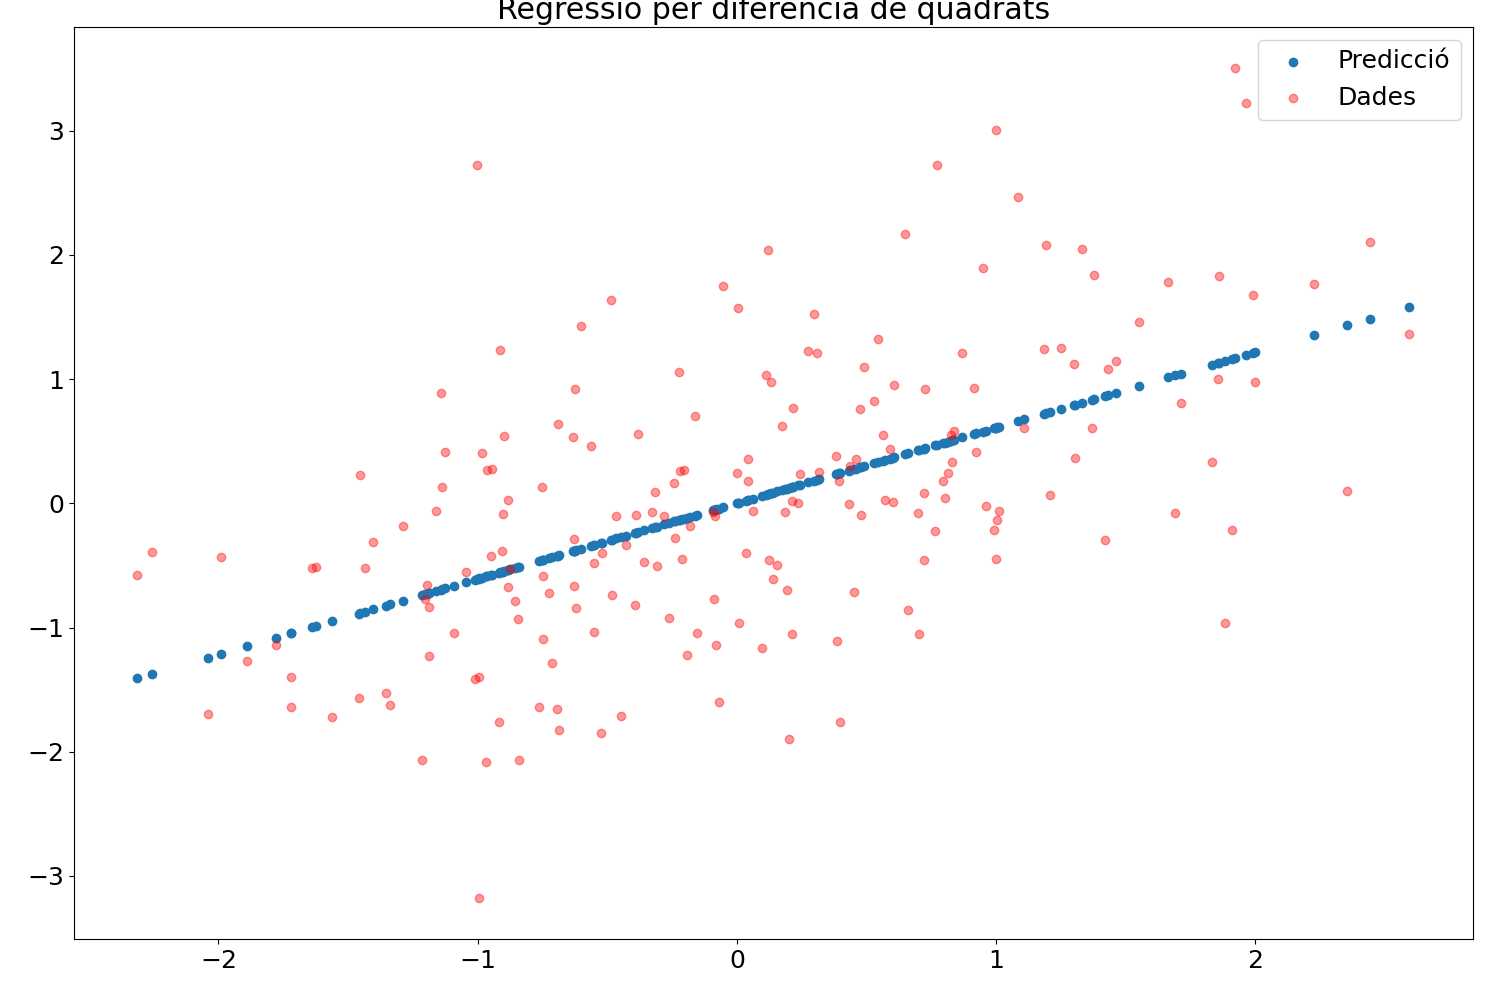
\includegraphics[width=0.7\linewidth]{Figures/least_squares}
	\caption{Exemple d'una regressió lineal de dades generades a l'atzar. Veure el codi a \ref{lst:linear_regression}.}
	\label{fig:leastsquares}
\end{figure}

Hi ha diversos mètodes per ajustar els paràmetres, el més comú és ajustar-los segons la derivada d'una funció anomenada funció de pèrdua o \textit{loss function}, usualment representada per la lletra $\mathcal{L}$. Aquesta funció representa els objectius del programa i pot ser minimitzada o maximitzada, per exemple, en una regressió lienal es vol reduir la distància entre els punts de dades i la línia que prediu la tendència, com es pot veure en la figura \ref{fig:leastsquares}.

Perquè es poden realitzar molts tipus de funcions de pèrdua, ja sigui per la forma de la funció en si o pels paràmetres de la funció, el programes de \textit{machine learning} són extremadament versàtils, la màxima expressió d'això es pot veure en les xarxes neuronals o \textit{neural networks}. Aquests algoritmes són els més potents, complexos i polivalents, dintre de l'aprenentatge automàtic. Precisament utilitzo un d'aquests algoritmes d'aquests per generar les imatges. Reconeixement d'imatges, la traducció i sintetització de textos, la conducció automàtica, els algoritmes de recomanació, i és clar, la generació d'imatges.

\section{Xarxes neuronals}
Aquests tipus d'algoritmes no tenen un nombre que fa recordar a les xarxes de neuronals dels nostres cervells per casualitat, estan directament inspirades en els nostres cervells. Són uns programes que consisteixen en la connexió de diverses operacions anomenades neurones, que conjuntament formen una xarxa, la qual s'organitza a partir de capes. Segons la variació del tipus de neurona i l'estructura que aquestes formen podem tindre algoritmes destinats a fer diferents tasques. Això juntament amb els diversos tipus de funció de pèrdua contribueix a la versatilitat de les xarxes neuronals. Aquests models d'intel·ligència artificial constitueixen el camp del \textit{deep learning} o aprenentatge profund. S'anomenen d'aquesta forma per referenciar la gran profunditat d'aquests algoritmes, és a dir el gran nombre de capes que tenen.

Una neurona consisteix simplement en una suma ponderada, a la qual se li suma un altre número, i finalment una funció no-lineal que s'aplica al resultat. Les neurones tenen vectors com input i output. Per tant, una neurona es pot definir com:
$$
\sigma \left(\sum_{i=1}^n w_i x_i + b\right) = \sigma \left( w_1x_1 + w_2x_2 + \cdots + w_nx_n + b 
\right) 
$$
Per $\sigma$ sent una funció no-lienal i $n$ sent la mida del vector. Després estan els paràmetres, $w_i$ i $b$, anomenats \textit{weights} i \textit{bias}.

Una neurona pot tindre diversos inputs que venen de diverses neurones, el mateix passa amb els outputs. Depenent de com es connectin entre si les neurones, aquestes passen a formar diversos tipus de capes. A partir dels tipus de capes i el nombre d'aquestes és com s'especifica l'arquitectura d'una xarxa neuronal.

Una vegada especificada la interconnectivitat de les neurones puc parlar de la intuïció darrere dels paràmetres, \textit{weight} especifica com és de forta la relació entre una neurona en una capa i una altra neurona en una capa veïna. I un \textit{bias} especifica com és d'important una neurona, ja que aquest número afecta el resultat a la suma, fent que l'activació de la neurona\footnote{Així és com s'anomena el seu resultat.} sigui més alta.

Tornant a l'arquitectura, usualment aquesta es divideix en tres parts la capa d'input, les capes ocultes i la capa d'output. La quantitat de neurones que hi ha a la capa d'inputs és la que defineix la mida del vector que es dona com input a la xarxa, ja que cada element del vector es dona a cada neurona amb la capa. El mateix passa amb la capa d'outputs, cada output de cada neurona de la capa acaba sent un element en el vector que surt de la xarxa. Per tant, el nombre de neurones que té cadascuna d'aquestes dues capes, especifica la mida dels vectors d'input i d'output de la xarxa respectivament. Per exemple, si es vol donar com input a una xarxa una imatge de 16 per 16 píxels\footnote{Una imatge en blanc i negre.} calen 256 neurones en la capa d'inputs, una per cada píxel.

En canvi, les \textit{hidden layers}, és a dir les capes ocultes, no tenen una mida determinada, el mateix passa amb el nombre d'aquestes que té la xarxa. Depenen de cada cas la quantitat de neurones que tenen aquestes capes i també el nombre d'aquestes, varia. Això, juntament amb els diversos tipus de capes és el que dona la versatilitat d'aquests algoritmes.

Entre els diferents tipus de capes que ponen tindre les xarxes neuronals, la més comuna i simple d'aquestes és la \textit{fully connected layer}, o una capa completament connectada, veure la figura \ref{fig:560px-artificialneuralnetwork}. Les neurones que formen aquesta capa estan connectades a totes les neurones de la capa anterior i així mateix, a totes les neurones de la capa següent. Aquestes capes l'única forma de variar que tenen és a partir de canviar el nombre de neurones, ja que no hi ha forma d'alterar el funcionament de les neurones.
\begin{figure}[H]
	\centering
	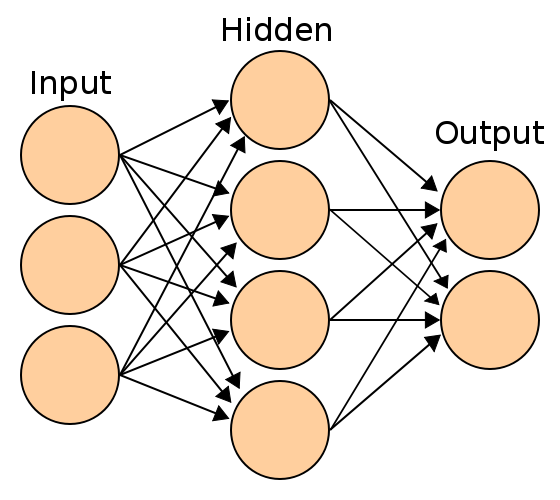
\includegraphics[width=0.7\linewidth]{Figures/560px-Artificial_neural_network.svg}
	\caption{Usualment, les xarxes neuronals es representen d'aquesta forma, amb fletxes i boles. Les boles representarien cada neurona i les fletxes mostren com estan connectades. La \textit{hidden layer} d'aquesta representació es pot veure que és una \textit{fully connected layer} a causa de com està connectada a les altres capes, rebent cada neurona l'output de cada neurona anterior.}
	\label{fig:560px-artificialneuralnetwork}
	% en:User:Cburnett, CC BY-SA 3.0 \href{http://creativecommons.org/licenses/by-sa/3.0/}, via Wikimedia Commons
\end{figure}
No obstant això, es pot variar la funció d'activació que tenen, que ha de ser una funció no lineal. La més utilitzada és la sigmoide:
$$
f(x) = \frac{1}{1+e^{-1}}
$$

\section{Descens del gradient}
Una vegada he parlat de les xarxes neuronals, he de comentar com aquestes evolucionen al llarg del temps, és a dir com se'n van actualitzen a si mateixes per complir el seu objectiu. Ja he comentat que existeix una funció anomenada \textit{loss function}, la qual es deriva per actualitzar els paràmetres de la xarxa. El mecanisme pel qual s'actualitzen els paràmetres s'anomena el descens del gradient.

Aquest procés comença amb la funció de pèrdua, que esmenta els objectius de la xarxa. Els punts mínims d'aquesta funció representen els punts òptims de la xarxa, als quals es vol arribar. 

 Per explicar-lo utilitzaré un exemple pràctic, primer de tot parlaré sobre la funció de pèrdua que s'utilitza i a continuació de l'actualització dels paràmetres. 
 
Parlaré de la classificació d'imatges, si es volen classificar imatges de gats i gossos, s'assignen dues etiquetes a aquestes, per exemple, $1$ als gats i $0$ als gossos. A continuació s'escull una funció de pèrdua\footnote{Una que funcioni per la classificació d'imatges, és clar.} com \textit{binary cross entropy} o \textit{log loss}. La funció \textit{binary cross entropy} és la següent:
\begin{equation}
	\mathcal{L} = - t\log(y) - (1 - t)\log(1 - y) 
	\label{eq:BCE}
\end{equation}
Amb $t_i$ sent l'etiqueta que ha de tenir la imatge, anomenada etiqueta real, i $y_i$ sent l'etiqueta que el model assigna a la imatge. Per tant, si l'etiqueta real és $1$, l'equació acaba sent:
$$
\mathcal{L}_1 = - \log(y)
$$
I el cas contrari per $t = 0$ seria:
$$
\mathcal{L}_0 = - \log(1 - y)
$$

Si donen com input la imatge d'un gat i el programa es dona com output $0.92$ tenim que la pèrdua és de:
\begin{align*}
	\mathcal{L} &= - t\log(y) - (1 - t)\log(1 - y) = - \log(0.92) \simeq 0.0834
\end{align*}
En canvi, si el programa es dona un output de $0.15$ la pèrdua, seria:
\begin{align*}
	\mathcal{L} &= - t\log(y) - (1 - t)\log(1 - y) = - \log(0.15) \simeq 1.897
\end{align*}
Es pot veure que si l'etiqueta que posa el model s'allunya més de l'etiqueta real la pèrdua acaba sent més gran. El mateix es pot veure per les imatges dels gossos, és a dir, les imatges que haurien de tenir etiqueta zero:
\begin{align*}
	\mathcal{L} &= - 0\cdot\log(0.89) - (1 - 0)\cdot\log(1 - 0.89) = - \log(1- 0.89) \simeq 2.207 \\
	\mathcal{L} &= - 0\cdot\log(0.08) - (1 - 0)\cdot\log(1 - 0.08) = - \log(1- 0.08)\simeq 0.0834
\end{align*}
Per tant, com més pròximes estén les prediccions (els outputs del model) a les etiquetes ideals, menor serà la pèrdua. Llavors al minimitzar la funció es trobarà el punt òptim on totes les prediccions seran iguals a les etiquetes.

A aquests punts òptims s'arriben actualitzant els paràmetres a partir de la derivada de la funció, concretament a través del seu gradient. El gradient d'una funció és un vector on els seus elements són la derivada parcial respecte a cada paràmetre (per aclarir, una entrada per paràmetre). El gradient d'una funció $f(\theta)$ es representa com $\nabla f(\theta)$, i es pot escriure en forma de vector com:
$$
\nabla f(\theta) = \begin{bmatrix}
	\pdv{f}{\theta_1} \\
	\pdv{f}{\theta_2} \\
	\vdots \\
	\pdv{f}{\theta_{n-1}} \\
	\pdv{f}{\theta_{n}}
\end{bmatrix}
$$
No fa falta fixar-se en el que és exactament un gradient, només s'ha de saber que cada paràmetre de la xarxa neuronal\footnote{Cada \textit{weight} i cada \textit{bias}.} s'ha d'actualitzar d'acord amb la derivada respecte al paràmetre. Això es pot entendre com canviar lleugerament un paràmetre d'acord amb la direcció de la derivada respecte a ell. L'objecte que s'encarrega d'actualitzar-los s'anomena optimitzador. L'optimitzador més senzill que hi ha és el següent:
\begin{equation}
	\theta_{i}^t = \theta_{i}^{t-1} \pm \eta\pdv{\mathcal{L}(\theta)}{\theta_{i}^{t-1}}
	\label{eq:optimizator}
\end{equation}
Es pot veure com s'actualitza el paràmetre $\theta_i$. En l'equació he posat el superíndex $t$ per expressar aquesta actualització, passant d'un temps $t-1$ a $t$. A més a més, utilitzo el símbol $\theta$ per expressar tots els paràmetres del model. En els optimitzadors s'afegeix un nombre $\eta$ anomenat \textit{learning rate}. Usualment, és un nombre petit\footnote{Entre $0.1$ i $0.001$ per exemple.}, aquest nombre especifica com de ràpid canvien els paràmetres. El \textit{learning rate} es pot anar ajustant depenen de la situació o del model en el qual s'implementi. Alteracions en aquest poden causar diversos fenòmens tant negatius com positius.

Cal notar que en l'optimitzador he utilitzat el signe $\pm$ perquè si és positiu significa que s'està ascendint pel gradient, i si és negatiu s'està descendint. No obstant això, usualment es fa servir el signe negatiu per convenció, ja que la majoria de funcions de pèrdua estan dissenyades per ser descendides.

Al fer la derivada de la funció de pèrdua es pot veure immediatament que s'ha d'aplicar la regla de la cadena, ja que l'estructura de la xarxa neuronal està composta per una sèrie de funcions compostes entre si. En la secció següent parlaré del procediment que s'utilitza per avaluar el gradient, anomenat \textit{backpropagation} o propagació inversa.

\subsection{Backpropagation}
Al aplicar la regla de la cadena «de fora cap a dins» s'ha de començar a derivar per l'última capa i acabar per la primera, d'aquí ve el nom \textit{backpropagation} perquè es propaga l'error en direcció contrària. Mentre que quan es dona un input a la xarxa, s'anomena {forward propagation} o \textit{forward pass}.

No entraré en profunditat sobre l'intuïció de la \textit{backpropagation} en aquesta secció, només em limitaré a esmentar la manera en la qual es calcula.

L'activació\footnote{S'anomena així al resultat d'una neurona.} d'una neurona $j$ en l'última capa $L$ de la xarxa es defineix com: 
$$
a^{L}_j = \sigma\left(\sum_{j=0}^{n_{L- 1}}w^L_{jk} a^{L-1}_k+ b_j^L\right)
$$
On $a^{L-1}_k$ és l'activació d'una neurona $k$ en la capa anterior $L-1$, i on el \textit{weight} $w^L_{jk}$ és el paràmetre que expressa en què mesura es connecta la neurona $j$ a la neurona $k$. Com ja he dit, expressa com és de forta aquesta connexió. La suma es fa al llarg de $n_{L-1}$ que és el nombre de neurones que té la capa $L-1$. Utilitzant aquesta definició ja es poden efectuar les derivades.

No obstant això, convé definir el terme $z_j^L$ per procedir a fer les derivades. Simplement, és l'equació d'una neurona però sense la funció d'activació:
\begin{equation}
\label{eq:neuron_definition}
	z_j^L = \sum_{j=0}^{n_L - 1}w^L_{jk} a^{L-1}_k+ b_j^L
\end{equation}
L'objectiu és obtenir la derivada de la \textit{loss function} respecte a un \textit{weight} qualsevol i un \textit{bias} qualsevol. Per tant, s'han de obtenir les següents derivades parcials:
$$
\pdv{\mathcal{L}}{w_{jk}^L} \text{ i } \pdv{\mathcal{L}}{b_j^L}
$$
Començaré amb la derivada del \textit{weight}, al aplicar la regla de cadena obtenim que:
\begin{equation}
	\pdv{\mathcal{L}}{w_{jk}^L} = \pdv{z_k^L}{w_{jk}^L}\pdv{a_j^L}{z_j^L}\pdv{\mathcal{L}}{a_j^L}
	\label{eq:chain_neuron}
\end{equation}
La primera derivada, és la derivada de $z_j^L$ respecte al \textit{weight}:
\begin{equation*}
	\pdv{z_j^L}{w_{jk}^L} = a^{L-1}_k
\end{equation*}

La següent és la derivada del resultat de la neurona $a_j^L$ respecte a $z_j^L$, que resulta ser la derivada de la funció d'activació de la neurona:
\begin{equation*}
	\pdv{a_j^L}{z_j^L} = \sigma'(z_j^L)
\end{equation*}

Finalment, està la derivada de la funció de pèrdua respecte a l'output de la xarxa, és a dir, l'activació d'una de les últimes neurones. La qual és simplement la derivada de la funció de pèrdua, per tant, varia en cada cas.

Ja sabent totes les derivades, es pot reescriure l'equació \ref{eq:chain_neuron} es pot escriure com\footnote{Deixo l'última derivada $\pdv{\mathcal{L}}{a_j^L}$ sense reescriure perquè aquest terme pot variar depenent de la funció de pèrdua que s'utilitza.}:
$$
	\pdv{\mathcal{L}}{w_{jk}^L} = \pdv{z_k^L}{w_{jk}^L}\pdv{a_j^L}{z_j^L}\pdv{\mathcal{L}}{a_j^L} = 
	a^{L-1}_k \sigma'(z_j^L)\pdv{\mathcal{L}}{a_j^L}
$$

No obstant falta un detall, per efectuar la derivada de l'activació d'una neurona respecte a la funció de pèrdua s'ha d'afegir un sumatori:
$$
\pdv{\mathcal{L}}{a_j^{L-1}} = \sum_{j=0}^{n_{L-1}} \pdv{z_j^L}{a_k^{L-1}}\pdv{a_j^L}{z_j^L}\pdv{\mathcal{L}}{a_j^L}
$$
La suma representa que aquesta neurona té un output que es propaga cap endavant afectant les neurones que la segueixen.

Finalment, he d'esmentar la derivada de la funció de pèrdua respecte a un \textit{bias} qualsevol $ b^L_k$. Al aplicar la regla de la cadena es pot veure que aquesta derivada és:
\begin{equation*}
	\pdv{\mathcal{L}}{b^L_k} = \pdv{z^L_{k}}{b^L_{k}}\pdv{a^L_{k}}{z^L_{k}}\pdv{\mathcal{L}}{a^L_{k}}
\end{equation*}

Al veure l'equació \ref{eq:neuron_definition} es pot veure que la derivada $ \pdv{z^{L}_{k}}{b^{L}_{k}}$ serà $1$ pel fet que $ b^{L}_{k}$ és una constant. Les altres derivades de l'equació ja les he esmentat anteriorment. Per tant, finalment tenim que:
\begin{align*}
	\pdv{\mathcal{L}}{w_{jk}^L} &= a^{L-1}_k \sigma'(z_j^L)\pdv{\mathcal{L}}{a_j^L} \\
	\pdv{\mathcal{L}}{b^L_k} &= \sigma'(z_j^L)\pdv{\mathcal{L}}{a_j^L}
\end{align*}

Amb aquestes derivades ja es pot desenvolupar el vector gradient, que com ja he dit està compost per les derivades de cada paràmetre de la xarxa, no obstant això, concretament està compost la mitjana d'aquestes, perquè es vol actualitzar els paràmetres per poder minimitzar la pèrdua en totes les dades disponibles. Per tant, es calcula l'error d'unes quantes mostres del \textit{dataset}, i s'efectua una mitjana d'aquests errors.

Tota aquesta teoria es veurà implementada en la part pràctica en forma de codi, ja que m'he vist amb la necessitat de tenir una xarxa neuronal programada des de zero. No obstant això, usualment s'utilitzen plataformes com \textit{TensorFlow} \cite{tensorflow2015-whitepaper} o \textit{PyTorch} \cite{pytorch_2019} al programar xarxes neuronals, pel fet que aquests \textit{frameworks} faciliten moltíssim el treball als programadors.

\section{Generative adversial networks}
Com ja he dit hi ha molts tipus de xarxes neuronals, tanmateix, en aquest treball només em centraré en un tipus en específic, les xarxes generatives adversatives o \textit{generative adversial networks (GAN)} en anglès.

Aquestes xarxes, com el seu nom diu, s'utilitzen per generar dades, usualment s'apliquen a imatges. Es troben al darrere de projectes com \textit{This person does not exist} \cite{styleGAN, this_person_does_not_exist}, una pàgina web que et genera una cara d'una persona que no existeix, ja que és una cara generada artificialment a partir d'aquest tipus de models.

Aquests tipus de models van ser introduïts per primera vegada en 2014 per Ian Goodfellow \cite{GAN2014}, des de llavors s'han convertit en un dels models de \textit{deep learning} més sòlids i utilitzats.

Aquests algoritmes consisteixen en dos models (xarxes) diferents, un generador i un discriminador, amb objectius oposats. Per aquesta raó s'inclou paraula adversativa en el nom. El generador i discriminador es poden entendre com un falsificador de bitllets i uns policies que el vol atrapar. On el generador és el falsificador de bitllets i el discriminador és el policia.

L'analogia és la següent: 
Una vegada el falsificador comença el seu entramat, el policia contesta immediatament, i amb el temps es torna millor al seu treball, podent distingir entre els bitllets falsificats i els reals. El falsificador respon a això millorant les seves tècniques, per tant, el policia han de millorar encara més. És un cicle en el qual aquestes forces antagonistes es fan millorar l'una a l'altra.

El mateix passa amb el generador i el discriminador. El discriminador aprèn a distingir entre les imatges reals i les imatges falses que fabrica el generador, mentre que el generador aprèn a enganyar al discriminador. 

Si s'especifiquen bé els objectius de cada model, arriben a \textit{zero sum game}\footnote{Un \textit{zero sum game}, és simplement un joc entre dos jugadors que per guanyar un, l'altre ha de perdre e.g. joc d'estirar la corda entre dos equips.}. La manera en la qual es soluciona aquest tipus de joc és arribant a un equilibri de Nash \cite{QGAN_exp}, on el discriminador no sap diferenciar entre les imatges reals i les falses\footnote{Que el discriminador no sàpiga diferenciar no implica arribar a un equilibri de Nash, aquest concepte és definit d'una altra forma que està fora de l'àmbit d'aquest treball \cite{GAN2014}.}.

En l'article original \cite{GAN2014}, s'esmenta un pseudocodi per aquests models, que he representat en l'algoritme \ref{alg:GAN}. En aquest es parla de \textit{minibatch} que és simplement un grup d'imatges o de dades, i de soroll, que són dades generades aleatòriament i que es donen com input al generador perquè aquest no generi exactament les mateixes imatges cada vegada. El soroll afegeix variació als outputs del generador, però sempre s'intenta que sigui en una petita quantitat.

\begin{algorithm}[H]
	\caption{Pseudocodi per una xarxa generativa adversativa}\label{alg:GAN}
	\begin{algorithmic}
		\For{número de interaccions}
		\For{$k$ pasos}
		\State Treure minibatch de $m$ mostres de soroll $\{z_i, \cdots, z_m\}$ de la distribució de soroll $p_g(z)$
		\State Treure minibatch de $m$ mostres d'exemples $\{x_i, \cdots, x_m\}$ de la distribució d'exemples $p_{\mathrm{data}}(x)$
		\State Actualitzar el discriminador ascendint el seu gradient: 
		$$
		\nabla_\theta \frac{1}{m}\sum_{i=1}^{m}\left[\log D(x_i) + \log(1- D(G(z_i)))\right]
		$$
		\EndFor
		\State Treure minibatch de $m$ mostres de soroll $\{z_i, \cdots, z_m\}$ de la distribució de soroll $p_g(z)$
		\State Actualitzar el generador descendent el seu gradient:
		$$
		\nabla_\theta \frac{1}{m} \sum_{i=1}^{m} \log(1-D(G(z_i)))
		$$
		\EndFor
	\end{algorithmic}

\end{algorithm}

En el pseudocodi es pot veure que primer s'actualitza el discriminador $k$ vegades i després  el generador una sola vegada. Això és perquè interessa que el discriminador sàpiga distingir les imatges ràpidament, per poder indicar al generador com generar les imatges. Si el discriminador esmenta que unes imatges de gats són imatges de gossos, el generador fabricarà imatges de gossos pensant que ho són de gats, perquè aquest aprèn a partir del que l'indica el discriminador.

També és pot veure com és la funció de pèrdua, que en l'article els autors anomenen \textit{Minimax loss function}, la qual en la pràctica és la mateixa que la \textit{Binary Cross Entropy (BCE)}. Es pot veure que en la BCE, quan $t=0$, que seria l'etiqueta per les imatges falses del generador, aquesta funció seria $\log(1-y)$. En el cas contrari, per $t=1$, la funció seria $\log(y)$.



\chapter{Generació d'imatges amb un ordinador quàntic}

Investigadors en informació quàntica al veure el potencial que tenen els ordinadors quàntics i la intel·ligència artificial, no es van poder resistir a crear un nou camp d'investigació, el \textit{Quantum Machine Learning (QML)}, o aprenentatge automàtic quàntic. Igual que les xarxes neuronals són les estrelles dintre del \textit{machine learning}, les xarxes neuronals quàntiques també ho són dintre del \textit{quantum machine learning}.

Des de que es van començar a investigar aquests algoritmes s'han arribat a implementar diversos tipus de xarxes neuronals. Principalment pel que fa a la generació i classificació d'imatges i dades.

No obstant això, aquests algoritmes no són completament quàntics, usualment consisteixen a actualitzar els paràmetres d'un circuit quàntic perquè aquest generi les dades. On les actualitzacions dels paràmetres es calculen amb un ordinador clàssic. Això es veurà molt clar quan expliqui la part pràctica del treball.

Abans de continuar amb la secció he de dir que existeixen diversos algoritmes dintre del \textit{quantum machine learning}, no tot en la vida són xarxes neuronals. Per exemple, es pot donar a terme classificació de dades mitjançant \textit{support vector machines}\footnote{Classificar dades de dimensions petites en espais vectorials molt grans.} \cite{QSVM_2019, QSVM_xanadu_2019} o amb un anàleg de la regressió lineal \cite{Q_linear_regression_xanadu}. Malgrat això, en aquest capítol em centraré exclusivament en les xarxes neuronals quàntiques.

\section{Descens del gradient quàntic}
De moment tindre en consideració que una xarxa neuronal quàntica és un circuit quàntic qualsevol, però parametritzat, és a dir, que té portes quàntiques parametritzades. Això juntament amb una funció de pèrdua i un \textit{dataset} és suficient per explicar com s'actualitzen els paràmetres.

L'objectiu principal és avaluar la derivada respecte a un paràmetre. Sorprenentment, és dona a terme d'una manera més senzilla que amb una xarxa neuronal clàssica. Tan sols s'utilitza la definició de la derivada per poder avaluar-la: S'altera lleugerament un sol paràmetre i es treu la diferència entre dos outputs del circuit quàntic que tenen el paràmetre alterat. Aquest mètode per avaluar la derivada s'anomena \textit{parameter shift} \cite{tfq, shift_parameter_harrow_2019}.

Si un circuit quàntic té un vector de paràmetres $\theta\,$, per un paràmetre $\theta_{i}\,$, es defineix un vector de pertubació $\Delta_i$ ple de zeros, d'igual mida que $\theta$, però que en la posició de $\theta_i$ té un $1$. A partir del vector de pertubació es pot definir la derivada de la funció de pèrdua $\mathcal{L}(\cdot)$ respecte al paràmetre $\theta_{i}\,$:
$$
\pdv{\theta_i} \mathcal{L}(\theta) = \mathcal{L}(\theta + \tfrac{\pi}{4}\Delta_i) - \mathcal{L}(\theta - \tfrac{\pi}{4}\Delta_i)
$$
Es pot veure que el vector $\theta \pm \frac{\pi}{4}\Delta_i$ és el vector $\theta$, però amb una petita variació en la posició $i$ que és la que correspon al paràmetre $\theta_i\,$. Amb aquest mètode ja es pot desenvolupar pràcticament qualsevol actualització de paràmetres, aquesta és la part senzilla de les xarxes neuronals quàntiques, la dificultat radica en la forma dels circuits quàntics que les componen.

\section{Circuits quàntics per xarxes neuronals}
\label{qcircuits}
L'única qualitat obligatòria que hi han de dintre aquests circuits és que han d'estar parametritzats. Usualment, estan compostos per una gran quantitat de portes rotacionals parametritzades, les quals ja he presentat en les equacions \ref{eq:rx}, \ref{eq:ry} i \ref{eq:rz}.

El problema al qual s'enfronten els investigadors dedicats a les xarxes neuronals quàntiques és la manera amb la qual implementar funcions no-lienals en els circuits quàntics. Aquests tipus de funcions són les responsables de la gran complexitat i profunditat de les xarxes neuronals clàssiques. A primera vista pot semblar una tasca quasi impossible a causa de la naturalesa lineal de la computació quàntica. Tanmateix, durant els anys s'han desenvolupat diverses tècniques per donar a terme aquesta fita, les quals comentaré a continuació.

A partir d'una combinació de rotacions i portes que entrellacen qubits es pot arribar a implementar una funció semblant a la tangent hiperbòlica\footnote{La tangent hiperbòlica també s'utilitza com a funció no-lienal en el \textit{deep learning}.} en un circuit quàntic \cite{cao2017quantum}. No obstant això, aquest mètode té un gran desavantatge, consisteix en un circuit que s'ha d'anar mesurant i repetint per veure si funciona correctament, els autors parlen de \textit{repeat until success} perquè s'ha de mesurar un qubit i mirar si dona $\ket{0}$ per assegurar que aquesta funció ha sigut aplicada correctament\footnote{En cas que doni $\ket{1}$, s'ha de repetir el procés.}.

En un article posterior\footnote{Realitzat en part per un dels autors del mètode anterior.}, en el qual els autors generen distribucions contínues a partir d'una xarxa generativa adversària quàntica.
S'especifica que les no-linearitats presents en l'algoritme no formen part del circuit quàntic, és a dir, funcions que s'implementen clàssicament als resultats dels circuits quàntics o a les dades que s'introdueixen als circuits \cite{romero2019variational}. Aquesta és una mesura molt simple que possiblement implementaré durant la part experimental.

En 2019 es va publicar un dels articles que més m'agraden\footnote{Utilitzen imatges de gats a les figures i és un dels primers articles que vaig llegir d'aquest camp fa més de dos anys. A més a més la xarxa neuronal esmentada en l'article està completament programada en TensorFlow Quantum \cite{tfq}, i això sempre s'agraeix. } Cong et. al. (2019) \cite{cong2019convolucional}, en ell els autors presenten una xarxa neuronal convolucional quàntica. No fa falta entrar en detall, però es diuen convolucionals perquè s'apliquen convolucions a les imatges que es volen classificar, es multiplica una part de la imatge per una matriu que s'anomena filtre \cite{CNN}. Simplement, tenen un altre tipus de capes que no són les capes completament connectades. L'única afirmació dels autors que s'ha de recalcar, és que a partir de reduir els graus de llibertat (\textit{degrees of freedom}) en els circuits quàntics, sorgeixen no-linearitats. Això és a causa dels mesuraments parcials que es donen a terme en un moment determinat de l'algoritme.

Un dels mètodes que m'ha semblat més interessant, és l'implementat en una altra xarxa convolucional quàntica, on a l'aplicar els filtres que s'utilitzen per a la convolució, s'implementa una funció no-lienal. Aquest mètode no el puc arribar a comprendre, les equacions que fan servir són molt complexes i no sembla que arriben a utilitzar un mesurament parcial en cap moment. Simplement, els autors presenten una equació i diuen que no és lienal, i no puc arribar a comprendre perquè ho és.

Finalment, he de parlar de l'article que he seguit per fer aquest treball, Huang et. al. (2021) \cite{QGAN_exp}, en aquest, al igual que en l'article de Cong et. el. (2019) \cite{cong2019convolucional}, s'utilitzen mesuraments quàntics per introduir no-linearitats a l'algoritme. Concretament, els autors implementen aquests mesuraments tant en el generador quàntic d'imatges, com en el discriminador. Els circuits quàntics que utilitzen per al generador d'imatges tenen la següent forma:

\begin{center}
	\begin{quantikz}
		\lstick[wires=2]{$\mathcal{A}$}& & \lstick{$\ket{0}$} &  \gate{R_y(\alpha_1)}\gategroup[5,steps=1 ,style={dashed,
			rounded corners,fill=green!20, inner xsep=2pt},background]{$\ket{z}$ estat inicial} & \gate{U_{\theta_{1, l}}}\gategroup[5,steps=5 ,style={dashed,
		rounded corners,fill=blue!20, inner xsep=2pt},background]{repetició $l$} & \ctrl{1} & \qw & \qw & \qw & \gate{U_{\theta_{1, l-1}}} & \ctrl{1} & \qw & \qw & \qw & \qw \\
		& & \lstick{$\ket{0}$} &  \gate{R_y(\alpha_2)} & \gate{U_{\theta_{2, l}}} & \control{} & \ctrl{1} & \qw & \qw & \gate{U_{\theta_{2, l-1}}} & \control{} & \ctrl{1} & \qw & \qw & \qw \\
		&&\lstick{$\ket{0}$} &  \gate{R_y(\alpha_3)} & \gate{U_{\theta_{3, l}}} & \qw & \control{} & \ctrl{1} & \qw & \gate{U_{\theta_{3, l-1}}} & \qw & \control{} & \ctrl{1} & \qw & \qw \\
		&&\lstick{$\ket{0}$} &  \gate{R_y(\alpha_4)} & \gate{U_{\theta_{4, l}}} & \qw & \qw & \control{} & \ctrl{1} & \gate{U_{\theta_{4, l-1}}} & \qw & \qw & \control{} & \ctrl{1} & \qw \\
		&&\lstick{$\ket{0}$} &  \gate{R_y(\alpha_5)} & \gate{U_{\theta_{5, l}}} & \qw & \qw & \qw & \control{} & \gate{U_{\theta_{5, l-1}}} & \qw & \qw & \qw & \control{} & \qw
	\end{quantikz}
\end{center}

On les portes $R_y$ amb un paràmetre $\alpha_i$, marcades en verd, són utilitzades per introduir les dades al circuit. Aquestes dades són simplement soroll que crea varietat en els outputs dels circuits, igual que el soroll que s'empra en les GAN clàssiques (algoritme \ref{alg:GAN}).

El circuit que genera les imatges realment consisteix en les portes $U_{\theta}$ i $\mathrm{CZ}$, marcades en blau. Aquestes portes s'agrupen en les repeticions-$l$, que s'utilitzen per afegir profunditat i complexitat als circuits. En aquest cas el circuit té dues repeticions-$l$\footnote{És a dir $l=2$.}. Al mesurar es fa un mesurament parcial, però els autors especifiquen que es fa d'una forma concreta que explicaré a continuació.

Per un estat $\ket{\Psi_\alpha}$ que surt del circuit especificat posteriorment, l'estat $\rho(z)$ després d'una mesura parcial sobre el qubits $\mathcal{A}$, és:
$$
\rho(z) = \frac{\tr_\mathcal{A}(\Pi_\mathcal{A}\ket{\Psi(z)}\bra{\Psi(z)})}{\tr(\Pi_\mathcal{A} \otimes I_{2^{N-N_\mathcal{A}}}\ket{\Psi(z)}\bra{\Psi(z)})}
$$
Els autors afirmen que aquest estat $\rho(\alpha)$, és una funció no-lineal de l'estat $\ket{z}$. Això és degut al fet que tant el denominador com el numerador de l'equació són funcions de $\ket{z}$.

Tanmateix, en altres treballs com per exemple Zoufal et.al. (2019) \cite{QGAN_IBM}, on es defineix una GAN quàntica que genera distribucions de probabilitat, els autors no mencionen la necessitat de tenir funcions no lineals en alguna part de l'algoritme.



	
	\chapter{Experimental Work}
	\label{chap:experimental_work}
	\chapter{Plantejament de l'hipòtesi}

Al ser l'implementació de les funcions no-lineal un assumpte lleugerament conflictiu entre els diversos models de xarxes neuronals quàntiques havia decidit des de un principi centrar-me en aquest assumpte en concret. Podria haver anat per al altres vies com la generació d'imatges amb color o l'implementació d'un d'una porta $X$ en una part especifica del circuit quàntic que genera les imatges, que al posar-la o no, el model generes dos tipus d'imatge a través del mateix circuit. Tanmateix, les dues propostes requerien de desenvolupar nous conceptes, llavors al no tindre el coneixements necessaris per poder desenvolupar-les vaig descartar aquestes opcions. 

La pregunta a investigar és la següent: \\
L'incorporació d'una funció no-lineal en el circuit quàntic del model, a partir d'una mesura parcial, causa que el model arribi més ràpidament al punt òptim?

En altres paraules, volia veure si la mesura parcial repercutia positivament en la eficiència del model, fent que la generació de les imatges desitjades es dones a terme en un menor temps. 

Sembla una qüestió senzilla, però la dificultat del experiment radica en crear la xarxa neuronal en si, amb totes les seves parts accessibles per poder fer els canvis que siguin necessaris. L'única manera de fer-ho seria programant el model. 

\chapter{Programació del model}

Posteriorment a començar a programar el model, jo ja sabia que ho havia de realitzar en Python, ja creat petits algoritmes abans de començar aquest treball i tenia experiència construint i executant circuits quàntics amb Cirq, una eina desenvolupada per Google. A més a més, sabia de l'existència de TensorFlow Quantum \cite{tfq}, una altra eina desenvolupada per Google destinada a la creació de xarxes neuronals quàntiques i algoritmes de \textit{quantum mechine learning} en general. També tenia experiència en aquest \textit{framework}. Llavors TensorFlow Quantum va ser la meva primera opció, tenia pensat basar el meu codi en el tutorial de TensorFlow sobre un xarxa convolucional generativa adverbial. Havia de canviar el generador per un circuit quàntic que s'obtimitza a partir d'un diferenciador automàtic provinent de TensorFlow Quantum. Els canvis que corresponien al discriminador simplement havien de ser un canvi d'arquitectura, passar d'una xarxa més complexa a una de més simple que només consistia en unes poques capes totalment connectades. 

El primer problema que em vaig trobar va ser la creació del \textit{data set} que alimentar a la xarxa discriminativa. A causa de la peculiaritat de les imatges que volia generar\footnote{Usualment les imatges que componen els \textit{datasets} utilitzats en \textit{deep machine learning} són extretes de bancs d'informació amb mides enormes. En el meu cas, havien de ser generades per mi, per tant havia de convertir matrius de Numpy en \textit{datasets} per TensorFlow.}. Recordo que en va costar arribar a tindre la solució a aquest problema. 

\section{Discriminador}

Una vegada ja tenia fet el \textit{dataset} em vaig posar a fer el model. En el tutorial per una \href{https://www.tensorflow.org/tutorials/generative/dcgan}{DCGAN (GAN conolucional)} els dos models eren entrenats per la funció \code{train\_step}. En aquesta es crida a la funció \code{tf.GradientTape} per guardar el diferenciador automàtic. El problema que vaig dintre amb aquesta funció es que directament no funcionava amb el discriminador, aquest no era optimitzat. Després de intentar solucionar l'error pels meus propis medis, mirant la causa d'aquest i de buscar a forums la solució o causa, em vaig rendir. Ja havia estat uns quants mesos intentant desenvolupant el model amb TensorFlow i TensorFlow Quantum. Havia creat les capes del generador quàntic manualment, també ho havia fet amb el optimitzador. Tenia el model gairebé acabat, però al no poder optimitzar el discriminador em vaig veure obligat a canviar d'estrateiga. 

Existeixen dos grans \textit{frameworks} per crear i executar circuits quàntics: Cirq \cite{cirq}, desenvolupat per Google i Qiskit \cite{qiskit}, creat per IBM. Una vegada vaig decidir no continuar amb Cirq, havia de provar amb Qiskit. La veritat, havia d'haber començar amb Qiskit des de el principi, és més útil (té moltes més característiques), i el més important, té una gran comunitat, per tant, es més fàcil trobar solucions als error que pots tenir i és més fàcil trobar a persones disposades a ajudar-te.

Al igual que Cirq té un \textit{framework} per poder desenvolupar xarxes neuronals, TensorFlow Quantum, Qiskit també té el seu PyTorch \cite{pytorch_2019}, no obstant no té una integració tan directa, ja que no estan desenvolupats per el mateix equip, ni la mateixa companyia. 

Per tant, al canviar de Cirq a Qiskit, també havia de canviar de TensorFlow a PyTorch, no obstant, no tenia res d'experiencia amb PyTorch, sabia que seria més complicat, i tenia raó. No vaig ni aconseguir crear el \textit{dataset} que contenia les imatges que alimentar al discriminador. 

Després d'intetar-lo amb TensorFlow Quantum i amb PyTorch, vaig decidir prescindir de \textit{frameworks} per crear models de \textit{machine learning}, el discriminador, al ser una xarxa tan simple, la podia crear des de zero. Llavors vaig començar a buscar codi, d'una xarxa neuronal que havia estat feta amb Numpy, una llibreria de Python per fer càlculs amb vectors i matrius que havia fer servir des de que vaig començar amb Python.

Després de provar dues opcions que més o menys m'agradaven\footnote{Busca codi estructurat d'una forma en concret, que estigui dissenyat amb \textit{Object Oriented Programming}, una forma d'escriure codi en el qual tot s'implementa en un objecte.}, va aparèixer un repositori\footnote{\href{https://github.com/mnielsen/neural-networks-and-deep-learning}{link del respositori}} de Michael Nielsen, un dels autors de \textit{Quantum Computation and Quantum Information} \cite{QCandQI} que em va salvar. 

El repositori tenia codi que estava estructurat d'una forma que m'agradaba i encara més important, que l'entenia. Inclús tènia diverses versions d'una xarxa neuronal, amb un nivell de complexitat diferent. Llavors, a partir del model més simple que havia en el repositori, veure el codi original al apèndix \ref{lst:disc_original}, vaig començar a desenvolupar el discriminador. 

Com es pot veure al codi final per el discriminador, he fet bastants canvis, però ho he canviat l'estructura o el funcionament teòric, la majoria són per tindre més funcionalitat, com per exemple l'enmagatzematge de les dades per poder al final veure-les en gràfic. Però el canvi més important és que inclou les dues formes d'optimitzar el model, amb dues funcions de pèrdua que funcionen de manera diferents però que són el mateix, la \textit{Binary Cross Entropy} i la \textit{MinMax}. Ja he parlat d'aquestes dues funcions en la part teòrica del treball, però a mode de recordatori, amb la primera s'agafa una imatge falsa o una real, i s'altera la funció, mentre que amb la \textit{MinMax} depenent de si es una imatge falsa o una real, s'utilitza una funció diferent. Això en el codi està materialitzat en dues funcions\footnote{Funcions de Python.} diferents, \code{backprop\_bce()} i \code{backprop\_minimax()}. No fa falta entrar en detall sobre que va cadascuna de les funcions, degut a que, fan el mateix i no tenen ninguna diferencia en termes de eficàcia o rapidesa. Les vaig fer tan sols per comprovar que no hi hauria ninguna diferencia. El codi final del discriminadors es pot veure al apèndix \ref{lst:disc_final}. També en el repositori del treball hi ha un altre arxiu anomenat \code{discriminator.py}, que conté una altre versió en la qual intentava implementar diverses funcions d'activació en el model, però no ho vaig aconseguir, tanmateix, no em preocupa perquè no es una part vital del treball, no passa res per tindre el discriminador només amb la sigmoide. 

\section{Generador}

El desenvolupament de l'altre part del model, el generador, va ser molt diferent. Després de provar a fer-ho amb TensorFlow, sense resultats, no tenia altra opció que fer-ho tot manualment i jo mateix\footnote{No em vaig ni plantejar buscar codi per internet perquè pensava que els autors dels paper que vaig llegir, les úniques persones que sabia que podien tindre el codi, no el penjarien.}, no obstant, ja tenia experiència en fer pseudo-xarxes neuronals quàntiques. Sabia perfectament el que tenia que fer, i com ho havia de fer. Implementar el mètode de \textit{parameter shift} en els circuits quàntics de l'article en el que vaig basar el treball \cite{QGAN_exp}. 

Una vegada vaig crear els circuits quàntics amb una funció fins a un punt en el qual sentia que ja estava tot perfecte, em vaig posar amb la optimització. 

Penso que és més fàcil de fer que el \textit{backpropagation} en una xarxa neuronal clàssica. 
Primer de tot cal remarcar que el model s'optimitza a partir d'un \textit{batch}, es a dir, un grup d'imatges, en aquest cas, un grup de dades, extretes del \textit{latent space}. Per tant, s'agafa la mitjana del errors de cada input, i s'actualizen els paràmetres a partir d'aquesta mitjana. No es mira l'error d'un sol input per optimitzar, s'ha de mirar el de uns quants, s'aquesta manera, l'optimtizació és més robusta. 

El procediment és el següent, s'ha d'agafar els paràmetres a optimitzar, que estaran en la forma d'un vector, escollir un dels paràmetres, i crear el vector de pertubació. Es a dir un vector de la mateixa mida que el vector amb els paràmetres, però amb tot de zeros, menys a la posició del paràmetres que es vol optimitzar. 

Llavors es creen dos vectors de paràmetres nous multiplicant $\pm\frac{\pi}{4}$ pel vector de pertubació, i sumant el resultat al vector de paràmetres original. A continuació, es creen dues imatges, cadascuna per a cada grup de paràmetres, una amb el terme $\pm\frac{\pi}{4}$ positiu i l'altra amb el negatiu. Per últim, es mira la funció de pèrdua per a cada imatge generada i es treu la diferencia entre elles. El resultat es sumat a un vector que té la mateixa mida que el vector de paràmetres. Al començament de l'iteració, aquest vector és zero, però segons es va optimitzat s'ha li van sumant els errors. Això es fa per a cada paràmetre del circuit per un input, i per a cada input dintre del \textit{batch} a optimitzar.
\begin{figure}
	\label{fig:alg_gen}
	\HRule \\[-.5cm]
	\begin{algorithmic}[1]
		\State{$\nabla = 0$} \Comment{Creació del vector  $\nabla$ que te la mateixa mida que $\theta$}
		\For{soroll en batch}
		\For{paràmetre $\theta_i$ en  $\theta$}
		\State{$\Delta_i = 0$} \Comment{Creació del vector pertubació d'acord amb el vector $\theta_i$}
		\State{$\theta^{+}_i = \theta + \frac{\pi}{4}\Delta_i$}
		\State{$\theta^{-}_i = \theta - \frac{\pi}{4}\Delta_i$}
		\\
		\State{Imatge\textsubscript{1} = generador(soroll, $\theta^+_i$) } 
		\State{Imatge\textsubscript{2} = generador(soroll, $\theta^-_i$) } \Comment{Generació de les imatges}
		\\
		\State{Predicció\textsubscript{1} = discriminador(Imatge\textsubscript{1})} 	\State{Predicció\textsubscript{2} = discriminador(Imatge\textsubscript{2})} \Comment{El discriminador posa una etiqueta a cada imatge}
		\\
		\State{Diferencia\textsubscript{$i$} = $\mathcal{L}$(Predicció\textsubscript{1}) - $\mathcal{L}$(Predicció\textsubscript{2})}
		\\
		\State{$\nabla_\theta = \nabla_i + $ Diferencia\textsubscript{$i$}} \Comment{On $\mathcal{L}$ és la funció de pèrdua del generador}
		\EndFor
		\EndFor
		\\
		\For{$\theta_i$ en $\theta$ i $\nabla_i$ en $\nabla_\theta$} \Comment{Per a cada paràmetre i per a cada error}
		\State{$\theta^{t+1}_i = \theta_i + \frac{\eta}{M}\nabla_i$} \Comment{Actualització del paràmetre amb la mitjana de l'error que correspon a aquest paràmetre}
		\EndFor
	\end{algorithmic}
	\HRule \\[-.4cm]
	\caption{\textbf{Pseudocodi per una xarxa generativa adversativa.} Em refereixo al input de la xarxa generacional com a soroll, ja que és més acertat d'aquesta manera. El vector $\nabla$ té la mateixa mida que el vector de paràmetres $\theta$, cal notar que també té la mateixa mida els vectors $\theta^\pm_i$, degut a que aquests vectors són $\theta$ per amb una alteració al paràmetre $\theta_i$. Les paraules \textit{generador} i \textit{discriminador} denoten els respectius models, per tant, \textit{Imatge\textsubscript{$i$}} i \textit{Predicció\textsubscript{$i$}} són els outputs del models.}
\end{figure}

Quan ja s'han calculat tot els errors, s'agafa el vector que els conte que és multiplica pel \textit{learning rate}, i es divideix per el nombre d'imatge del \textit{batch}, d'aquesta manera fent la mitjana aritmètica del errors. El resultat es suma als paràmetres originals, d'aquesta manera completant una iteració. 

El pseudocodi per aquest procediment es pot trobar en la figura \ref{fig:alg_gen}. 
 
En la figura es pot veure que es crida al discriminador perquè posi etiquetes a les dues imatges generades, això es per poder avaluar aquestes etiquetes amb la funció de pèrdua, per després poder agafar la diferencia i d'aquesta manera calcular el gradient. La funció de pèrdua és la part que correspon al generador, ja que la etiqueta que han de tenir aquestes imatges es 1, degut a que es vol que siguin com les imatges reals. El codi per el generador es pot trobar en l'apèndix, \ref{lst:gen_final}.

\section{Creació del model}

Quan ja es tenen les dues parts del model, s'ha d'ajuntar d'alguna manera. El que jo he fet es posar-lot tot en una classe de Python anomenada \code{Quantum\_GAN}, que conté les funcions per definir el model, executar-lo, guardar les seves dades i per crear els gràfics que serveixen per avaluar l'eficiència del model. No fa falta entrar en detall, sobre aquesta part particular del codi. Només cal mencionar que és el tros de codi que junta tot, tant el discriminador i el generador, coma altres funcions que són necessàries, com per exemple la sigmoide. Aquestes funcions que no estan tant en l'arxiu del generador com el discriminador es troben en \code{functions.py}. 

Tanmateix s'han de tenir en compte algunes de les funcionalitats d'aquesta classe, com la creació de les gràfiques i com circulen les dades del generador al discriminadors. D'aquesta última qüestió parlaré a continuació. 

A la funció de la classe \code{Quantum\_GAN} que s'utlitza per entrenar, \code{Quantum\_GAN.train()} se li dona, entre altres inputs, un dataset amb imatges reals i el soroll que forma part del espai latent per poder entrenar el generador. Aquest dataset el divideix en grups d'imatges (els batch), cada batch conté tant imatges reals, com soroll en la mateixa quantitat.

En una iteració primer s'optimitza el generador, que substitueix el soroll del batch amb les imatges que genera. Llavors es passa el batch al discriminador que s'optimitza tant amb les imatges reals com amb les imatges falses. Aquest és el procés per el qual s'optimitzen els dos model. No obstant, aquesta funció dona a terme altres coses que són necessàries per la creació dels gràfics, per exemple, selecciona una imatge real aleatòria i una de falsa per avaluar la funció de pèrdua en l'iteració, també les etiquetes utilitzades en l'avaluació, s'utilitzen per la creació d'un gràfic que mostra l'evolució dels valors de les etiquetes a través de tota l'optimització. 

\section{Execució del model}

No obstant en l'arxiu \code{qgan.py}, no es troba l'execució del model, només està la definició de la classe \code{Quantum\_GAN}. Això és perquè el codi realment s'executa en l'arxiu \code{main.py}\footnote{Veure apèndix \ref{lst:main}}. Aquest és l'únic arxiu que té codi que realment s'executa, els altres arxius només tenen definicions. Per projectes relativament grans, com aquest, convé tenir un arxiu que fa tot el treball, el qual crida a totes les funcions definides en altres arxius i les executa d'una manera ordenada. 

Com es pot veure en l'apèndix, \ref{lst:main}, aquesta arxiu té molt poc codi. En ell només es crea amb Numpy el dataset, es defineix el discriminar i el generadors, es crea el model amb \code{Quantum\_GAN}, i es crida la funció \code{Quantum\_GAN.train()} per optimitzar-lo. Al acabar l'optimització es criden les funcions \code{Quantum\_GAN.plot()}, \code{Quantum\_GAN.create\_gif()} i \code{Quantum\_GAN.save()}, les quals donen a terme funcions complementàries com la creació de les gràfiques, la creació d'un GIF que mostra com les imatges vam evolucionant al llarg de l'optimització, i l'emmagatzematge de les dades rellevant que s'han creat durant l'optimització.  

Les imatges que vaig escollir per generar són les mateixes que van generar en l'article en el que em vaig basar. No entraré molt en detall sobre les distribucions concretes que formen les imatges, però per tindre una imatge general sobre com són, es pot veure la figura, \todo{poner la figura donde se ven como 4 imagenes o algo asi no se ya lo veras en un futuro depende de como queden}.

Si executen el model, amb un mida de batch de $10$, tant el \textit{learning rate} del discriminador com del generador a $0.1$, i un total de iteracions de $400$, hi ha una garantia d'arribar a la convergència desitjada, es dir que, que els dos models arriben al equilibri de Nash i no poden continuar l'optimització. En aquest punt és quan les imatges falses i les reals són iguals.

\begin{figure}
	\label{fig:comp_imatge}
	\begin{subfigure}{0.51\textwidth}
		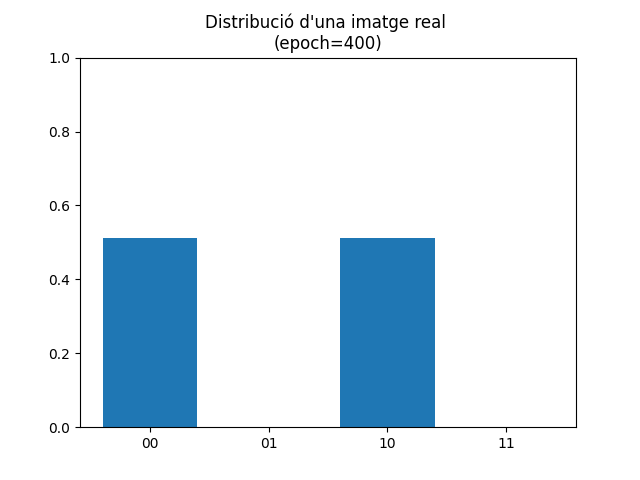
\includegraphics[width=\linewidth]{figures/model/real_distribution.png}
		\caption{Distribució d'una imatge real} \label{fig:1a}
	\end{subfigure}%
	\hspace*{\fill}   % maximize separation between the subfigures
	\begin{subfigure}{0.51\textwidth}
		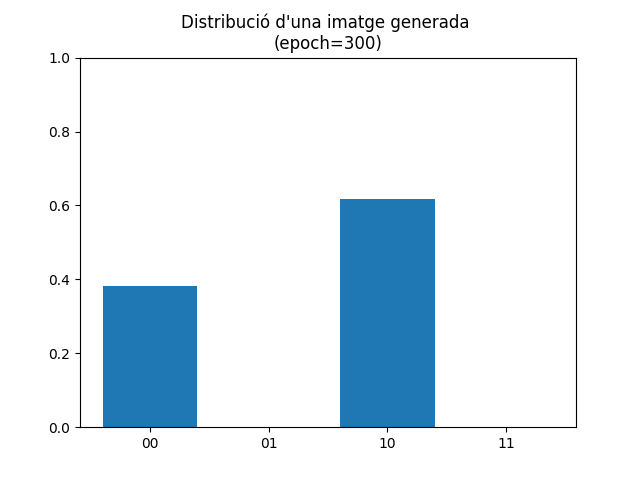
\includegraphics[width=\linewidth]{figures/model/fake_distribution.png}
		\caption{Distribució d'una imatge generada} \label{fig:1b}
	\end{subfigure}%
	\hspace*{\fill}
	\caption{Comparació d'una imatge generada i una real, quan el model ha assolit la convergència. En el eix Y es pot veure el valor d'un píxel, mentre que en l'eix X estan els píxels. }   % maximizeseparation between the subfigures
\end{figure}
\begin{figure}
	\label{fig:labels_loss_400}
	\begin{subfigure}{0.45\textwidth}
		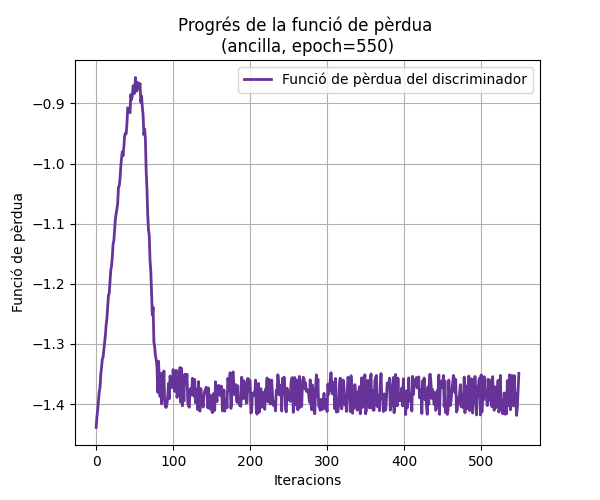
\includegraphics[width=\linewidth]{figures/model/loss_plot.png}
		\caption{Funció de pèrdua per cada iteració. A partir de l'iteració 175, es pot veure com el valor de la funció s'estabilitza en l'interval $(-1.35, -1.4)$, això concorda amb els valors de les etiquetes en les mateixes iteracions, ja que $\log(\frac{1}{2}) + \log(1-\frac{1}{2}) \simeq -1.38$.}\label{fig:loss_400}
	\end{subfigure}%
	\hspace*{\fill}   % maximize separation between the subfigures
	\begin{subfigure}{0.45\textwidth}
		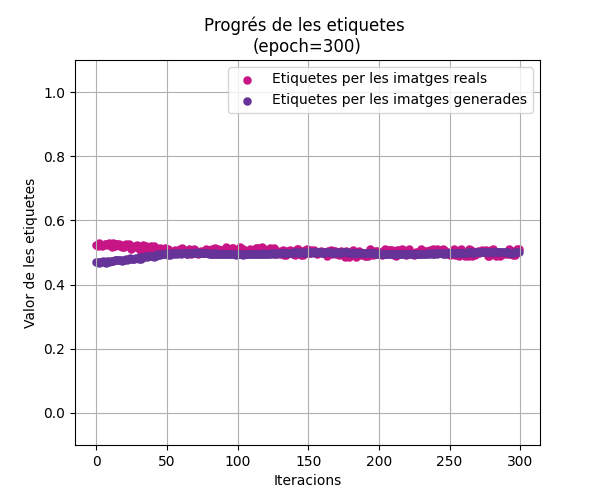
\includegraphics[width=\linewidth]{figures/model/labels_plot.png}
		\caption{Etiquetes per les imatges reals i generades per cada iteració. Es pot observar que els valors de les etiquetes per les imatges reals són més inestables que els valors de les generades. Això es perquè les imatges reals tenen una major variació en els valors dels píxels, mentre que en les generades aquest fet no es tan notable. Per tant el discriminador assigna etiquetes amb una major variació.} \label{fig:labels_400}
	\end{subfigure}%
	\hspace*{\fill}
	\caption{En pot veure com per l'iteració 250, el model ja s'ha estabilitzat, ja que les etiquetes i el valor de la funció de pèrdua convergeixen en un valor.}% maximizeseparation between the subfigures
\end{figure}

En la figura, \ref{fig:labels_400}, es pot veure com les etiquetes pels dos tipus d'imatges van oscil·lant fins a estabilitzar-se. El mateix es pot dir per la funció de pèrdua \ref{fig:loss_400}.  

Degut a que aquests gràfics són molt semblants als seus anàlegs de les GANs clàssiques i que les distribucions reals i generades són pràcticament iguals, com es pot veure a la figura \ref{fig:comp_imatge}. Considero que el model funciona correctament. 



Abans he especificat que al cap de $400$ iteracions podem tenir la garantir d'arribar al punt d'equilibri, no obstant, es pot arribar a aquest punt amb menys iteracions, el que vull dir es que amb $400$ de segur que s'arriva. Això és perquè, com a tots els model de \textit{machine learning} hi ha una part de sort implicada, si els paràmetres inicials són més semblants als paràmetres desitjats, el model assoli-ra la convergència més ràpidament. Per més detalls l'execució del model es pot veure l'apèndix XXX. Tanmateix, per més informació sobre la part experimental del treball es pot veure en l'apèndix XXX.1, en aquest capítol he omitit coses interessants com el meu intent de generació d'imatges a color. 
 
\chapter{Realització del experiment} 

Una vegada havia confirmat el correcte funcionament del model, vaig alterar el generador per poder acomodar els dos tipus de circuits quàntics que necessitava, uns amb un sistema ancilla, i uns altres sense.

Un sistema ancilla, són un grup de qubits sobre els quals es donen a terme operacions però que no es mesuren per treure el output del circuit. Aquests qubits es pot veure molt clar en la figura, \todo{poner figura}. 

Primer de tot he de mencionar que havia de fer alguns canvis al generador per acomodar aquests qubits ancilla. 

Segon, cal notar que no he seguit exactament els mateixos passos que en l'article original. En ell tenen aquesta equació \cite{QGAN_exp}: 
\begin{equation*}
\rho = \frac{\tr_A(\Pi_A \ket{\psi}\bra{\psi})}{\tr(\Pi_A\otimes I_{2^N-2^{N_A}}\ket{\psi}\bra{\psi})}
\end{equation*}

Com ja he comentat en la secció \ref{par_measurament}, no veig com aquesta equació pot tenir sentit, per tant la vaig ometre del meu experiment. 

L'alternativa que he fet servir són els mesuraments de Qiskit, al definir el circuit especifico quins són els qubits que vull mesurar, que són els qubits que formen part del sistema ancilla. No obstant, no sé exactament que és lo que fa Qiskit amb el mesurament. Però si empro aquest procediment en altres circuits, quals sé com han de funcionar, aquest mètode fa el que m'espero\footnote{Parlo del parells de Bell, els circuits quàntics amb entrellaçament més simples que es poden fer.}. 

L'arxiu que utilitzo per fer els experiments és \code{experiment.py}. En ell es pot veure com defineixo dos discriminadors\footnote{Que són iguals en característiques} i dos generadors, que es diferencien per els circuits que utilitzen, un amb qubits ancilla i l'altre sense. Aquests model s'agrupen en parelles per definir dos qGANs. 

Cal notar que els generadors i els discriminadors\footnote{Al principi pensava no tenir els mateixos paràmetres inicials pels discriminadors, però al veure les gràfiques de les etiquetes, l'efecte que tenen aquests és molt notable. Es pot veure com a vegades les etiquetes comencen en uns valors de $1$ i en altres de $0$. \href{https://drive.google.com/file/d/1kYZ1vmNYU17sofNluXFYnoATLfY5B0jG/view?usp=sharing}{link per veure una imatge amb totes les gràfiques} (perdó per l'informalitat)} comencen amb els mateixos paràmetres, per tant en exactament les mateixes condicions, menys els circuits quàntics es clar. També s'utilitza el mateix dataset i altres hiperparàmetres. 

\section{Anàlisi dels resultats}


 

	
	\chapter{Conclusions}
	\label{chap:conclusions}
	
Una vegada havia implementat la distancia de Férchet per poder avaluar el rendiment dels models, havia arribat a una clara conclusió:

Els models que tenen implementada la funció no-lienal són més eficients. 

No és exactament així perquè s'ha de tenir en compte el temps que triguen en optimitzar-se, no obstant, trec aquesta conclusió pel fet que els models sense la funció no arriben a estabilitzar-se. Fins el que puc veure, es queden oscil·lant entre 'aquestes imatges són idèntiques' i 'encara queda per optimitzar'. En una iteració les imatges són pràcticament iguals i al cap de 20 iteracions es pot diferenciar clarament entre una imatge falsa i una generada. 

Aquest problema no es causat pel discriminador, és el generador el que es queda oscil·lant. No sé molt bé la causa d'aquesta oscil·lació, però està clar que la funció no-lineal té un impacte. Tot i que hi han excepcions, a vegades els models sense la funció no experimenten aquesta oscil·lació. Però cal remarcar que les vegades que passa són notablement més altes que les que no passa. Com es pot veure amb les dades de la taula \ref{tab:oscilations} 

\begin{table}[]
	\resizebox{\textwidth}{!}{%
		\begin{tabular}{c|c|c}
			\hline
			& Presenta oscil·lació & No Presenta oscil·lació \\
			\hline
			Amb Funció No-Lineal & 0 & 6 \\
			\hline
			Sense Funció No-Lineal& 5 & 1 \\
			\hline
		\end{tabular}
	}
	\caption{Les dades provenen d'un total de 6 model, 3 d'ells amb un total de $700$ epoch i els altres 5 amb un total de $550$. El nombre d'iteraccions no hauria d'afectar de cada manera les dades. Degut si hi ha una oscil·lació, es pot veure clarament a partir de les $400$ iteracions. Amb les dades es pot veure que és més probable que un model sense la funció lienal presenti una oscil·lació. Cal notar que cap model amb la funció ha tingut una oscil·lació. Les gràfiques que corresponen a cada model es poden veure en la figura \_.}
	\label{tab:oscilations}
\end{table}

\begin{figure}
	\begin{subfigure}[b]{.32\linewidth}
		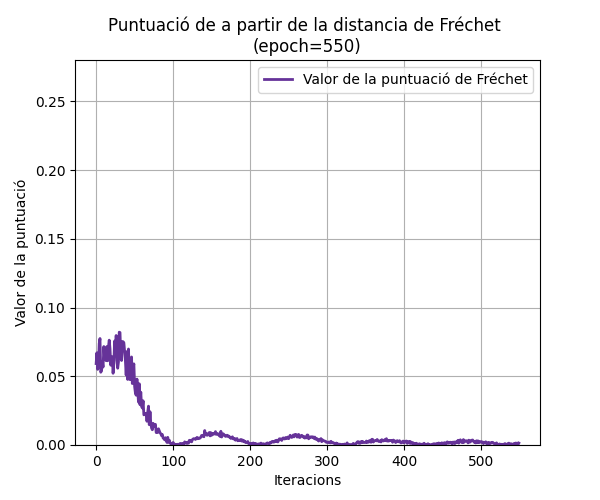
\includegraphics[width=\linewidth]{figures/data/FD_score_1.png}
		\caption{}
	\end{subfigure}
	\begin{subfigure}[b]{.32\linewidth}
		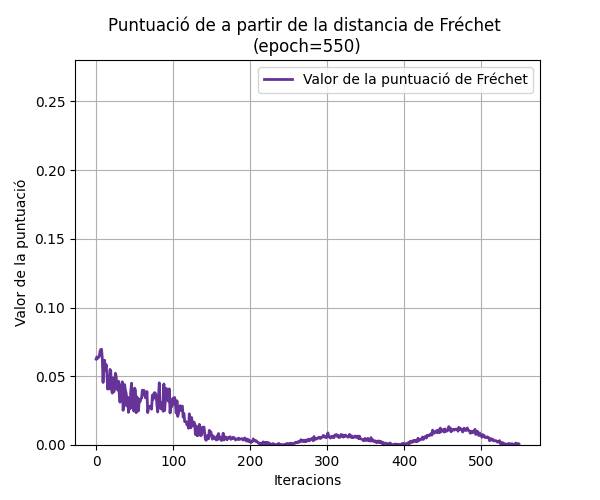
\includegraphics[width=\linewidth]{figures/data/FD_score_2.png}
		\caption{}
	\end{subfigure}
	\begin{subfigure}[b]{.32\linewidth}
		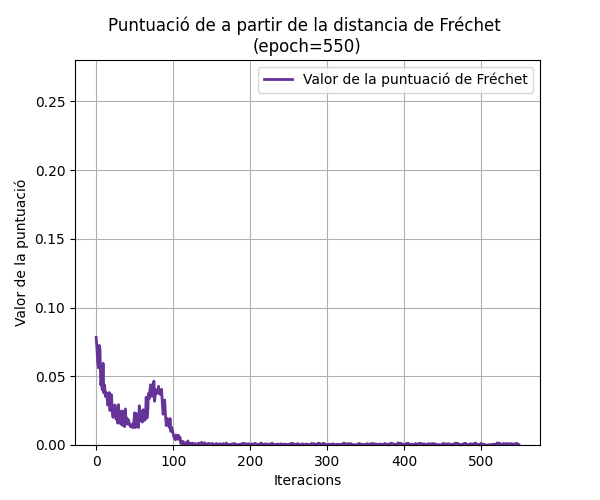
\includegraphics[width=\linewidth]{figures/data/FD_score_3.png}
		\caption{}
	\end{subfigure}
	
	\begin{subfigure}[b]{.32\linewidth}
		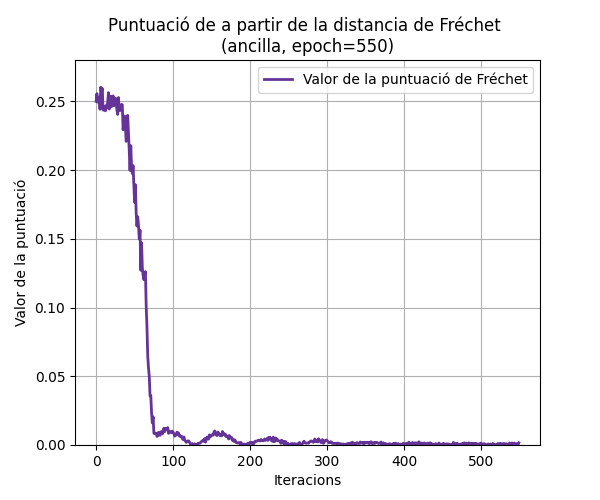
\includegraphics[width=\linewidth]{figures/data/FD_score_A1.png}
		\caption{}
	\end{subfigure}
	\begin{subfigure}[b]{.32\linewidth}
		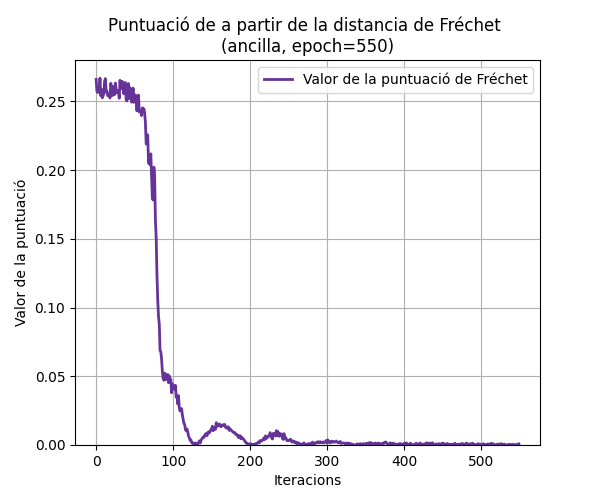
\includegraphics[width=\linewidth]{figures/data/FD_score_A2.png}
		\caption{}
	\end{subfigure}
	\begin{subfigure}[b]{.32\linewidth}
		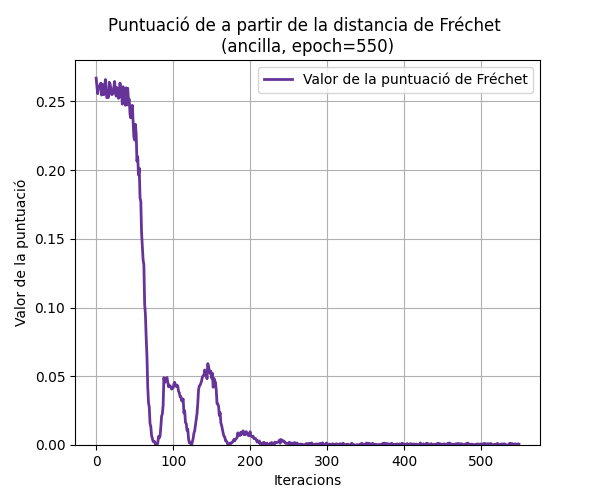
\includegraphics[width=\linewidth]{figures/data/FD_score_A3.png}
		\caption{}
	\end{subfigure}
\label{fig:550_SD_score}
\caption{Totes les gràfiques corresponen a models que s'ha executat al llarg de $550$ iteracions. \textbf{A}, \textbf{B} i \textbf{C}, corresponen a models sense la funció lineal. Es l'únic d'ells que no presenta una oscil·lació és el \textbf{C}. Les gràfiques sense la funció es poden comparar a les d'abaix, les quals representen models amb la funció. Els models han estat creats per parelles, les quals estan organitzades verticalment. Es a dir, les gràfiques \textbf{A} i \textbf{D} representen models que tenen els mateixos paràmetre inicial, que són equivalents. El mateix passa amb \textbf{B} i \textbf{E} i d'una altra banda amb \textbf{C} i \textbf{F}.}
	
\end{figure}

\begin{figure}
	\begin{subfigure}[b]{.32\linewidth}
		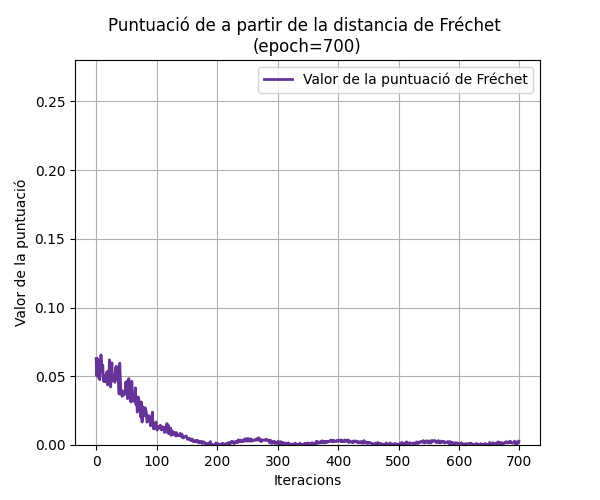
\includegraphics[width=\linewidth]{figures/data/FD_score_4.png}
		\caption{}
	\end{subfigure}
	\begin{subfigure}[b]{.32\linewidth}
		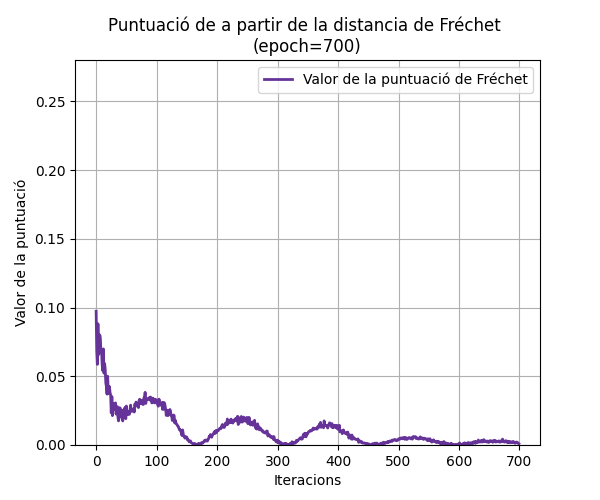
\includegraphics[width=\linewidth]{figures/data/FD_score_5.png}
		\caption{}
	\end{subfigure}
	\begin{subfigure}[b]{.32\linewidth}
		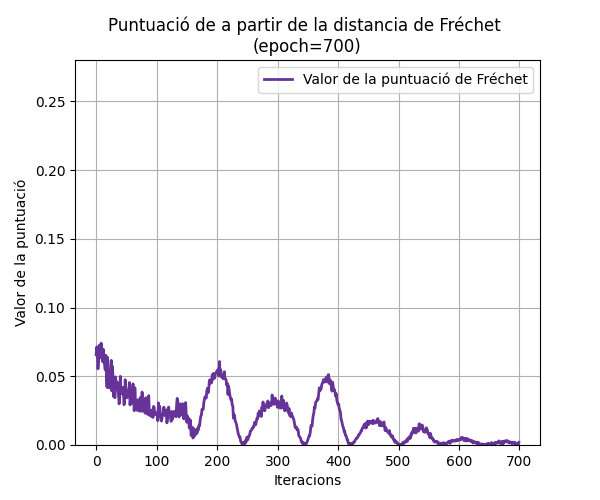
\includegraphics[width=\linewidth]{figures/data/FD_score_6.png}
		\caption{}
	\end{subfigure}
	
	\begin{subfigure}[b]{.32\linewidth}
		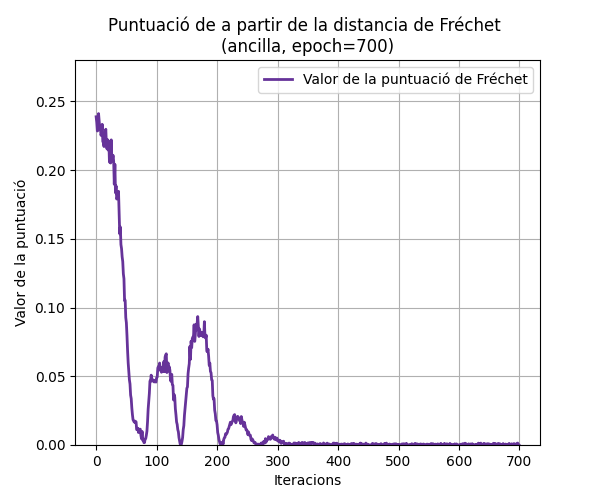
\includegraphics[width=\linewidth]{figures/data/FD_score_A4.png}
		\caption{}
	\end{subfigure}
	\begin{subfigure}[b]{.32\linewidth}
		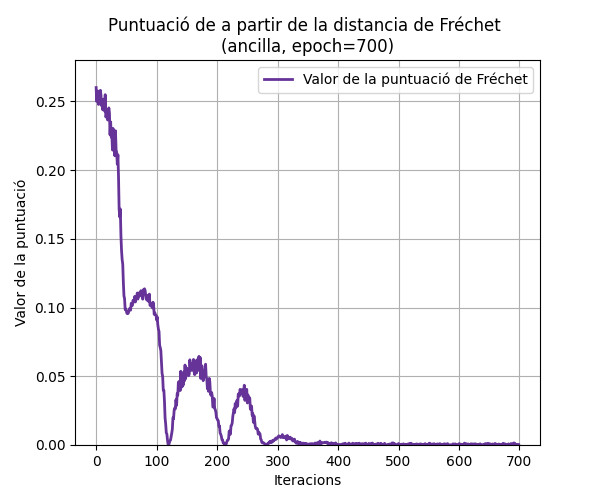
\includegraphics[width=\linewidth]{figures/data/FD_score_A5.png}
		\caption{}
	\end{subfigure}
	\begin{subfigure}[b]{.32\linewidth}
		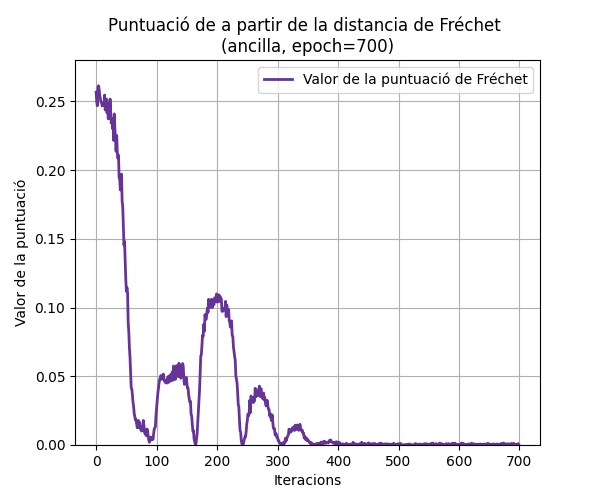
\includegraphics[width=\linewidth]{figures/data/FD_score_A6.png}
		\caption{}
	\end{subfigure}
	\label{fig:700_SD_score}
	\caption{Aquestes gràfiques corresponen a models que s'han executat al llarg de $700$ iteracions. Estan organitzades igual que les gràfiques de la figura \ref{fig:550_SD_score}. En aquests casos, com es pot observar tots els models sense la funció no-lineal presenten les oscil·lacions. No obstant en la gràfica \textbf{A}, aquesta es molt feble. Per veure com afecten les oscil·lacions es pot veure la figura, on estan representades les ultimes imatges que han generat els models que corresponen les gràfiques d'aquesta figura.}
	
\end{figure}

\begin{figure}
	\begin{subfigure}[b]{.32\linewidth}
		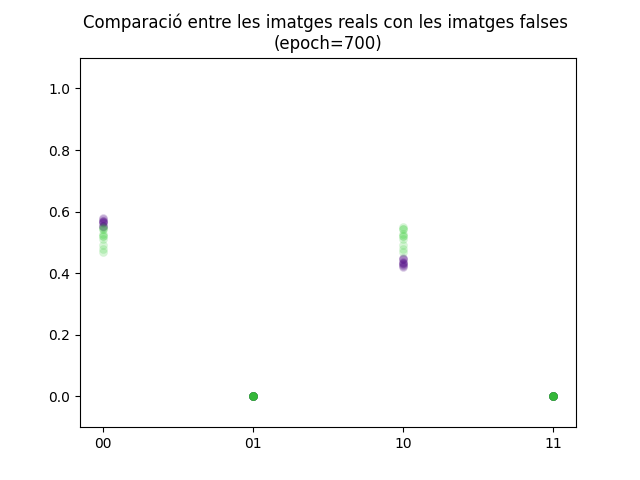
\includegraphics[width=\linewidth]{figures/data/scatter_plot_4.png}
		\caption{}
	\end{subfigure}
	\begin{subfigure}[b]{.32\linewidth}
		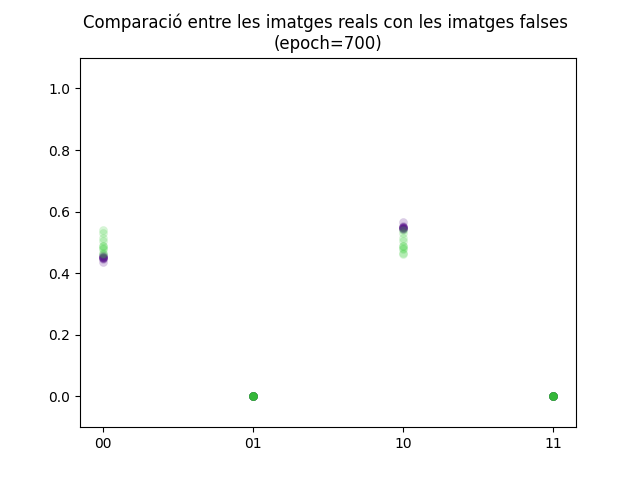
\includegraphics[width=\linewidth]{figures/data/scatter_plot_5.png}
		\caption{}
	\end{subfigure}
	\begin{subfigure}[b]{.32\linewidth}
		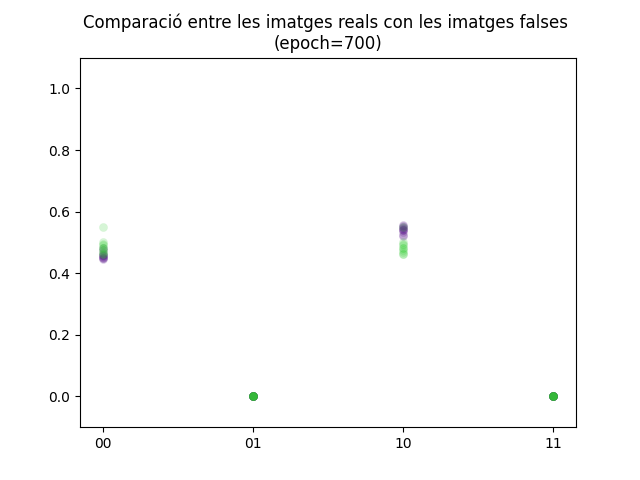
\includegraphics[width=\linewidth]{figures/data/scatter_plot_6.png}
		\caption{}
	\end{subfigure}
	
	\begin{subfigure}[b]{.32\linewidth}
		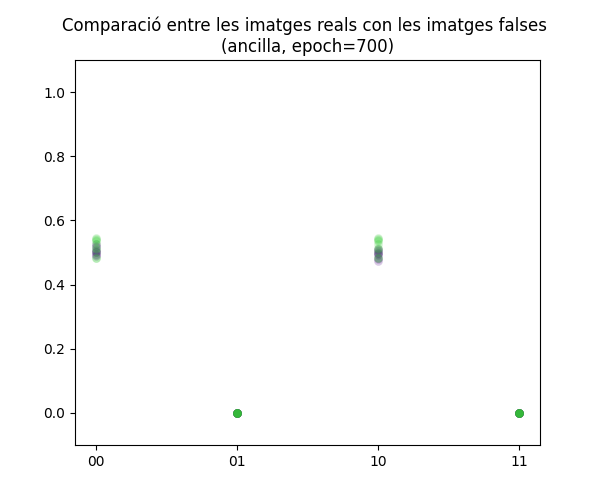
\includegraphics[width=\linewidth]{figures/data/scatter_plot_A4.png}
		\caption{}
	\end{subfigure}
	\begin{subfigure}[b]{.32\linewidth}
		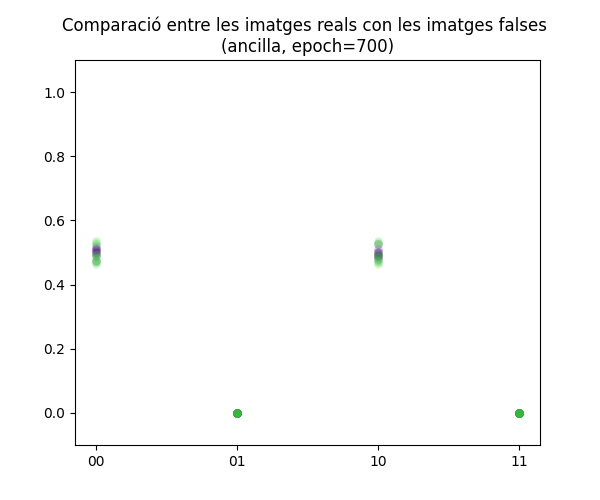
\includegraphics[width=\linewidth]{figures/data/scatter_plot_A5.png}
		\caption{}
	\end{subfigure}
	\begin{subfigure}[b]{.32\linewidth}
		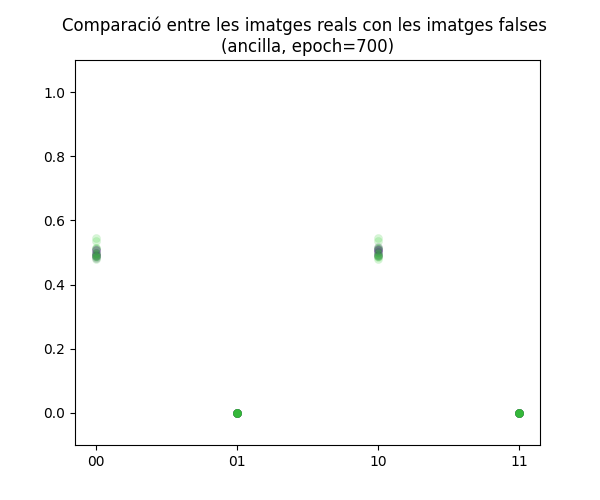
\includegraphics[width=\linewidth]{figures/data/scatter_plot_A6.png}
		\caption{}
	\end{subfigure}
	\label{fig:700_images}
	\caption{Aquestes gràfiques corresponen als mateixos models que els de la figura \ref{fig:700_SD_score}. Les posicions de les gràfiques són les mateixes, per tant si estan en la mateixa posició que les de l'altra figura, corresponen al mateix model. Les imatges generades pels models sense la funció no-lienal  (\textbf{A}, \textbf{C}, \textbf{B}) no s'asemblen a les reals. Es pot veure com els punts de les imatges generades (color violeta) no estan en els mateixos valors. Mentre que en les gràfiques \textbf{D}, \textbf{E} i \textbf{F}, si que ho estan. Els punts violetes sembla que representen la mitjana dels punts verd. També es pot observar que les imatges generades tendeixen a ser més variades que les reals.}
	
\end{figure}





	
	\bibliographystyle{abbrv}
	%\balance
	\bibliography{ref}
	
	\printglossaries
	%\chapter{appendix}
	
	\begin{appendices}
		\chapter{Més àlgebra lineal}
Ja he escrit bastants pàgines sobre àlgebra lineal, però aparentment no eren les suficients perquè estic content amb el treball\footnote{Hi han moltes coses guays i interessants que vull explicar.}, així que aquí hi ha més àlgebra lineal.


\section{Procediment de Gram–Schmidt}\label{gram}
El procediment de Gram-Schmidt és un mètode utilitzat per produir bases per a espais vectorials\cite{QCandQI:GramSchmidt}. Per un espai $V$ amb producte interior de $d$ dimensions amb el set de vectors ${\ket{v_1}, \cdots, \ket{v_d}}$, podem definir una nova base de vectors ortonormals $\{\ket{u}\}$. El primer element d'aquest set és $\ket{u_1} = \ket{v_1}/\norm{\ket{v_1}}$, amb el següent element $\ket{v_{k+1}}$ sent:
$$
\ket{u_{k+1}} = \frac{\ket{v_{k+1}} - \sum_{i=1}^{k} \bra{u_i}\ket{v_{k+1}}\ket{u_i}}{\norm{\ket{v_{k+1}} - \sum_{i=1}^{k} \bra{u_i}\ket{v_{k+1}}\ket{u_i}}}
$$
Per $k$ en el interval $1 \leq k \leq d-1$.

Si seguim per $k$ en $1 \leq k \leq d-1$, obtenim el set de vectors ${\ket{u_1}, \cdots , \ket{u_d}}$ que es una base vàlida per l'espai ortonormal per l'estai $V$. Els vectors creats han de tindre el mateix span\footnote{L'span d'un set de vectors són totes les combinacions lineals possibles amb aquests vectors.} que el dels vectors que originalment eren la base per $V$:
$$
\text{span}(\{\ket{v}\}) = \text{span}(\{\ket{v}\}) = V
$$
Cal notar que l'span de del set base és la definició del espai. En altres paraules, cada vector en $V$ pot ser representat per una combinació del vectors base. 

La prova de que és una base ortonormal és bastant simple:
Podem veure immediatament que els elements  de $\{ \ket{u} \}$ són vectors unitaris perquè estan normalitzats (els vectors $\ket{v_{k+1}} - \sum_{i=1}^{k} \bra{u_i}\ket{v_{k+1}}\ket{u_i}$ estan dividits per la seva norma). També podem veure que són ortogonals els uns als altres mirant que el producte interior entre els doni 0:

Per $k=1$:
$$
\ket{u_2} = \frac{\ket{v_2} - \bra{u_1}\ket{v_2}\ket{u_1}}{\norm{\ket{v_2} - \bra{u_1}\ket{v_2}\ket{u_1}}}
$$
Per tant el producte interior amb $\ket{v_1}$ és:
$$
\begin{aligned}
\bra{u_1}\ket{u_2} 
&= \bra{u_1} \left( \frac{\ket{v_2} - \bra{u_1}\ket{v_2}\ket{u_1}}{\norm{\ket{v_2} - \bra{u_1}\ket{v_2}\ket{u_1}}} \right) \\
&= \frac{\bra{u_1}\ket{v_2} - \bra{u_1}\ket{v_2}\bra{u_1}\ket{u_1}}{\norm{\ket{v_2} - \bra{u_1}\ket{v_2}\ket{u_1}}} \\
&= 0
\end{aligned}
$$
Per inducció podem veure que per $j \leq d$, amb $d$ sent la dimensió del espai vectorial:
$$
\begin{aligned}
	\bra{u_j}\ket{u_{n+1}} 
	& = \bra{u_j} \left( \frac{\ket{v_{n+1}} - \sum_{i=1}^{n} \bra{u_i}\ket{v_{n+1}}\ket{u_i}}{\norm{\ket{v_{n+1}} - \sum_{i=1}^{n} \bra{u_i}\ket{v_{n+1}}\ket{u_i}}} \right) \\
	& = \frac{\bra{u_j}\ket{v_{n+1}} - \sum_{i=1}^{n} \bra{u_i}\ket{v_{n+1}} \bra{u_j}\ket{u_i}}{\norm{\ket{v_{n+1}} - \sum_{i=1}^{n} \bra{u_i}\ket{v_{n+1}} \ket{u_i}}} \\
	& = \frac{\bra{u_j}\ket{v_{n+1}} - \sum_{i=1}^{n} \bra{u_i}\ket{v_{n+1}} \delta_{ij}}{\norm{\ket{v_{n+1}} - \sum_{i=1}^{n} \bra{u_i}\ket{v_{n+1}} \ket{u_i}}} \\
	& = \frac{\bra{u_j}\ket{v_{n+1}} - \bra{u_j}\ket{v_{n+1}}}{\norm{\ket{v_{n+1}} - \sum_{i=1}^{n} \bra{u_i}\ket{v_{n+1}} \ket{u_i}}} \\
	& = 0	\\
\end{aligned}
$$
Tot això no és veu molt clar al principi però cal recordar que el producte interior de dos vectors ortonormals és zero, i que el producte interior entre el mateix vector unitari és un.

\section{Curs ràpid de la notació de Dirac}
A la taula següent hi ha un resum de conceptes matemàtics de l'àlgebra lineal importants expressats en la notació de Dirac\footnote{La notació utilitzada per un espai vectorial complex i l'espai dels nombres complex no són de la notació de Dirac estàndard, però les poso per explicar el que signifiquen.} \cite{QCandQI:dirac_notation}

\begin{tabular}{ p{2cm}|p{12cm} }
	\hline
	Notació & Descripció\\
	\hline
	\hline
	$z$ & Nombre complex    \\
	$z^{*}$ & Conjugat complex d'un nombre complex $z$. $(a+ bi)^{*} = (a -bi)$\\
	$\ket{\psi} $ & Vector amb una etiqueta $\psi$. Conegut com \textit{ket}\\
	$\ket{\psi}^T$ & Transposada d'un vector $\ket{\psi}$ \\
	$\ket{\psi}^\dag $ &  Conjugat Hermitià d'un vector. $\ket{\psi}^\dag = (\ket{\psi}^T)^* $\\
	$\bra{\psi} $ & Vector dual a $\ket{\psi}$. $ \ket{\psi} = \bra{\psi}^{\dag}$ i $\bra{\psi} = \ket{\psi}^\dag$. Conegut com \textit{bra}\\
	$ \bra{\varphi}\ket{\psi} $ & Producte interior dels vectors $\bra{\varphi}$ i $\ket{\psi}$ \\
	$ \ket{\varphi}\bra{\psi} $ & Producte exterior del vectors $\bra{\varphi}$ i $\ket{\psi}$ \\
	$ \ket{\psi}\otimes\ket{\varphi}$ & Producte tensorial del vectors $\ket{\varphi}$ i $\ket{\psi}$ \\
	$ 0 $ & Vector zero i operador zero \\
	$ \mathbb{I}_n $ & Matriu identitat de dimensions $n\times n$ \\
	$ \mathbb{C}_n $ & Espai vectorial complex de dimensió $n$ \\
	$ \mathbb{C}_1$ o $\mathbb{C} $ & Espai del nombres complexos \\
	
\end{tabular}




\chapter{Computació Quàntica vs Mecànica Quàntica}
En la introducció havia mencionat que una de les raons per les quals havia començat a aprendre i recercar sobre computació quàntica era perquè era fàcil, en aquest apèndix explicaré exactament a que em refereixo per això amb un exemple pràctic. Dic que és fàcil, perquè si ho és, si es compara la computació quàntica amb la mecànica quàntica. Presentaré un exemple pràctic per il·lutrar-lo.  

En mecànica quàntica la manera més usual de representar els estats quàntics, com els orbitals d'un àtom d'hidrogen, és a través de \textit{wavefunctions} o funcions d'ona, no es solen representar mitjançant vectors d'estat. Aquestes funcions d'ona són molt útils i poden representar casos més generals que els vectors d'estat. No obstant, treballar amb elles és molt més complicat degut a que són funcions que depenen del temps, no son vectors. Això implica que s'han d'utilitzar altres operacions per normalitzar les funcions, determinar com evolucionen en el temps o per fer mesures. A continuació faré una comparació entre normalitzar una funció d'ona i un vectors d'estat.

\section{Normalitzar}
Degut a l'interpretació probabilística dels vectors d'estat i de les funcions d'ona, aquests objectes han de ser normalitzats perquè la suma de la probabilitats del possibles estats de mesura sigui $1$. 

Per una funció d'ona $\Psi(x,t)$ que representa una partícula, la probabilitat de trobar aquesta partícula en un punt $x$ és $\abs{\Psi(x,t)}^2$. Per tant, la funció d'ona ha de ser normalitza seguint la fórmula: 
\begin{equation}
\int_{-\infty}^{+\infty}\abs{\Psi(x,t)}^2\, dx\ = 1
\label{eq:norm_wave}
\end{equation}

Degut a que la funció d'ona evoluciona a través del temps d'acord amb l'equació de Schrödinger, veure la figura \ref{fig:schro}, qualsevol solució d'aquesta equació ha d'estar també normalitzada. En altres paraules, aquesta equació ha de preservar la normalització de les funcions d'ona \cite{IntroQM:normalizing}.
\begin{figure}[H]
	$$
	i\hslash \pdv{\Psi}{t} = -\frac{\hslash^2}{2m}\pdv[2]{\Psi}{x}+V\Psi
	$$
	\caption{\textbf{Equació de Schrödinger}. On $\hslash$ és $h/2\pi$, i $V$ és una funció potencial d'energia.}
	\label{fig:schro}
\end{figure}

Podem provar que aquesta equació preserva la fórmula \ref{eq:norm_wave}, començant per la igualtat trivial:
$$
\dv{t} \int_{-\infty}^{+\infty}\abs{\Psi(x,t)}^2\, dx\ = \pdv{t} \int_{-\infty}^{+\infty}\abs{\Psi(x,t)}^2\, dx
$$
Per la regla del producte tenim que \footnote{A partir d'ara escriuré  $\Psi(x,t)$ simplement com $\Psi$ per no fer les equacions tan enrevessades.}:
$$
\pdv{t}\abs{\Psi}^2 = \pdv{t}(\Psi\Psi^*) = \Psi^*\pdv{\Psi}{t} + \pdv{\Psi^*}{t}\Psi
$$
Ara l'equació de Schrödinger diu que
$$
\pdv{\Psi}{t} = \frac{i\hslash}{2m}\pdv[2]{\Psi}{x} -  \frac{i}{\hslash}V\Psi
$$
després calculant el complex conjugat tenim que 
$$
\pdv{\Psi^*}{t} = - \frac{i\hslash}{2m}\pdv[2]{\Psi^*}{x} + \frac{i}{\hslash}V\Psi^*
$$
per tant
$$
\pdv{t}\abs{\Psi}^2 = \frac{i\hslash}{2m} \left( \Psi^*\pdv[2]{\Psi}{x} - \pdv[2]{\Psi^*}{x}\Psi \right) = \pdv{x} \left[ \frac{i\hslash}{2m} \left(\Psi^*\pdv{\Psi}{x} - \pdv{\Psi^*}{x}\Psi\right)\right]
$$
finalment podem avaluar l'integral del principi:
$$
\dv{t} \int_{-\infty}^{+\infty}\abs{\Psi(x,t)}^2\, dx\ = \frac{i\hslash}{2m} \left( \Psi^*\pdv{\Psi}{x} - \pdv{\Psi^*}{x}\Psi \right) \Big|_{-\infty}^{+\infty}
$$
Degut a que $\Psi(x,t)$ ha de convergir a zero quan $x$ va cap a infinit, es veritat que:
$$
\dv{t} \int_{-\infty}^{+\infty}\abs{\Psi(x,t)}^2\, dx\ = 0
$$
Es pot veure que l'integral es constant i per tant quan $\Psi$ es normalitzada a $t=0$, es queda d'aquesta manera per qualsevol $t$ (positiu es clar). 

\chapter{Polarització d'un fotó}
\label{appendix:optics}
En l'equació \ref{eq:photon_state} he excluit el concepte de fase, que determina el tipus de polarització que té un fotó. Hi han 3 tipus:
\begin{enumerate}
	\item \textbf{Linear:}
	Un fotó té polarització lineal quan els angles de la fase $\alpha_x$, $\alpha_y$ en els estats base $\ket{x},\ket{y}$ són iguals:
	\begin{align*}
		\ket{\nearrow} &= \cos(\theta) e^{i\alpha_x}\ket{x} + \cos(\theta)e^{i\alpha_y}\ket{y} \\
		&= [\cos(\theta)\ket{x} + \sin(\theta)\ket{y}]e^{i\alpha}
	\end{align*}
	On $\alpha=\alpha_x=\alpha_y$.
	\item \textbf{Circular:}
	Quan els angles $\alpha_x$, $\alpha_y$ son separats per exactament $\frac{\pi}{2}$ i la amplitud per les dos bases és la mateixa:
	\begin{align*}
		\ket{\nearrow} &= \frac{1}{\sqrt{2}}\cos(\theta)e^{i\alpha_x}\ket{x} \pm i\frac{1}{\sqrt{2}}\sin(\theta)e^{i\alpha_y}\ket{y} \\
					   &= [\cos(\theta)e^{i\alpha_x}\ket{x} \pm i\sin(\theta)e^{i\alpha_y}\ket{y}]\frac{1}{\sqrt{2}}
	\end{align*}
	On el signe $\pm$ indica la diferencia entre la diferencia entre la polarització circular cap a la dreta o la esquerra, amb $+$ i $-$, respectivament.
	\item \textbf{El·líptica:}
	On els angles $\alpha_x$, $\alpha_y$ son diferents per una quantitat arbitraria\footnote{Però que no sigui la quantitat que dona a terme la polarització circular.}:
	$$
	\ket{\nearrow} = \cos(\theta)e^{i\alpha_x}\ket{x} + \sin(\theta)e^{i\alpha_y}\ket{y}
	$$
	Aquest és el cas més general.
	
\end{enumerate}

\chapter{Complexitat i algoritmes quàntics}
\label{complexity}
En ciència de la computació existeix el concepte de \textit{Big-O Notation}, una forma d'expressar lo eficients que són els algoritmes per fer certes tasques, en altres paraules la complexitat dels algoritmes. Bàsicament es una forma de classificar-los segon la rapidesa que tenen en ver la tasca que els correspon, aquesta rapidesa no és mesura en segons, degut a que aquesta mètrica pot variar d'ordinador a ordinador per les diferencies en hardware que aquest poden tindre. En canvi es mesure en nombre d'operacions o temps directament, però sense unitats. 

La \textit{Big-O Notation} consisteixes en definir el temps màxim que necessita un algoritme, es denota com $O(\cdot)$ on l'argument usualment depèn de $n$ que és la mida del input al algoritme, per exemple un algoritme de cerca ha de cercar a través de $n$ coses. Com a un exemple més concret tenim que un l'algoritme de cerca de cadenes binaries corre en un temps $O(\log_{2} n)$, on $n$ és el nombre de cadenes entre les quals ha de cercar. Recorda que la notació $O(\cdot)$ és el màxim, es a dir es \textit{upper bounded}, això significa que $\log_{2} n$ és la quantitat de temps més gran en la que es troba la cadena, també es possible que es trobi-s'hi a la primera comprovació que es va\footnote{Que la primera cadena que es cerca, és la que s'ha de trobar.}, llavors l'algoritme acabaria en un temps $O(1)$. Simplement és una manera de mirar lo eficients que són els algoritmes en relació a la mida del input que tenen.

Amb aquesta notació tenim una manera de comparar la eficiència que tenen els algoritmes quàntics amb la del clàssics que tenen la mateixa funció. Per il·lustrar aquesta avantatge en eficiència que presenten els algoritmes quàntics, presentaré a continuació els dos algoritmes quàntics més famosos, el de Grover, i el de Shor. Que serveixen per la cerca d'un element en una llista desordenada, i per la factorització en nombres prims respectivament. 

\section{Algoritme de Grover}
Al 1996, Lov Grover va presentar un algoritme quàntic per cercar en dades desordenades \cite{Grover_96} (e.g. cercar el número de telèfon d'una persona en una llista desordenada). Per aquest problema un algoritme clàssic té una complexitat de $O(N)$ cerques\footnote{Una cerca és quan es verifica si un element de la llista és l'element que es cerca.}, mentre que l'algoritme de Grover té una complexitat de $O(\sqrt{N})$, sent substancialment més eficient. En les paraules de Grover \cite{Grover_96} (adaptades), un ordinador clàssic per tindre un probabilitat de $\frac{1}{2}$ de trobar el número de telèfon d'una persona en una llista desordenada necessita mirar a un mínim de $\frac{N}{2}$ números, mentre que amb el seu s'obté el número de telèfon en només $O(\sqrt{N})$ passos\footnote{Per passos entenc que es refereix al nombre de vegades que es mira al oracle, es a dir, el nombre que de vegades que es verifica si s'ha trobar l'element que es cerca.}.

L'algoritme funciona de la següent manera:
Agafar un sistema de $n$ qubits en l'estat $\ket{0}$ que resulten en una combinació de $N = 2^n$ estats. Aplicar una distribució uniforme als qubits, es a dir, aplicar portes Hadamard a tots els qubits, tenint al final un estat resultant $\ket{s}$:
\begin{equation*}
	\ket{s} = \frac{1}{\sqrt{N}} \sum_{x=0}^{2^n-1} \ket{x}
\end{equation*}
Repetir $\approx \frac{\pi}{4}\sqrt{N}$ vegades, el operador de Grover $G$, que consisteix en el següent conjunt d'instruccions:
\begin{algorithmic}[1]
	\State{Aplicar el \textit{Oracle} $U_{\omega}$}
	\State{Aplicar portes Hadamard a tots els qubits}
	\State{Aplicar el \textit{Grover diffusion operator} $U_{s} = 2\ket{s}\bra{s} - I$}
	\State{Aplicar una altre vegada les portes Hadamard}
\end{algorithmic}


El \textit{oracle} és un tipus de funció que s'utilitza en els algoritmes de cerca, té la finalitat de reconèixer si un element és l'element que s'està cercant. En els algoritmes de cerca es construeixen al voltant de l'\textit{oracle}, diversos algoritmes tenen diverses formes de consultar al oracle. A més a més, la quantitat de consultes a l'\textit{oracle} serveixen per quantificar la complexitat del algoritme, a més consultes, més ineficient és l'algoritme. 

Al veure el procediment de l'algoritme es pot veure l\textit{oracle} es consulta aproximadament $\frac{\pi}{4}\sqrt{N}$, vegades, d'aquesta manera resultat en una complexitat aproximada de $O(\sqrt{N})$, on $N=2^{n}$ per $n$ qubits, com ja he esmentat anteriorment. 

No entraré més en profunditat sobre aquest algoritme, perquè sinó hauré d'introduir més conceptes de computació quàntica com ara la fase d'un estat, o començar a utilitzar notació més complicada que també hauré d'explicar. Em sap greu, perquè és un algoritme que funciona d'una manera bonica de veure. També em sembla el millor algoritme per poder explicar una de les millors característiques de la computació quàntica, tenir algoritmes que et descarten automàticament els estats dolents dintre d'una combinació d'estats, d'aquesta manera lliurant un estat concret desitjat de entre la combinació. En el cas de l'algoritme de Grover aquest estat desitjat, és l'estat que està cercant l'\textit{oracle}. 

\section{Algoritme de Shor}
No explicaré aquest algoritme en profunditat degut a que és molt complex\footnote{Hauria d'introduir nous conceptes com la fase d'un qubit i com efectuar la transformada de Fourier inversa en un circuit quàntic.}, no surt ni en els llibres de texts als quals tinc accés. Simplement em limitaré a explicar quina és la seva utilitat i el compararé amb les seves alternatives clàssiques.

L'algoritme de Shor per la factorització en nombres prims \cite{Shor_97}, és probablement l'algoritme quàntic més famós i més rellevant que hi ha, degut a la gran diferencia en complexitat que té en comparació als seus algoritmes anàlegs clàssics, i degut al gran impacte que tindria la seva implementació en a gran escala. Aquest últim punt és el més interesant i llamatiu, per tant és el que desenvoluparé en major profunditat. 

Actualment totes les dades encriptades que s'envien a través d'internet són encriptades mitjançant la familia de protocols RSA\footnote{RSA són les sigles dels creadors d'aquests protocols; Ron Rivest, Adi Shamir i Leonard Adleman, que al 1977 van publicar els resultats de la seva investigació.  https://dl.acm.org/doi/10.1145/359340.359342}. Aquests protocols són ligerament complicants, no els explicaré, l'únic fet que hem de tenir en compte és que per desencriptar un missatge s'ha de trobar els factors factors prims s'un nombre $n$, es a dir, dos nombres prims $p$ i $q$ que multiplicats donin $n$. Amb aquests nombres es poden saber les claus públiques i privades per encriptar i desencriptar missatges. $n$ seria la clau pública, un nombre que tothom pot coneixer i amb el qual es poden encriptar missatges. Mentres que a partir de $p$ i $q$ es pot trobar la clau privada que correspon a la clau pública, amb la qual es pot descriptar un missatge encriptar amb $n$, per aquesta raó es mantenen els nombres $p$ i $q$ secrets. Es pot entendre la clau pública com un candau que només s'obre amb la clau privada. Cal menciona que a cada clau privada correspond una clau pública, són parellas úniques.   

En encriptació es busca el que diu \textit{one way operations}, es a dir, una operació que si sigui fàcil de fer, però que la seva inversa requereixi de molts recursos computacionals per donar-la a terme. L'operació $n = pq$ compleix aquest requisit, és fàcil muliplicar els nombres prims $p$ i $q$ i trobar $n$, però és molt díficil trobar els nombres $p$ i $q$ sabent $n$, degut a que s'ha de realitzar una factorització de $n$ en nombres prims. Els millors algoritmes per donar a terme aquesta tasca requereixen de moltísim temps computacional en els ordenadors clàssics. Per aquesta raó el protocol RSA s'utilitza ampliament, és molt segur degut a que per saber la clau privada a partir de $n$, es requereix de molt de temps. Amb $n$ sent un nombre de 2048 bits, amb la tecnologia actual no és possible trobar els nombres prims $p$ i $q$ en un temps raonable. Dic raonable perquè es pot arribar a trobar, però es tardaria milers d'anys inclús amb el ordinadors més potents del planeta.

Ara es quan l'algoritme de Shor juga la seva part, com ja he dit s'utilitza per la facorització de nombres primers, i a diferencia dels seus anàlegs clàssics, és extremandament eficient en comparació. En termes de complexitat, aquest algortime pot factoritzar un nombre de $N$ digit en un temps polinomi de $O(\log N)$.  

\chapter{Codi}
En l'apèndix actual presentaré el codi que he utilitzat al llarg del treball. Està organitzat segons el moment en el qual he referenciat el codi en el text. 

IMPORTANT: Si hi ha text en català dintre del codi (n'hi ha en forma de comentaris), no porta accents perquè els paquet que utilitzo per formateixar el codi d'aquesta manera dintre del document no els accepta. Però si es mira el codi en el \href{https://github.com/tomiock/qGAN}{repositori del treball} es pot veure que si que té accents. No em deixa posar ni accents, ni la ce trencada, ni la ele geminada. L'error diu que no són caràcters que estan en Unicode UTF-8, quan si que estan allà, per fet que és un codi que suposadament està internacionalitzat per tots el llenguatges que s'utilitzen 'moderadament'. 

\section{Part I}
\subsection{Capítol 3}

\paragraph{Regressió lienal}
\label{lst:linear_regression}
Codi per efectuar una regressió lineal a dades que es generen al atzar en el mateix arxiu, l'utilitzo per poder generar una gràfic per il·lustrar un exemple de regressió lienal. Aquest tros de codi l'he tret de GitHub\footnote{Gist realitzat per l'usuari \textit{jimimvp}: \href{https://gist.github.com/jimimvp/05ece11fec25d5c8c009af9ba469d6c2}{link}}.

\begin{lstlisting}[language=Python, caption=Regressió lineal]
	import numpy as np
	from matplotlib import pyplot as plt
	import matplotlib
	
	font = {'family' : 'Helvetica',
		'size'   : 18}
	
	matplotlib.rc('font', **font)
	
	# generate the data
	np.random.seed(222)
	X = np.random.normal(0,1, (200, 1))
	w_target = np.random.normal(0,1, (1,1))
	# data + white noise
	y = X@w_target + np.random.normal(0, 1, (200,1))
	
	# least squares
	w_estimate = np.linalg.inv(X.T@X)@X.T@y
	y_estimate = X@w_estimate
	
	# plot the data
	plt.figure(figsize=(15,10))
	plt.scatter(X.flat, y_estimate.flat, label="Prediccio")
	plt.scatter(X.flat, y.flat, color='red', alpha=0.4, label="Dades")
	plt.tight_layout()
	plt.title("Regressio per diferencia de quadrats")
	plt.legend()
	plt.savefig("least_squares.png")
	plt.show()
\end{lstlisting}

\section{Part II}
\subsection{Capítol 6}

\paragraph{Codi original per la xarxa neuronal clàssica}
\label{lst:disc_original}
Està extret del \href{https://github.com/mnielsen/neural-networks-and-deep-learning}{repositori de GitHub de Micheal Nielsen}, concretament del arxiu \code{network.py}.


\begin{lstlisting}[language=Python, caption=Codi original per la xarxa neuronal clàssica]
"""
network.py
~~~~~~~~~~
A module to implement the stochastic gradient descent learning
algorithm for a feedforward neural network.  Gradients are calculated
using backpropagation.  Note that I have focused on making the code
simple, easily readable, and easily modifiable.  It is not optimized,
and omits many desirable features.
"""

#### Libraries
# Standard library
import random

# Third-party libraries
import numpy as np

class Network(object):

	def __init__(self, sizes):
		"""The list ``sizes`` contains the number of neurons in the
		respective layers of the network.  For example, if the list
		was [2, 3, 1] then it would be a three-layer network, with the
		first layer containing 2 neurons, the second layer 3 neurons,
		and the third layer 1 neuron.  The biases and weights for the
		network are initialized randomly, using a Gaussian
		distribution with mean 0, and variance 1.  Note that the first
		layer is assumed to be an input layer, and by convention we
		won't set any biases for those neurons, since biases are only
		ever used in computing the outputs from later layers."""
		self.num_layers = len(sizes)
		self.sizes = sizes
		self.biases = [np.random.randn(y, 1) for y in sizes[1:]]
		self.weights = [np.random.randn(y, x) for x, y in zip(sizes[:-1], sizes[1:])]

	def feedforward(self, a):
		"""Return the output of the network if ``a`` is input."""
		for b, w in zip(self.biases, self.weights):
			a = sigmoid(np.dot(w, a)+b)
		return a

	def SGD(self, training_data, epochs, mini_batch_size, eta, test_data=None):
		"""Train the neural network using mini-batch stochastic
		gradient descent.  The ``training_data`` is a list of tuples
		``(x, y)`` representing the training inputs and the desired
		outputs.  The other non-optional parameters are
		self-explanatory.  If ``test_data`` is provided then the
		network will be evaluated against the test data after each
		epoch, and partial progress printed out.  This is useful for
		tracking progress, but slows things down substantially."""
		if test_data: n_test = len(test_data)
		n = len(training_data)
		for j in xrange(epochs):
			random.shuffle(training_data)
			mini_batches = [training_data[k:k+mini_batch_size] for k in xrange(0, n, mini_batch_size)]
			for mini_batch in mini_batches:
				self.update_mini_batch(mini_batch, eta)
			if test_data:
				print "Epoch {0}: {1} / {2}".format(j, self.evaluate(test_data), n_test)
			else:
				print "Epoch {0} complete".format(j)

	def update_mini_batch(self, mini_batch, eta):
		"""Update the network's weights and biases by applying
		gradient descent using backpropagation to a single mini batch.
		The ``mini_batch`` is a list of tuples ``(x, y)``, and ``eta``
		is the learning rate."""
		nabla_b = [np.zeros(b.shape) for b in self.biases]
		nabla_w = [np.zeros(w.shape) for w in self.weights]
		for x, y in mini_batch:
			delta_nabla_b, delta_nabla_w = self.backprop(x, y)
			nabla_b = [nb+dnb for nb, dnb in zip(nabla_b, delta_nabla_b)]
			nabla_w = [nw+dnw for nw, dnw in zip(nabla_w, delta_nabla_w)]
		self.weights = [w-(eta/len(mini_batch))*nw for w, nw in zip(self.weights, nabla_w)]
		self.biases = [b-(eta/len(mini_batch))*nb for b, nb in zip(self.biases, nabla_b)]

	def backprop(self, x, y):
		"""Return a tuple ``(nabla_b, nabla_w)`` representing the
		gradient for the cost function C_x.  ``nabla_b`` and
		``nabla_w`` are layer-by-layer lists of numpy arrays, similar
		to ``self.biases`` and ``self.weights``."""
		
		nabla_b = [np.zeros(b.shape) for b in self.biases]
		nabla_w = [np.zeros(w.shape) for w in self.weights]
		# feedforward
		activation = x
		activations = [x] # list to store all the activations, layer by layer
		zs = [] # list to store all the z vectors, layer by layer
		for b, w in zip(self.biases, self.weights):
			z = np.dot(w, activation)+b
			zs.append(z)
			activation = sigmoid(z)
			activations.append(activation)
			
		# backward pass
		delta = self.cost_derivative(activations[-1], y) * sigmoid_prime(zs[-1])
		nabla_b[-1] = delta
		nabla_w[-1] = np.dot(delta, activations[-2].transpose())
		# Note that the variable l in the loop below is used a little
		# differently to the notation in Chapter 2 of the book.  Here,
		# l = 1 means the last layer of neurons, l = 2 is the
		# second-last layer, and so on.  It's a renumbering of the
		# scheme in the book, used here to take advantage of the fact
		# that Python can use negative indices in lists.
		for l in xrange(2, self.num_layers):
			z = zs[-l]
			sp = sigmoid_prime(z)
			delta = np.dot(self.weights[-l+1].transpose(), delta) * sp
			nabla_b[-l] = delta
			nabla_w[-l] = np.dot(delta, activations[-l-1].transpose())
		return (nabla_b, nabla_w)

	def evaluate(self, test_data):
		"""Return the number of test inputs for which the neural
		network outputs the correct result. Note that the neural
		network's output is assumed to be the index of whichever
		neuron in the final layer has the highest activation."""
		test_results = [(np.argmax(self.feedforward(x)), y) for (x, y) in test_data]
		return sum(int(x == y) for (x, y) in test_results)

	def cost_derivative(self, output_activations, y):
		"""Return the vector of partial derivatives \partial C_x /
		\partial a for the output activations."""
		return (output_activations-y)

#### Miscellaneous functions
def sigmoid(z):
	"""The sigmoid function."""
	return 1.0/(1.0+np.exp(-z))

def sigmoid_prime(z):
	"""Derivative of the sigmoid function."""
	return sigmoid(z)*(1-sigmoid(z))
\end{lstlisting}

\paragraph{Codi final per el discriminador}
\label{lst:disc_final}
Aquest codi es pot trobar al \href{https://github.com/tomiock/qGAN}{repositori del treball} en l'arxiu \code{discriminator.py}. 

\begin{lstlisting}[language=Python, caption=Codi final pel discriminador]
"""DISCRIMINATOR"""
import json
from typing import Dict, List

import numpy as np

from quantumGAN.functions import BCE_derivative, minimax_derivative_fake, minimax_derivative_real, sigmoid, sigmoid_prime


def load(filename):
	f = open(filename, "r")
	data = json.load(f)
	f.close()
	# cost = getattr(sys.modules[__name__], data["cost"])
	net = ClassicalDiscriminator_that_works(data["sizes"], data["loss"])
	net.weights = [np.array(w) for w in data["weights"]]
	net.biases = [np.array(b) for b in data["biases"]]
	return net


class ClassicalDiscriminator:

	def __init__(	self,
					sizes: List[int],
					type_loss: str) -> None:

		self.num_layers = len(sizes)
		self.sizes = sizes
		self.type_loss = type_loss
		self.data_loss = {"real": [], "fake": []}
		self.ret: Dict[str, any] = {"loss": [],
			"label real": [],
			"label fake": [],
			"label fake time": [],
			"label real time": []}
		self.biases = [np.random.randn(y, ) for y in sizes[1:]]
		self.weights = [np.random.randn(y, x) for x, y in zip(sizes[:-1], sizes[1:])]

	def feedforward(self, a):
		"""Return the output of the network if ``a`` is input."""
		for b, w in zip(self.biases, self.weights):
		a = sigmoid(np.dot(w, a) + b)
		return a

	def predict(self, x):
		# feedforward
		activation = x
		zs = []  # list to store all the z vectors, layer by layer
		for b, w in zip(self.biases, self.weights):
			z = np.dot(w, activation) + b
			zs.append(z)
			activation = sigmoid(z)
		return activation

	def evaluate(self, test_data):
		test_results = [(np.argmax(self.feedforward(x)), y)
		for (x, y) in test_data]
		return sum(int(x == y) for (x, y) in test_results)


	def forwardprop(self, x: np.ndarray):
		activation = x
		activations = [x]  # list to store all the activations, layer by layer
		zs = []  # list to store all the z vectors, layer by layer
		for b, w in zip(self.biases, self.weights):
			z = np.dot(w, activation) + b
			zs.append(z)
			activation = sigmoid(z)
			activations.append(activation)
		return activation, activations, zs

	def backprop_bce(self, image, label):
		"""Return a tuple ``(nabla_b, nabla_w)`` representing the
		gradient for the cost function C_x.  ``nabla_b`` and
		``nabla_w`` are layer-by-layer lists of numpy arrays, similar
		to ``self.biases`` and ``self.weights``."""
		nabla_b = [np.zeros(b.shape) for b in self.biases]
		nabla_w = [np.zeros(w.shape) for w in self.weights]

		# feedforward and back error calculation depending on type of image
		activation, activations, zs = self.forwardprop(image)
		delta = BCE_derivative(activations[-1], label) * sigmoid_prime(zs[-1])

		# backward pass
		nabla_b[-1] = delta
		nabla_w[-1] = np.dot(delta, activations[-2].reshape(1, activations[-2].shape[0]))

		for l in range(2, self.num_layers):
			z = zs[-l]
			delta = np.dot(self.weights[-l + 1].transpose(), delta) * sigmoid_prime(z)
			nabla_b[-l] = delta
			nabla_w[-l] = np.dot(delta.reshape(delta.shape[0], 1), activations[-l - 1].reshape(1, activations[-l - 1].shape[0]))
		return nabla_b, nabla_w, activations[-1]

	def backprop_minimax(self, real_image, fake_image, is_real):
		"""Return a tuple ``(nabla_b, nabla_w)`` representing the
		gradient for the cost function C_x.  ``nabla_b`` and
		``nabla_w`` are layer-by-layer lists of numpy arrays, similar
		to ``self.biases`` and ``self.weights``."""
		nabla_b = [np.zeros(b.shape) for b in self.biases]
		nabla_w = [np.zeros(w.shape) for w in self.weights]

		# feedforward and back error calculation depending on type of image
		activation_real, activations_real, zs_real = self.forwardprop(real_image)
		activation_fake, activations_fake, zs_fake = self.forwardprop(fake_image)

		if is_real:
			delta = minimax_derivative_real(activations_real[-1]) * sigmoid_prime(zs_real[-1])
			activations, zs = activations_real, zs_real
		else:
			delta = minimax_derivative_fake(activations_fake[-1]) * sigmoid_prime(zs_fake[-1])
			activations, zs = activations_fake, zs_fake

		# backward pass
		nabla_b[-1] = delta
		nabla_w[-1] = np.dot(delta, activations[-2].reshape(1, activations[-2].shape[0]))

		for l in range(2, self.num_layers):
			z = zs[-l]
			delta = np.dot(self.weights[-l + 1].transpose(), delta) * sigmoid_prime(z)
			nabla_b[-l] = delta
			nabla_w[-l] = np.dot(delta.reshape(delta.shape[0], 1),
			activations[-l - 1].reshape(1, activations[-l - 1].shape[0]))
		return nabla_b, nabla_w, activations[-1]

	def train_mini_batch(self, mini_batch, learning_rate):
		global label_real, label_fake
		nabla_b = [np.zeros(b.shape) for b in self.biases]
		nabla_w = [np.zeros(w.shape) for w in self.weights]

		if self.type_loss == "binary cross entropy":
			for real_image, fake_image in mini_batch:
				delta_nabla_b, delta_nabla_w, label_real = self.backprop_bce(real_image, np.array([1.]))
				nabla_b = [nb + dnb for nb, dnb in zip(nabla_b, delta_nabla_b)]
				nabla_w = [nw + dnw for nw, dnw in zip(nabla_w, delta_nabla_w)]

				delta_nabla_b, delta_nabla_w, label_fake = self.backprop_bce(fake_image, np.array([0.]))
				nabla_b = [nb + dnb for nb, dnb in zip(nabla_b, delta_nabla_b)]
				nabla_w = [nw + dnw for nw, dnw in zip(nabla_w, delta_nabla_w)]

		elif self.type_loss == "minimax":
			for real_image, fake_image in mini_batch:
				delta_nabla_b, delta_nabla_w, label_real = self.backprop_minimax(real_image, fake_image, True)
				nabla_b = [nb + dnb for nb, dnb in zip(nabla_b, delta_nabla_b)]
				nabla_w = [nw + dnw for nw, dnw in zip(nabla_w, delta_nabla_w)]

				delta_nabla_b, delta_nabla_w, label_fake = self.backprop_minimax(real_image, fake_image, False)
				nabla_b = [nb + dnb for nb, dnb in zip(nabla_b, delta_nabla_b)]
				nabla_w = [nw + dnw for nw, dnw in zip(nabla_w, delta_nabla_w)]
			else:
				raise Exception("type of loss function not valid")

			# gradient descent
			# nabla_w and nabla_b are multiplied by the learning rate
			# and taken the mean of (dividing by the mini batch size)
			self.weights = [w - (learning_rate / len(mini_batch)) * nw
							for w, nw in zip(self.weights, nabla_w)]
			self.biases = [b - (learning_rate / len(mini_batch)) * nb
						   for b, nb in zip(self.biases, nabla_b)]
\end{lstlisting}

\paragraph{Codi per el generador}
\label{lst:gen_final}
Aquest codi es pot trobar al \href{https://github.com/tomiock/qGAN}{repositori del treball} en l'arxiu \code{generador.py}. 

\begin{lstlisting}[language=Python, caption=Codi final pel generador]
"""QUANTUM GENERATOR"""

from typing import Any, Dict, Optional, cast

import numpy as np
import qiskit
from qiskit import ClassicalRegister, QuantumRegister
from qiskit.circuit import QuantumCircuit
from qiskit.circuit.library import TwoLocal
from qiskit.providers.aer import AerSimulator

from quantumGAN.functions import create_entangler_map, create_real_keys, minimax_generator


class QuantumGenerator:

	def __init__(
			self,
			shots: int,
			num_qubits: int,
			num_qubits_ancilla: int,
			generator_circuit: Optional[QuantumCircuit] = None,
			snapshot_dir: Optional[str] = None
	) -> None:

		super().__init__()
		# passar els arguments de la classe a metodes en de classes
		# d'aquesta manera son accessibles per qualsevol funcio dintre de la classe
		self.num_qubits_total = num_qubits
		self.num_qubits_ancilla = num_qubits_ancilla
		self.generator_circuit = generator_circuit
		self.snapshot_dir = snapshot_dir
		self.shots = shots
		self.discriminator = None
		self.ret: Dict[str, Any] = {"loss": []}
		self.simulator = AerSimulator()

	def init_parameters(self):
		"""Inicia els parametres inicial i crea el circuit al qual se li posen els parametres"""
		# iniciacia dels parametres inicials i dels circuits al qual posar aquests parametres
		self.generator_circuit = self.construct_circuit(latent_space_noise=None, to_measure=False)
		# s'ha de crear primer el circuit perque d'aquesta manera es pot saber el nombre de parametres que es necessiten
		self.parameter_values = np.random.normal(np.pi / 2, .1, self.generator_circuit.num_parameters)

	def construct_circuit(self,
						latent_space_noise,
						to_measure: bool):
		"""Crea el circuit quantic des de zero a partir de diversos registres de qubits"""
		if self.num_qubits_ancilla is 0:
			qr = QuantumRegister(self.num_qubits_total, 'q')
			cr = ClassicalRegister(self.num_qubits_total, 'c')
			qc = QuantumCircuit(qr, cr)
		else:
			qr = QuantumRegister(self.num_qubits_total - self.num_qubits_ancilla, 'q')
			anc = QuantumRegister(self.num_qubits_ancilla, 'ancilla')
			cr = ClassicalRegister(self.num_qubits_total - self.num_qubits_ancilla, 'c')
			qc = QuantumCircuit(anc, qr, cr)

		# creacia de la part del circuit que conte la implantacio dels parametres d'input. En cas que no es donin aquests parametres es creen automaticament
		if latent_space_noise is None:
			randoms = np.random.normal(-np.pi * .01, np.pi * .01, self.num_qubits_total)
			init_dist = qiskit.QuantumCircuit(self.num_qubits_total)

			# es col.loca una porta RY en cada qubits i amb un parametre diferent cadascuna
			for index in range(self.num_qubits_total):
				init_dist.ry(randoms[index], index)
		else:
			init_dist = qiskit.QuantumCircuit(self.num_qubits_total)

			for index in range(self.num_qubits_total):
				init_dist.ry(latent_space_noise[index], index)

		# la funcio create_entagler_map crea les parelles de qubits a les qual col.locar les portes CZ
		# en funcio del nombre de qubits
		if self.num_qubits_ancilla is 0:
			entangler_map = create_entangler_map(self.num_qubits_total)
		else:
			entangler_map = create_entangler_map(self.num_qubits_total - self.num_qubits_ancilla)

		# creacio final dels circuits a partir una funcio integrada a Qiskit que va repetint les operacions
		# que se li especifiquen
		ansatz = TwoLocal(int(self.num_qubits_total), 'ry', 'cz', entanglement=entangler_map, reps=1, insert_barriers=True)

		# aqui s'ajunten el circuit que funciona com a input amb el circuit que consisteix en la repeticio
		# de les portes RY i CZ
		qc = qc.compose(init_dist, front=True)
		qc = qc.compose(ansatz, front=False)

		if to_measure:
			qc.measure(qr, cr)

		return qc

	def set_discriminator(self, discriminator) -> None:
		self.discriminator = discriminator

	def get_output(
					self,
					latent_space_noise,
					parameters: Optional[np.ndarray] = None
					):
		"""Retorna un output del generador quan se li dona un estat d'input i opcionalment uns parametres en especific. Els pixels estan compostos per la probabilitat que un qubit resulti en ket_0 en cada base. Per tant, els pixels de l'imatge estan normalitzats amb la norma l-1."""
		real_keys_set, real_keys_list = create_real_keys(self.num_qubits_total - self.num_qubits_ancilla)

		# en cas de que no es donin parametres com a input, es treuen els parametres de la variable
		# self.parameter_values. Es a dir els parametres que es creen automaticament al principi i que es van
		# actualitzant al mateix temps que el model s'optimitza
		if parameters is None:
			parameters = cast(np.ndarray, self.parameter_values)

		qc = self.construct_circuit(latent_space_noise, True)

		parameter_binds = {parameter_id: parameter_value for parameter_id, parameter_value in zip(qc.parameters, parameters)}

		# el metode bind_parametres del circuit quantic
		qc = qc.bind_parameters(parameter_binds)

		# Simulacio dels circuits mitjancant el simulador Aer de Qiskit. El nivell d'optimitzacio es zero, perque al ser circuits petits i que simulen una vegada, no es necessari. Al optimitzar el proces acaba sent mes lent.
		result_ideal = qiskit.execute(experiments=qc,
									  backend=self.simulator,
									  shots=self.shots,
									  optimization_level=0).result()
		counts = result_ideal.get_counts()

		try:
			# creacio de l'imatge resultant
			pixels = np.array([counts[index] for index in list(real_keys_list)])

		except KeyError:
			# aquesta excepcio sorgeix quan en el diccionari dels resultats no estan totes les keys pel fet que qiskit, en cas de que no hi hagi un mesurament en una base, no inclou aquesta base en el diccionari
			keys = counts.keys()
			missing_keys = real_keys_set.difference(keys)
			# s'utilitza un la resta entre dos sets per poder veure quina es la key que falta en el diccionari
			for key_missing in missing_keys:
				counts[key_missing] = 0

			# una vegada es troba les keys que faltaven es crea l'imatge resultant
			pixels = np.array([counts[index] for index in list(real_keys_list)])

		pixels = pixels / self.shots
		return pixels

	def get_output_pixels(
					 	  self,
						  latent_space_noise,
						  params: Optional[np.ndarray] = None
						  ):
		"""Retorna un output del generador quan se li dona un estat d'input i opcionalment uns parametres en especific. Cada pixel es la probabilitat de que un qubits resulti en l'estat ket_0, per tant, els valors cada pixel (que son independents entre si) es troba en l'interval (0, 1) """
		qc = QuantumCircuit(self.num_qubits_total)

		init_dist = qiskit.QuantumCircuit(self.num_qubits_total)
		assert latent_space_noise.shape[0] == self.num_qubits_total

		for num_qubit in range(self.num_qubits_total):
			init_dist.ry(latent_space_noise[num_qubit], num_qubit)

		if params is None:
			params = cast(np.ndarray, self.parameter_values)

		qc.assign_parameters(params)

		# comptes de simular els valors que donara cada qubits, es simula l'estat final del circuit i d'aquest s'extreuen els valors que es mesuraran per a cada qubit
		state_vector = qiskit.quantum_info.Statevector.from_instruction(qc)
		pixels = []
		for qubit in range(self.num_qubits_total):
			# per treure la probabilitat s'utilitza una funcio implementada en Qiskit
			pixels.append(state_vector.probabilities([qubit])[0])

		# creacio de l'imatge resultada a partir de la llista que conte el valor per a cada pixel
		generated_samples = np.array(pixels)
		generated_samples.flatten()

		return generated_samples

	def train_mini_batch(self, mini_batch, learning_rate):
		"""Optimitzacio del generador per una batch d'imatges. Retorna una batch de les imatges generades amb unes imatges reals que poder donar com a input al generador. """
	 	nabla_theta = np.zero_like(self.parameter_values.shape)
		new_images = []

		for _, noise in mini_batch:
			for index, _ in enumerate(self.parameter_values):
				perturbation_vector = np.zeros_like(self.parameter_values)
				perturbation_vector[index] = 1

				# Creacio dels parametres per generar les dues imatges
				pos_params = self.parameter_values + (np.pi / 4) * perturbation_vector
				neg_params = self.parameter_values - (np.pi / 4) * perturbation_vector

				pos_result = self.get_output(noise, parameters=pos_params)  # Generacio imatges
				neg_result = self.get_output(noise, parameters=neg_params)

				pos_result = self.discriminator.predict(pos_result)  # Assignacio de les etiquetes
				neg_result = self.discriminator.predict(neg_result)

				# Diferencia entre les avaluacions de la funcio de perdua entre les dues etiquetes
				gradient = minimax_generator(pos_result) - minimax_generator(neg_result)
				nabla_theta[index] += gradient  # Afegir derivada d'un parametre al gradient
			new_images.append(self.get_output(noise))

		for index, _ in enumerate(self.parameter_values):
			# Actualitzacio dels parametres a traves del gradient
			self.parameter_values[index] += (learning_rate / len(mini_batch)) * nabla_theta[index]

		# Creacio de la batch d'imatges a retornar
		mini_batch = [(datapoint[0], fake_image) for datapoint, fake_image in zip(mini_batch, new_images)]
		return mini_batch
\end{lstlisting}


\paragraph{Definició del model}
\label{lst:qgan}
Aquest codi es pot trobar al \href{https://github.com/tomiock/qGAN}{repositori del treball} en l'arxiu \code{qgan.py}. 
\begin{lstlisting}[language=Python, caption=Codi per la definició del model]
import glob
import os
import json
import random
from datetime import datetime
from typing import List

import imageio
import matplotlib.pyplot as plt
import numpy as np

from quantumGAN.discriminator import ClassicalDiscriminator
from quantumGAN.functions import fechet_distance, minimax, images_to_distribution, images_to_scatter
from quantumGAN.quantum_generator import QuantumGenerator


class Quantum_GAN:

	def __init__(self,
				 generator: QuantumGenerator,
				 discriminator: ClassicalDiscriminator
				 ):

		self.last_batch = None
		now = datetime.now()
		init_time = now.strftime("%d_%m_%Y__%H_%M_%S")
		self.path = "data/run{}".format(init_time)
		self.path_images = self.path + "/images"
		self.filename = "run.txt"

		if not os.path.exists(self.path):
			os.makedirs(self.path)

		if not os.path.exists(self.path_images):
			os.makedirs(self.path_images)

		with open(os.path.join(self.path, self.filename), "w") as file:
			file.write("RUN {} \n".format(init_time))
			file.close()

		self.generator = generator
		self.discriminator = discriminator
		self.loss_series, self.label_real_series, self.label_fake_series, self.FD_score = [], [], [], []

		self.generator.init_parameters()
		self.example_g_circuit = self.generator.construct_circuit(latent_space_noise=None,
									 	 to_measure=False)
		self.generator.set_discriminator(self.discriminator)

	def __repr__(self):
		return "Discriminator Architecture: {} \n Generator Example Circuit: \n{}" \
		.format(self.discriminator.sizes, self.example_g_circuit)

	def store_info(self, epoch, loss, real_label, fake_label):
		file = open(os.path.join(self.path, self.filename), "a")
		file.write("{} epoch LOSS {} Parameters {} REAL {} FAKE {} \n"
		.format(epoch,
				loss,
				self.generator.parameter_values,
				real_label,
				fake_label))
		file.close()

	def plot(self):
		# save data for plotting
		fake_images, real_images = [], []
		for image_batch in self.last_batch:
			fake_images.append(image_batch[1])
			real_images.append(image_batch[0])

		keys, average_result = images_to_distribution(fake_images)
		print(average_result)
		if self.generator.num_qubits_ancilla != 0:
			plt.title(f"Distribucio d'una imatge generada \n(ancilla, epoch={self.num_epochs})")
		else:
			plt.title(f"Distribucio d'una imatge generada \n(epoch={self.num_epochs})")
		plt.ylim(0., 1.)
		plt.bar(keys, average_result)
		plt.savefig(self.path + "/fake_distribution.png")
		plt.clf()

		keys_real, average_result_real = images_to_distribution(real_images)
		print(average_result_real)
		if self.generator.num_qubits_ancilla != 0:
			plt.title(f"Distribucio d'una imatge real \n(ancilla, epoch={self.num_epochs})")
		else:
			plt.title(f"Distribucio d'una imatge real \n(epoch={self.num_epochs})")
		plt.ylim(0., 1.)
		plt.bar(keys_real, average_result_real)
		plt.savefig(self.path + "/real_distribution.png")
		plt.clf()

		y_axis, x_axis = images_to_scatter(fake_images)
		y_axis_real, x_axis_real = images_to_scatter(real_images)
		if self.generator.num_qubits_ancilla != 0:
			plt.title(f"Comparacio entre les imatges reals con les imatges falses \n(ancilla, epoch={self.num_epochs})")
		else:
			plt.title(f"Comparacio entre les imatges reals con les imatges falses \n(epoch={self.num_epochs})")
		plt.ylim(0. - .1, 1. + .1)
		plt.scatter(y_axis, x_axis, label='Valors per les imatges falses',
				 	color='indigo',
					linewidth=.1,
					alpha=.2)
		plt.scatter(y_axis_real, x_axis_real, label='Valors per les imatges reals',
					color='limegreen',
					linewidth=.1,
					alpha=.2)
		plt.savefig(self.path + "/scatter_plot.png")
		plt.clf()

		t_steps = np.arange(self.num_epochs)
		plt.figure(figsize=(6, 5))
		if self.generator.num_qubits_ancilla != 0:
			plt.title(f"Progres de la funcio de perdua \n(ancilla, epoch={self.num_epochs})")
		else:
			plt.title(f"Progres de la funcio de perdua \n(epoch={self.num_epochs})")
		plt.plot(t_steps, self.loss_series, label='Funcio de perdua del discriminador', color='rebeccapurple', linewidth=2)
		plt.grid()
		plt.legend(loc='best')
		plt.xlabel('Iteracions')
		plt.ylabel('Funcio de perdua')
		plt.savefig(self.path + "/loss_plot.png")
		plt.clf()

		t_steps = np.arange(self.num_epochs)
		plt.figure(figsize=(6, 5))
		if self.generator.num_qubits_ancilla != 0:
			plt.title(f"Progres de les etiquetes \n(ancilla, epoch={self.num_epochs})")
		else:
			plt.title(f"Progres de les etiquetes \n(epoch={self.num_epochs})")
		plt.scatter(t_steps, self.label_real_series, label='Etiquetes per les imatges reals',
					color='mediumvioletred',
					linewidth=.1)
		plt.scatter(t_steps, self.label_fake_series, label='Etiquetes per les imatges generades',
					color='rebeccapurple',
					linewidth=.1)
		plt.grid()
		plt.ylim(0. - .1, 1. + .1)
		plt.legend(loc='best')
		plt.xlabel('Iteracions')
		plt.ylabel('Valor de les etiquetes')
		plt.savefig(self.path + "/labels_plot.png")
		plt.clf()

		plt.figure(figsize=(6, 5))
		if self.generator.num_qubits_ancilla != 0:
			plt.title(f"Puntuacio de a partir de la distancia de Frechet \n(ancilla, epoch={self.num_epochs})")
		else:
			plt.title(f"Puntuacio de a partir de la distancia de Frechet \n(epoch={self.num_epochs})")
		plt.plot(t_steps, self.FD_score, label='Valor de la puntuacio de Frechet', color='rebeccapurple', linewidth=2)
		plt.grid()
		plt.legend(loc='best')
		plt.ylim(0., .28)
		plt.xlabel('Iteracions')
		plt.ylabel('Valor de la puntuacio')
		plt.savefig(self.path + "/FD_score.png")
		plt.clf()

	def train(self,
			  num_epochs: int,
			  training_data: List,
		 	  batch_size: int,
			  generator_learning_rate: float,
			  discriminator_learning_rate: float,
			  is_save_images: bool):

		self.num_epochs = num_epochs
		self.training_data = training_data
		self.batch_size = batch_size
		self.batch_size = batch_size
		self.generator_lr = generator_learning_rate
		self.discriminator_lr = discriminator_learning_rate
		self.is_save_images = is_save_images

		noise = self.training_data[0][1]
		time_init = datetime.now()
		for o in range(self.num_epochs):
			mini_batches = create_mini_batches(self.training_data, self.batch_size)
			output_fake = self.generator.get_output(latent_space_noise=mini_batches[0][0][1], parameters=None)

			for mini_batch in mini_batches:
				self.last_batch = self.generator.train_mini_batch(mini_batch, self.generator_lr)
				self.discriminator.train_mini_batch(self.last_batch, self.discriminator_lr)

			output_real = mini_batches[0][0][0]
			if is_save_images:
				self.save_images(self.generator.get_output(latent_space_noise=noise, parameters=None), o)

			self.FD_score.append(fechet_distance(output_real, output_fake))
			label_real, label_fake = self.discriminator.predict(output_real), self.discriminator.predict(output_fake)
			loss_final = 1 / 2 * (minimax(label_real, label_fake) + minimax(label_real, label_fake))

			self.loss_series.append(loss_final)
			self.label_real_series.append(label_real)
			self.label_fake_series.append(label_fake)

			print("Epoch {}: Loss: {}".format(o, loss_final), output_real, output_fake)
			print(label_real[-1], label_fake[-1])
			self.store_info(o, loss_final, label_real, label_fake)

		time_now = datetime.now()
		print((time_now - time_init).total_seconds(), "seconds")

	def save_images(self, image, epoch):
		image_shape = int(image.shape[0] / 2)
		image = image.reshape(image_shape, image_shape)

		plt.imshow(image, cmap='gray', vmax=1., vmin=0.)
		plt.axis('off')
		plt.savefig(self.path_images + '/image_at_epoch_{:04d}.png'.format(epoch))
		plt.clf()

	def create_gif(self):
		anim_file = self.path + '/dcgan.gif'

		with imageio.get_writer(anim_file, mode='I') as writer:
			filenames = glob.glob(self.path_images + '/image*.png')
			filenames = sorted(filenames)

			for filename in filenames:
				image = imageio.imread(filename)
				writer.append_data(image)

			image = imageio.imread(filename)
			writer.append_data(image)

	def save(self):
		"""Save the neural network to the file ``filename``."""
		data = {"batch_size": self.batch_size,
				"D_sizes": self.discriminator.sizes,
				"D_weights": [w.tolist() for w in self.discriminator.weights],
				"D_biases": [b.tolist() for b in self.discriminator.biases],
				"D_loss": self.discriminator.type_loss,
				"Q_parameters": [theta for theta in self.generator.parameter_values],
				"Q_shots": self.generator.shots,
				"Q_num_qubits": self.generator.num_qubits_total,
				"Q_num_qubits_ancilla": self.generator.num_qubits_ancilla,
				"real_labels": self.label_real_series,
				"fake_labels": self.label_fake_series,
				"loss_series": self.loss_series
				}
		f = open(os.path.join(self.path, "data.txt"), "a")
		json.dump(data, f)
		f.close()


	def create_mini_batches(training_data, mini_batch_size):
		n = len(training_data)
		random.shuffle(training_data)
		mini_batches = [
			training_data[k:k + mini_batch_size]
			for k in range(0, n, mini_batch_size)]
		return [mini_batches[0]]


	def load_gan(filename):
		f = open(filename, "r")
		data = json.load(f)
		f.close()
		discriminator = ClassicalDiscriminator(data["D_sizes"], data["D_loss"])

		generator = QuantumGenerator(num_qubits=data["Q_num_qubits"],
									 generator_circuit=None,
									 num_qubits_ancilla=data["Q_num_qubits_ancilla"],
									 shots=data["Q_shots"])

		quantum_gan = Quantum_GAN(generator, discriminator)

		quantum_gan.discriminator.weights = [np.array(w) for w in data["D_weights"]]
		quantum_gan.discriminator.biases = [np.array(b) for b in data["D_biases"]]
		quantum_gan.generator.parameter_values = np.array(data["Q_parameters"])

		1return quantum_gan, data["batch_size"]
	
	
\end{lstlisting}

\paragraph{Execució del model}
\label{lst:main}
Aquest codi es pot trobar al \href{https://github.com/tomiock/qGAN}{repositori del treball} en l'arxiu \code{main.py}. 

\begin{lstlisting}[language=Python, caption=Codi final pel generador]
import numpy as np

from quantumGAN.discriminator import ClassicalDiscriminator
from quantumGAN.qgan import Quantum_GAN
from quantumGAN.quantum_generator import QuantumGenerator

num_qubits: int = 3

# Set number of training epochs
num_epochs = 150
# Batch size
batch_size = 10

train_data = []
for _ in range(800):
	x2 = np.random.uniform(.55, .46, (2,))
	fake_datapoint = np.random.uniform(-np.pi * .01, np.pi * .01, (num_qubits,))
	real_datapoint = np.array([x2[0], 0, x2[0], 0])
	train_data.append((real_datapoint, fake_datapoint))

discriminator = ClassicalDiscriminator(sizes=[4, 16, 8, 1],
									   type_loss="minimax")
generator = QuantumGenerator(num_qubits=num_qubits,
							 generator_circuit=None,
							 num_qubits_ancilla=1,
							 shots=4096)

quantum_gan = Quantum_GAN(generator, discriminator)
print(quantum_gan)
print(num_epochs)
quantum_gan.generator.get_output(fake_datapoint[0], None)
quantum_gan.train(num_epochs, train_data, batch_size, .1, .1, True)

quantum_gan.plot()
quantum_gan.create_gif()
quantum_gan.save()

\end{lstlisting}


\paragraph{Multiprocessament}
Per poder ser més eficient alhora de executar els models, vaig decidir utilitzar una característica molt útil de Python, el \textit{multiprocessing}. Usualment una instancia de Python, es a dir; un arxiu executant-se, només utilitza un nucli del processador a la vegada, però amb \textit{multiprocessing} pots utilitzar múltiples nuclis amb un mateix arxiu, d'aquesta manera executant diverses línies de codi al mateix temps. Per poder executar diversos models a la mateixa vegada i d'una forma simple, vaig utilitzar aquest modul de Python per executar els models dels quals he agafat les dades que he presentat en aquest treball. Aquest codi es pot trobar al \href{https://github.com/tomiock/qGAN}{repositori del treball} en l'arxiu \code{test\_multi.py}. 
\begin{lstlisting}[language=Python, caption=Executar els models amb multiprocessing]
import multiprocessing
import time
import numpy as np

from quantumGAN.discriminator import ClassicalDiscriminator
from quantumGAN.qgan import Quantum_GAN
from quantumGAN.quantum_generator import QuantumGenerator

batch_size = 10

train_data = []
# generacio de les dades
for _ in range(800):
	x2 = np.random.uniform(.55, .46, (2,))
	fake_datapoint = np.random.uniform(-np.pi * .01, np.pi * .01, (4,))
	real_datapoint = np.array([x2[0], 0, x2[0], 0])
	train_data.append((real_datapoint, fake_datapoint))
list_epochs = [550, 550, 550]

example_generator_ancilla = QuantumGenerator(num_qubits=4,
											 generator_circuit=None,
											 num_qubits_ancilla=2,
											 shots=4096)
example_generator = QuantumGenerator(num_qubits=2,
									 generator_circuit=None,
									 num_qubits_ancilla=0,
									 shots=4096)

# generem els parametres inicials d'acord amb el circuit amb un mayor nombre de parametres
circuit_ancilla = example_generator_ancilla.construct_circuit(None, False)
circuit_not_ancilla = example_generator_ancilla.construct_circuit(None, False)

init_parameters_ancilla = np.random.normal(np.pi / 2, .1, circuit_ancilla.num_parameters)

# canviem les dimensions dels parametres perque coincideixin amb les dimensions necessaries pel circuit
# sense qubits ancilla
not_ancilla_list = init_parameters_ancilla.tolist()[
circuit_ancilla.num_parameters - circuit_not_ancilla.num_parameters:]
init_parameters_not_ancilla = np.array(not_ancilla_list)

example_discriminator = discriminator_ancilla = \
ClassicalDiscriminator(sizes=[4, 16, 8, 1], type_loss="minimax")

init_biases_discriminator, init_weights_discriminator = example_discriminator.init_parameters()


def to_train(num_epochs):
	# definicio d'un discriminador pel model amb la funcio no-lineal i una altre pel model que no la te
	discriminator_ancilla = \
		ClassicalDiscriminator(sizes=[4, 16, 8, 1], type_loss="minimax")
	discriminator_not_ancilla = \
		ClassicalDiscriminator(sizes=[4, 16, 8, 1], type_loss="minimax")

	# es defineix un generador que te la funcio no-lienal integrada en el circuit
	generator_ancilla = \
		QuantumGenerator(num_qubits=4,
						 generator_circuit=None,
						 num_qubits_ancilla=2,  # IMPORTANT
						 shots=4096)
	# i un altre generador que no te la funcio no-lineal
	generator_not_ancilla = \
		QuantumGenerator(num_qubits=2,
     					 generator_circuit=None,
						 num_qubits_ancilla=0,  # IMPORTANT
						 shots=4096)

	quantum_gan_ancilla = \
		Quantum_GAN(generator_ancilla, discriminator_ancilla)
	time.sleep(1)
	quantum_gan_not_ancilla = \
		Quantum_GAN(generator_not_ancilla, discriminator_not_ancilla)
	print(quantum_gan_not_ancilla.path)
	print(quantum_gan_ancilla.path)

	# abans de comencar a entrenar el model s'ha de canviar els parametres als definits anteriorment
	quantum_gan_ancilla.generator.parameter_values = init_parameters_ancilla
	quantum_gan_ancilla.discriminator.weights = init_weights_discriminator
	quantum_gan_ancilla.discriminator.biases = init_biases_discriminator
	quantum_gan_ancilla.train(num_epochs, train_data, batch_size, .1, .1, False)

	quantum_gan_not_ancilla.generator.parameter_values = init_parameters_not_ancilla
	quantum_gan_not_ancilla.discriminator.weights = init_weights_discriminator
	quantum_gan_not_ancilla.discriminator.biases = init_biases_discriminator
	quantum_gan_not_ancilla.train(num_epochs, train_data, batch_size, .1, .1, False)

	# una vegada ha acabat l'optimitzacio es creen els grafics per compara l'eficiencia del models
	quantum_gan_not_ancilla.plot()
	quantum_gan_ancilla.plot()


def main():
	# Crear una queue para compartir les dades entre els processos
	# Crear i iniciar el proces de simulacio
	jobs = []
	for epoch in list_epochs:
		simulate = multiprocessing.Process(None, to_train, args=(epoch,))
		jobs.append(simulate)
		time.sleep(2)
		simulate.start()


if __name__ == '__main__':
	main()
\end{lstlisting}


\paragraph{Funcions extres}
Hi han funcions en el codi que utilitzo en diversos arxius, aquestes les defineixo en l'arxiu \code{functions.py}, que es pot trobar al \href{https://github.com/tomiock/qGAN}{repositori del treball}. En aquest arxiu també hi ha una funció que dona a terme una traça parcial a una matriu donada, malgrat que no la he arribat a utilitzar. 
\begin{lstlisting}[language=Python, caption=Funcions varies]
import itertools
import math

import numpy as np
from matplotlib import pyplot as plt


# DATA PROCESSING
from scipy import linalg


def save_images_color(image, epoch):
	plt.imshow(image.reshape(int(image.shape[0] / 3), 1, 3))
	plt.axis('off')
	plt.savefig('images/image_at_epoch_{:04d}.png'.format(epoch))


def create_real_keys(num_qubits):
	lst = [[str(a) for a in i] for i in itertools.product([0, 1], repeat=num_qubits)]
	new_lst = []
	for element in lst:
		word = str()
		for number in element:
			word = word + number
			new_lst.append(word)
	return set(new_lst), new_lst


def create_entangler_map(num_qubits: int):
	lst = [list(i) for i in itertools.combinations(range(num_qubits), 2)]
	index = 0
	entangler_map = []
	for i in reversed(range(num_qubits)):
		try:
			entangler_map.append(lst[index])
			index += i
		except IndexError:
			return entangler_map


def images_to_distribution(batch_image):
	num_images = len(batch_image)
	sum_result = 0
	for image in batch_image:
		sum_result += image
	average_result = sum_result / num_images
	keys = create_real_keys(int(math.sqrt(batch_image[0].shape[0])))[1]
	return keys, average_result


def images_to_scatter(batch_image):
	keys = create_real_keys(int(math.sqrt(batch_image[0].shape[0])))[1]
	x_axis = []
	y_axis = []

	for image in batch_image:
		pixel_count = 0
		for pixel in image:
			x_axis.append(pixel)
			y_axis.append(keys[pixel_count])
			pixel_count += 1

	return y_axis, x_axis

def fechet_distance(image1: np.array, 
					image2: np.array):
	assert image1.shape == image2.shape
	y = np.arange(0, image1.flatten().shape[0])

	matrix_a_cov = np.cov(np.stack((y, image1.flatten()), axis=0))
	matrix_b_cov = np.cov(np.stack((y, image2.flatten()), axis=0))

	to_trace = matrix_a_cov + matrix_b_cov - 2*(linalg.fractional_matrix_power(np.dot(matrix_a_cov, matrix_b_cov), .5))
	return np.abs(image1.mean() - image2.mean())**2 + np.trace(to_trace)


# ACTIVATION FUNCTIONS

def sigmoid(z):
	"""The sigmoid function."""
	return 1.0 / (1.0 + np.exp(-z))


def sigmoid_prime(z):
	"""Derivative of the sigmoid function."""
	return sigmoid(z) * (1 - sigmoid(z))


def relu(z):
	return np.maximum(0, z)


def relu_prime(z):
	z[z <= 0] = 0
	z[z > 0] = 1
	return z


# LOSSES
def MSE_derivative(prediction, y):
	return 2 * (y - prediction)


def MSE(prediction, y):
	return (y - prediction) ** 2


def BCE_derivative(prediction, target):
	# return prediction - target
	return -target / prediction + (1 - target) / (1 - prediction)


def BCE(predictions: np.ndarray, targets: np.ndarray) -> np.ndarray:
	return targets * np.log(predictions) + (1 - targets) * np.log(1 - predictions).mean()


def minimax_derivative_real(real_prediction):
	real_prediction = np.array(real_prediction)
	return np.nan_to_num((-1) * (1 / real_prediction))


def minimax_derivative_fake(fake_prediction):
	fake_prediction = np.array(fake_prediction)
	return np.nan_to_num(1 / (1 - fake_prediction))


def minimax(real_prediction, fake_prediction):
	return np.nan_to_num(np.log(real_prediction) + np.log(1 - fake_prediction))


def minimax_generator(prediction_fake):
	return (-1) * np.log(1 - prediction_fake)


# QUANTUM FUNCTIONS

class Partial_Trace:
	def __init__(self, state: np.array, qubits_out: int, side: str):

		self.state = state
		self.qubits_out = qubits_out
		self.side = side

		if self.state.ndim == 1:
			self.state = np.outer(self.state, self.state)

		self.total_dim = self.state.shape[0]

		self.num_qubits = int(np.log2(self.total_dim))
		self.a_dim = 2 ** (self.num_qubits - self.qubits_out)
		self.b_dim = 2 ** self.qubits_out

		# if self.side == "bot":
		self.basis_b = [_ for _ in np.identity(int(self.b_dim))]
		self.basis_a = [_ for _ in np.identity(int(self.a_dim))]

		# elif self.side == "top":
		#	self.basis_a = [_ for _ in np.identity(int(self.b_dim))]
		#	self.basis_b = [_ for _ in np.identity(int(self.a_dim))]
		#
		# else:
		#	raise NameError("invalid side argument, enter \"bot\" or \"top\"")
		print(self.basis_a, self.basis_b)

	def get_entry(self, index_i, index_j):
		sigma = 0

		if self.side == "bot":
			for k in range(self.qubits_out + 1):
				ab_l = np.kron(self.basis_a[index_i],
						   	   self.basis_b[k])
				ab_r = np.kron(self.basis_a[index_j],
						   	   self.basis_b[k])

				print(ab_r, ab_l)

				right_side = np.dot(self.state, ab_r)
				sigma += np.inner(ab_l, right_side)

		if self.side == "top":
			for k in range(self.qubits_out + 1):
				ba_l = np.kron(self.basis_b[index_i],
							   self.basis_a[k])
				ba_r = np.kron(self.basis_b[index_j],
							   self.basis_a[k])

				print(ba_r, ba_l)

				right_side = np.dot(self.state, ba_r)
				sigma += np.inner(ba_l, right_side)

		return sigma

	def compute_matrix(self):
		a = [_ for _ in range(self.a_dim)]
		b = [__ for __ in range(self.a_dim)]

		entries_pre = [(x, y) for x in a for y in b]
		entries = []

		for i_index, j_index in entries_pre:
			entries.append(self.get_entry(i_index, j_index))

		entries = np.array(entries)
		return entries.reshape(self.a_dim, self.a_dim)

\end{lstlisting}



	\end{appendices}
	
	
\end{document}